\documentclass[11pt]{article}
% Shared packages for SI table/figure masters (input by each master).
\usepackage[margin=0.6in]{geometry}
\usepackage{booktabs}
\usepackage{longtable}
\usepackage{caption}
\usepackage{hyperref}
\usepackage{graphicx}
\usepackage{float}
\usepackage{amsmath}
\usepackage{enumitem}
\graphicspath{{../../figures/}{../}{./}}
\setlength{\parindent}{0pt}
\pagestyle{plain}

\begin{document}

\begin{figure}[H]
\centering
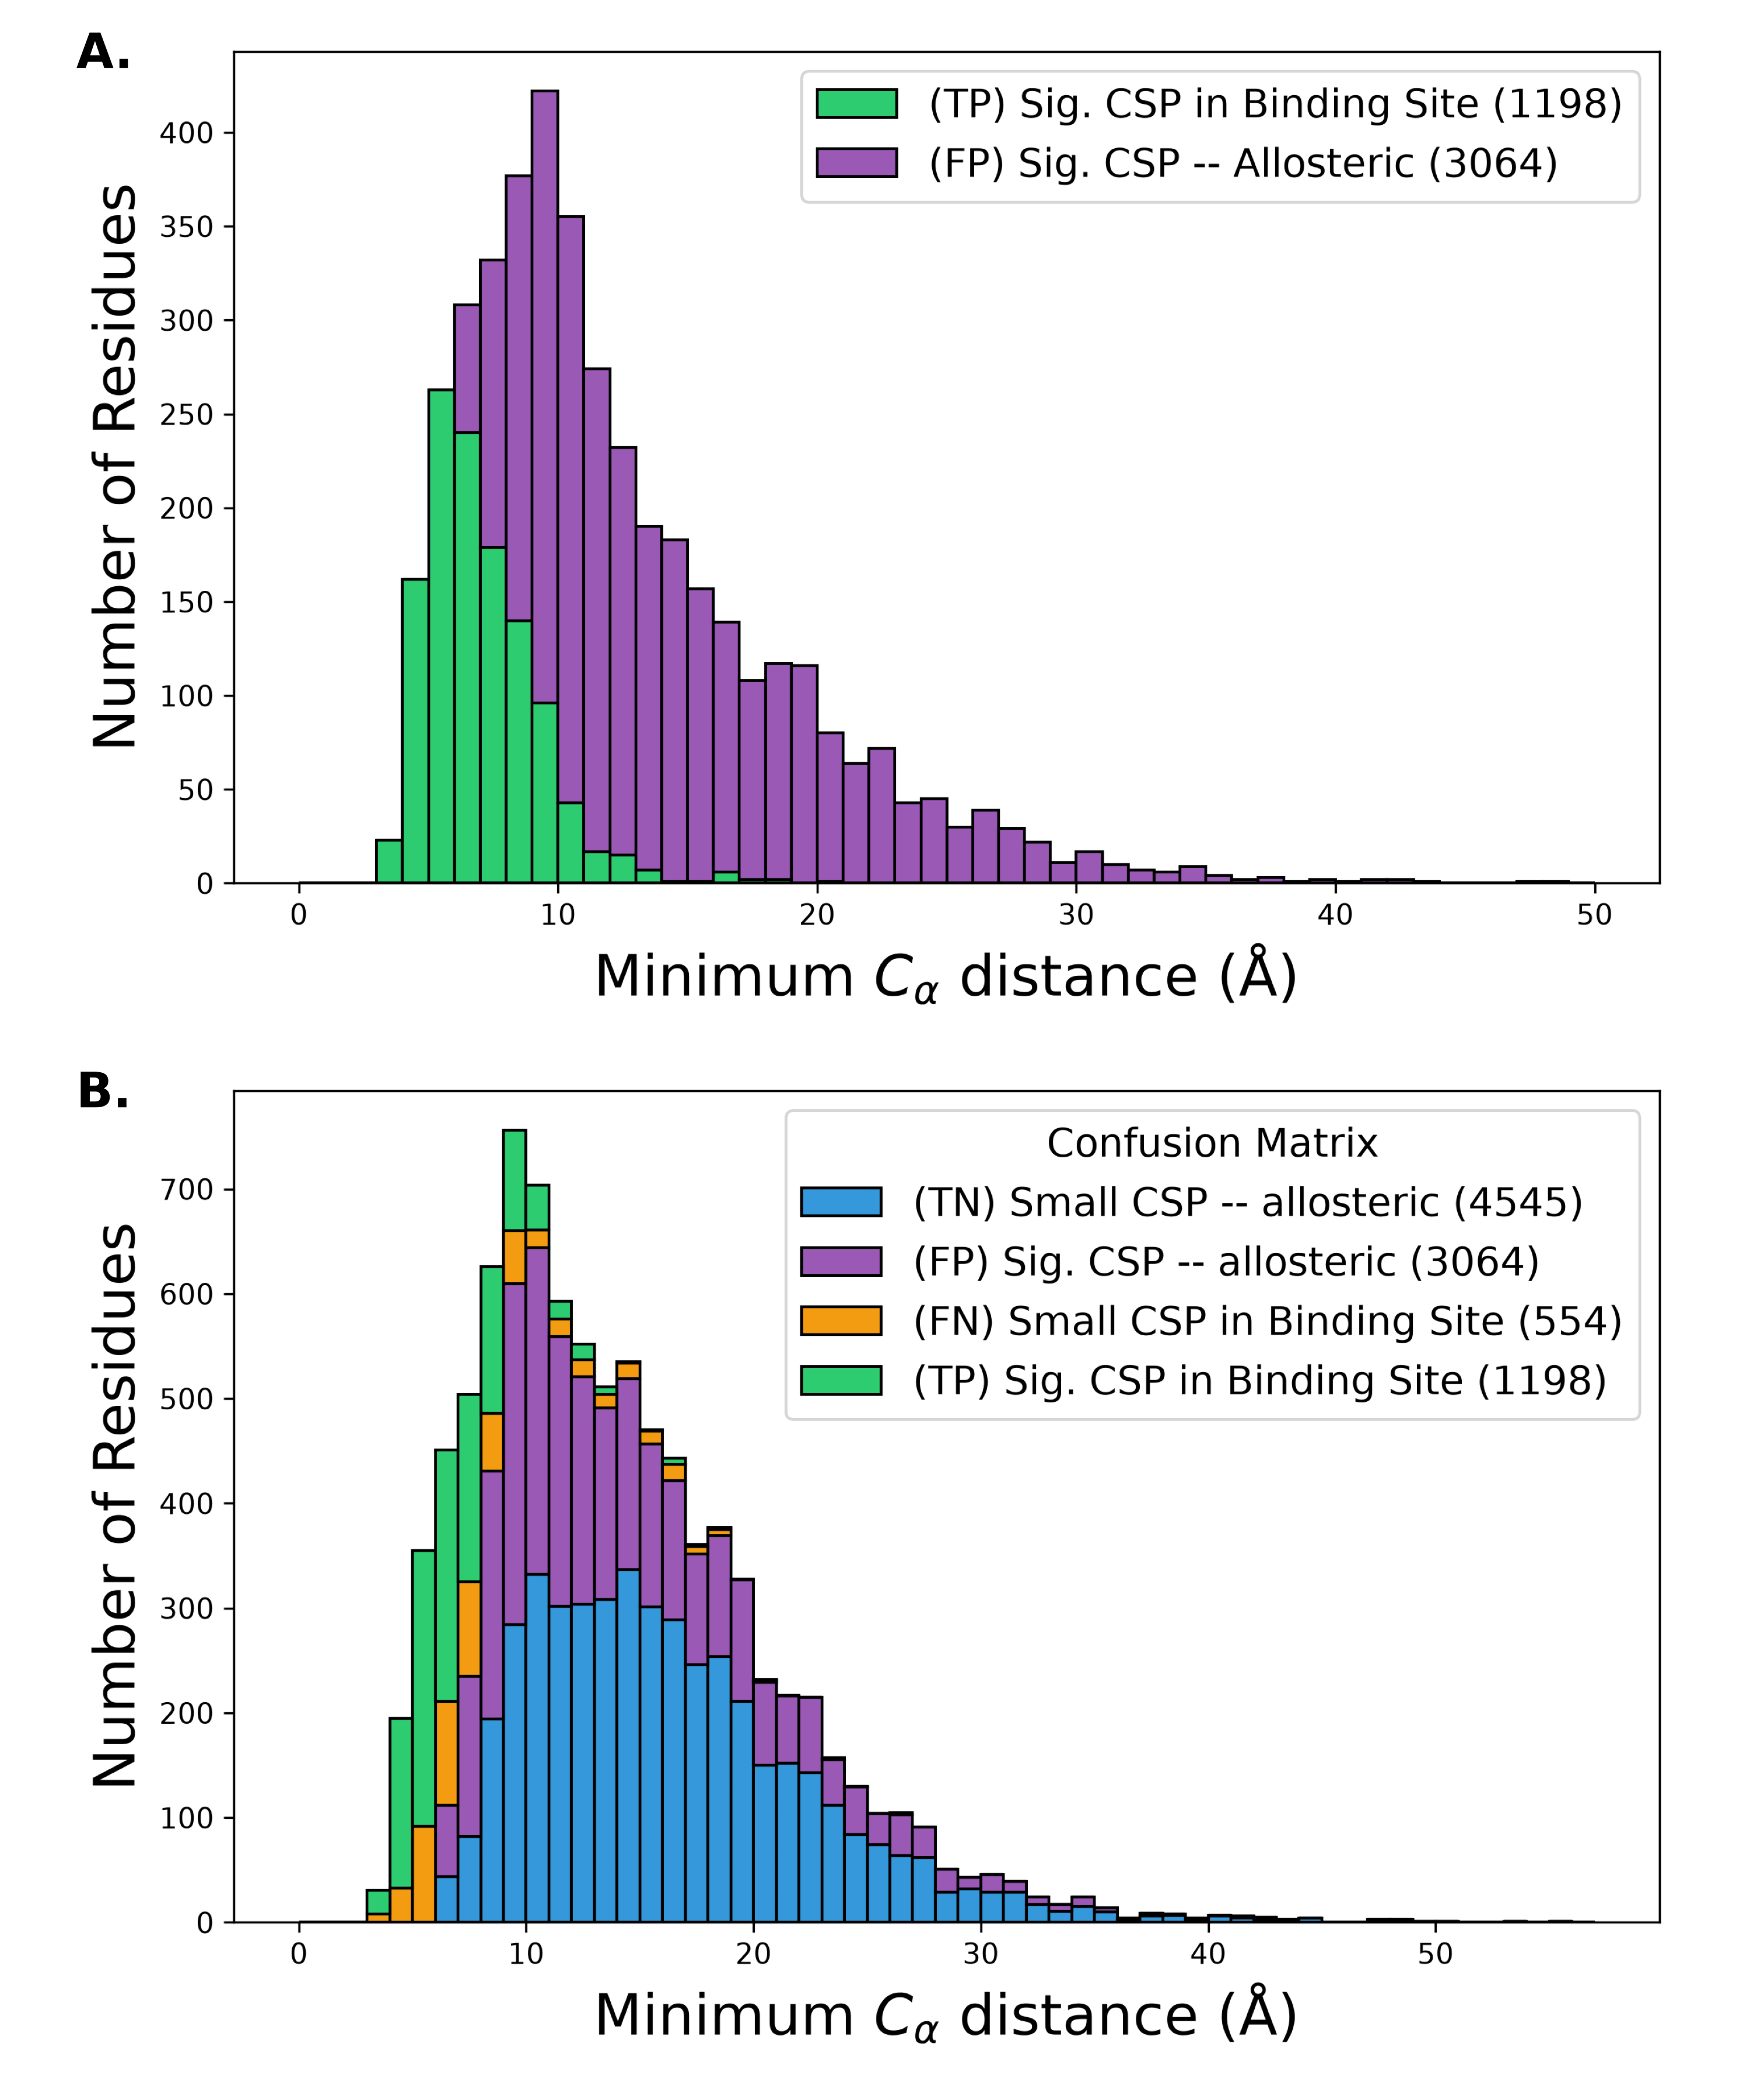
\includegraphics[width=\linewidth]{SF9_ha_ca.png}
\captionsetup{labelformat=empty}
\caption{\textbf{SI Fig. S9. HA/CA CSP confusion histograms} for the
buffer-similar systems from \texttt{CSP\_UBQ\_ph0.5\_temp5C.csv} that also have
H$\alpha$ and C$\alpha$ shifts in both apo and holo experiments ($n=101$).}
\end{figure}

\begin{figure}[H]
\centering
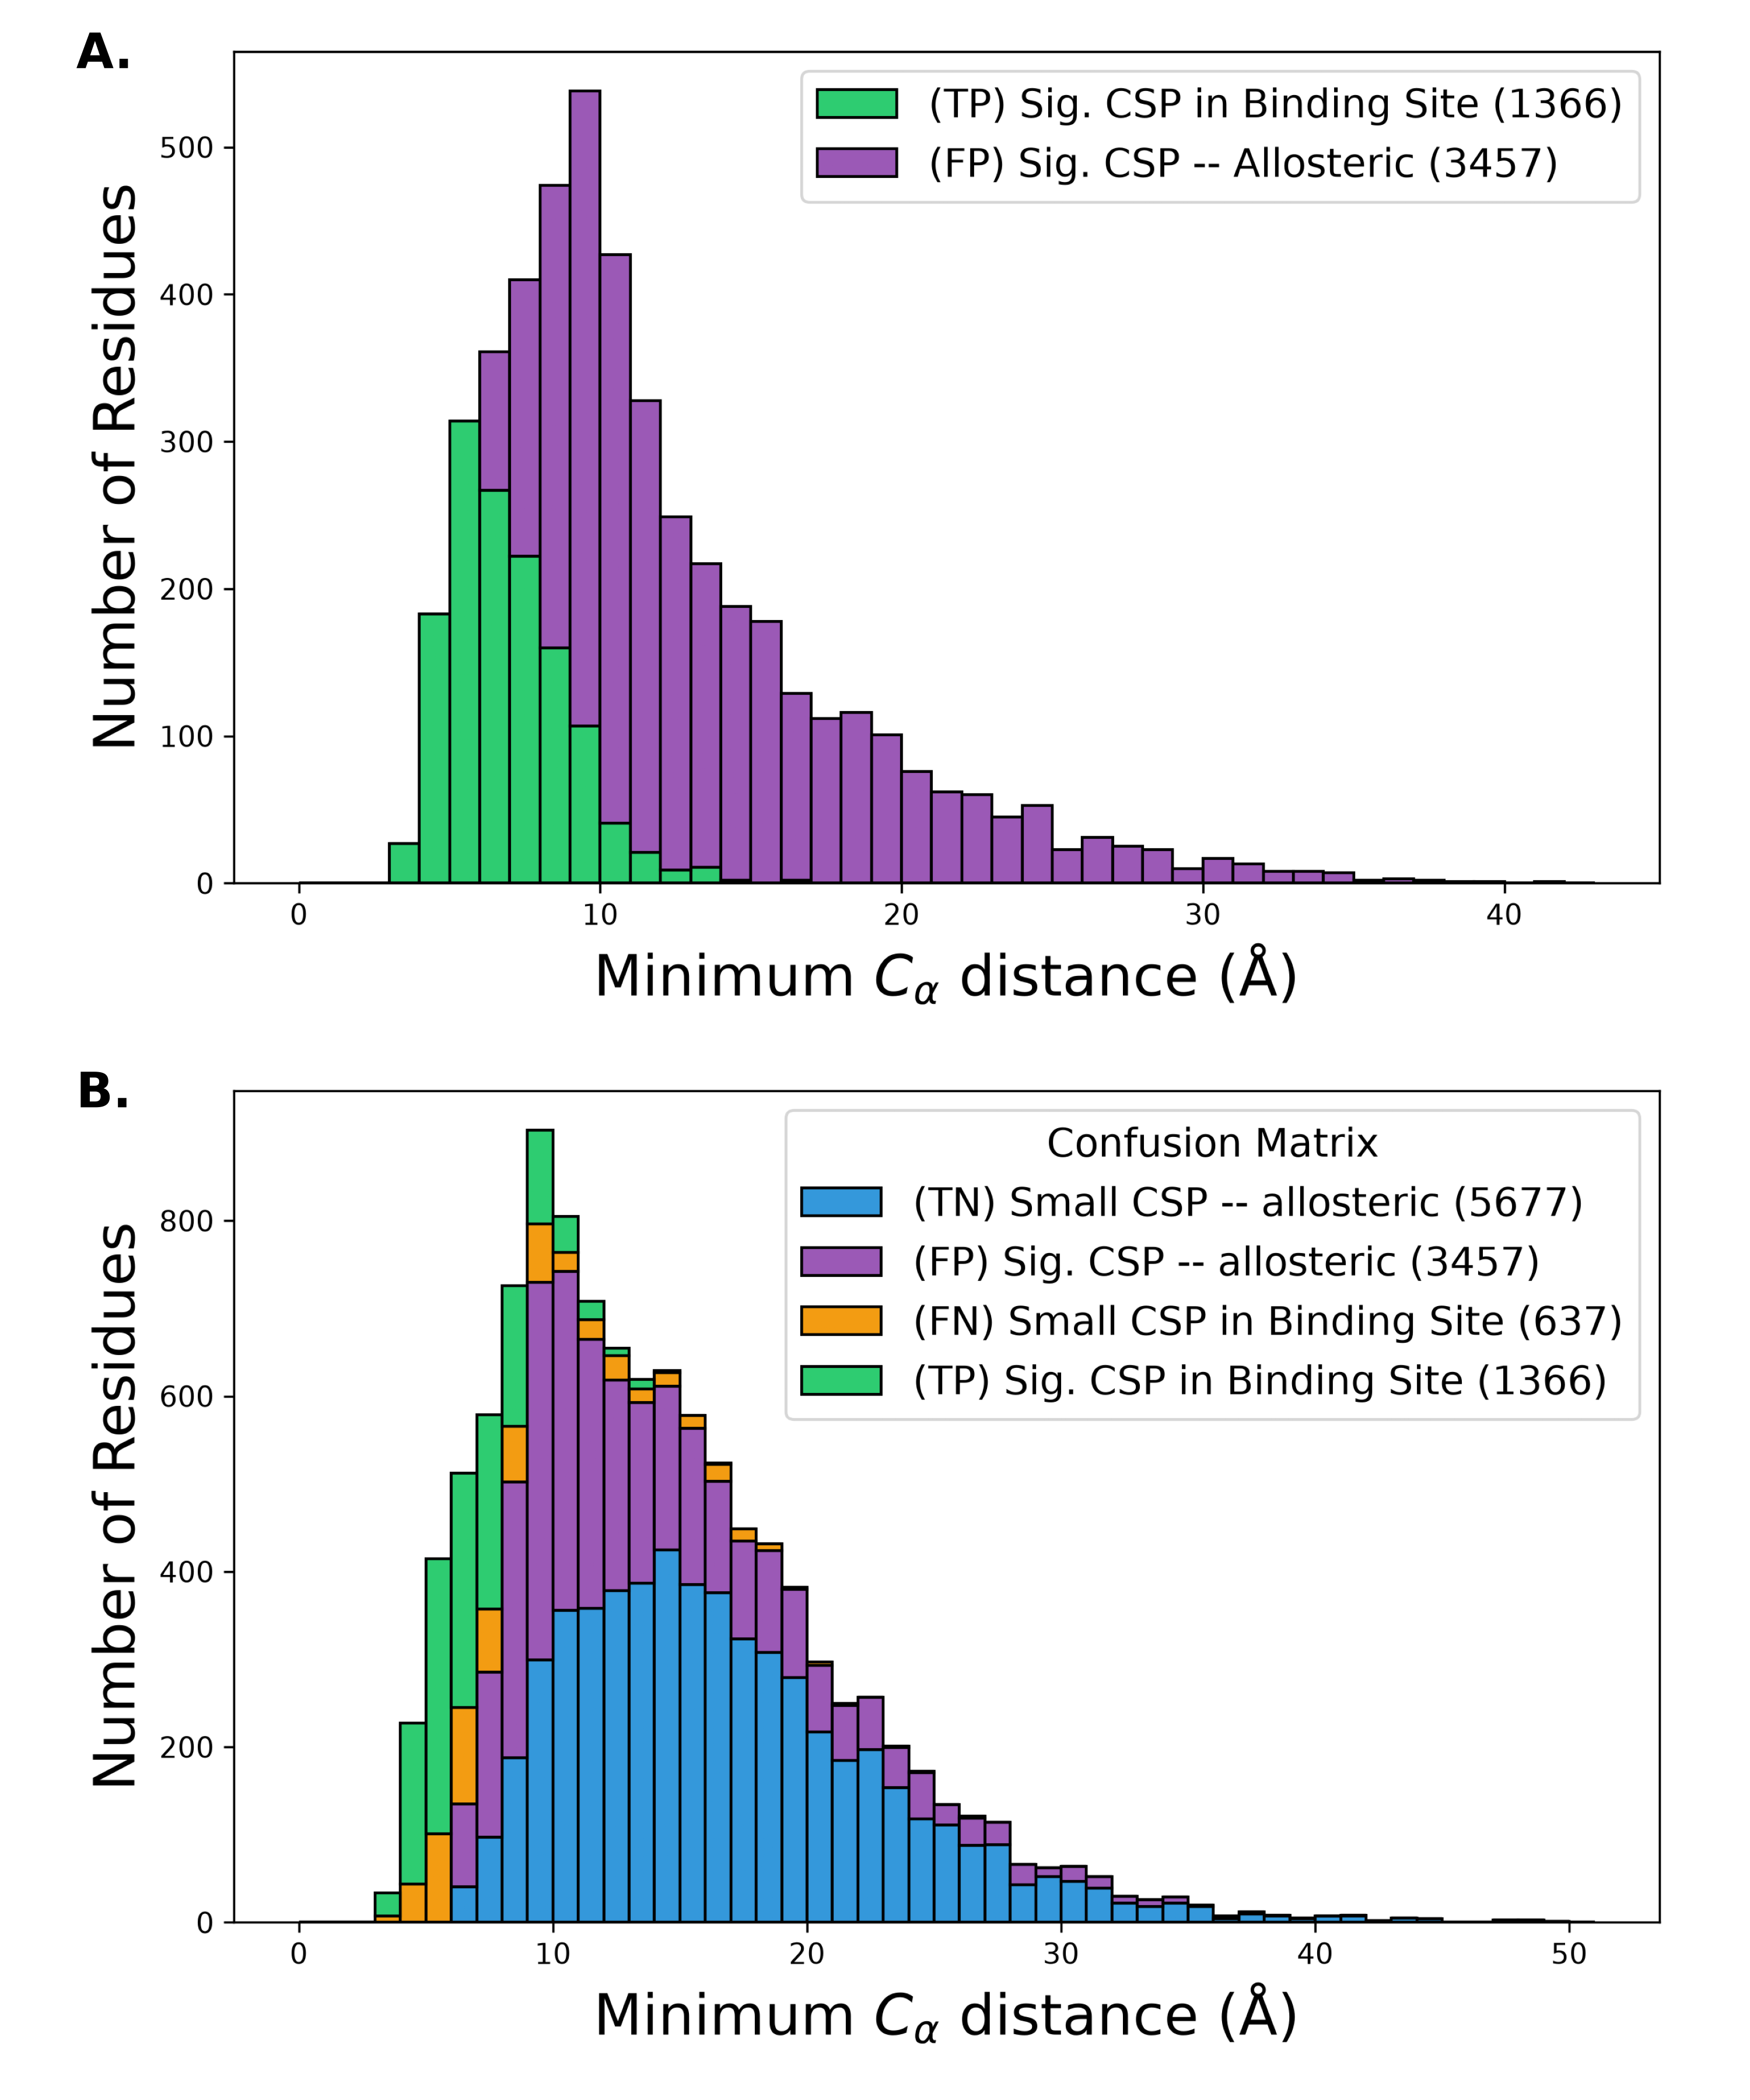
\includegraphics[width=\linewidth]{SF10_ca_inclusive.png}
\captionsetup{labelformat=empty}
\caption{\textbf{SI Fig. S10. CA-inclusive CSP confusion histograms} for the
$n=121$ buffer-similar systems from \texttt{CSP\_UBQ\_ph0.5\_temp5C.csv}
with CA row coverage $>50\%$.}
\end{figure}

\begin{figure}[H]
\centering
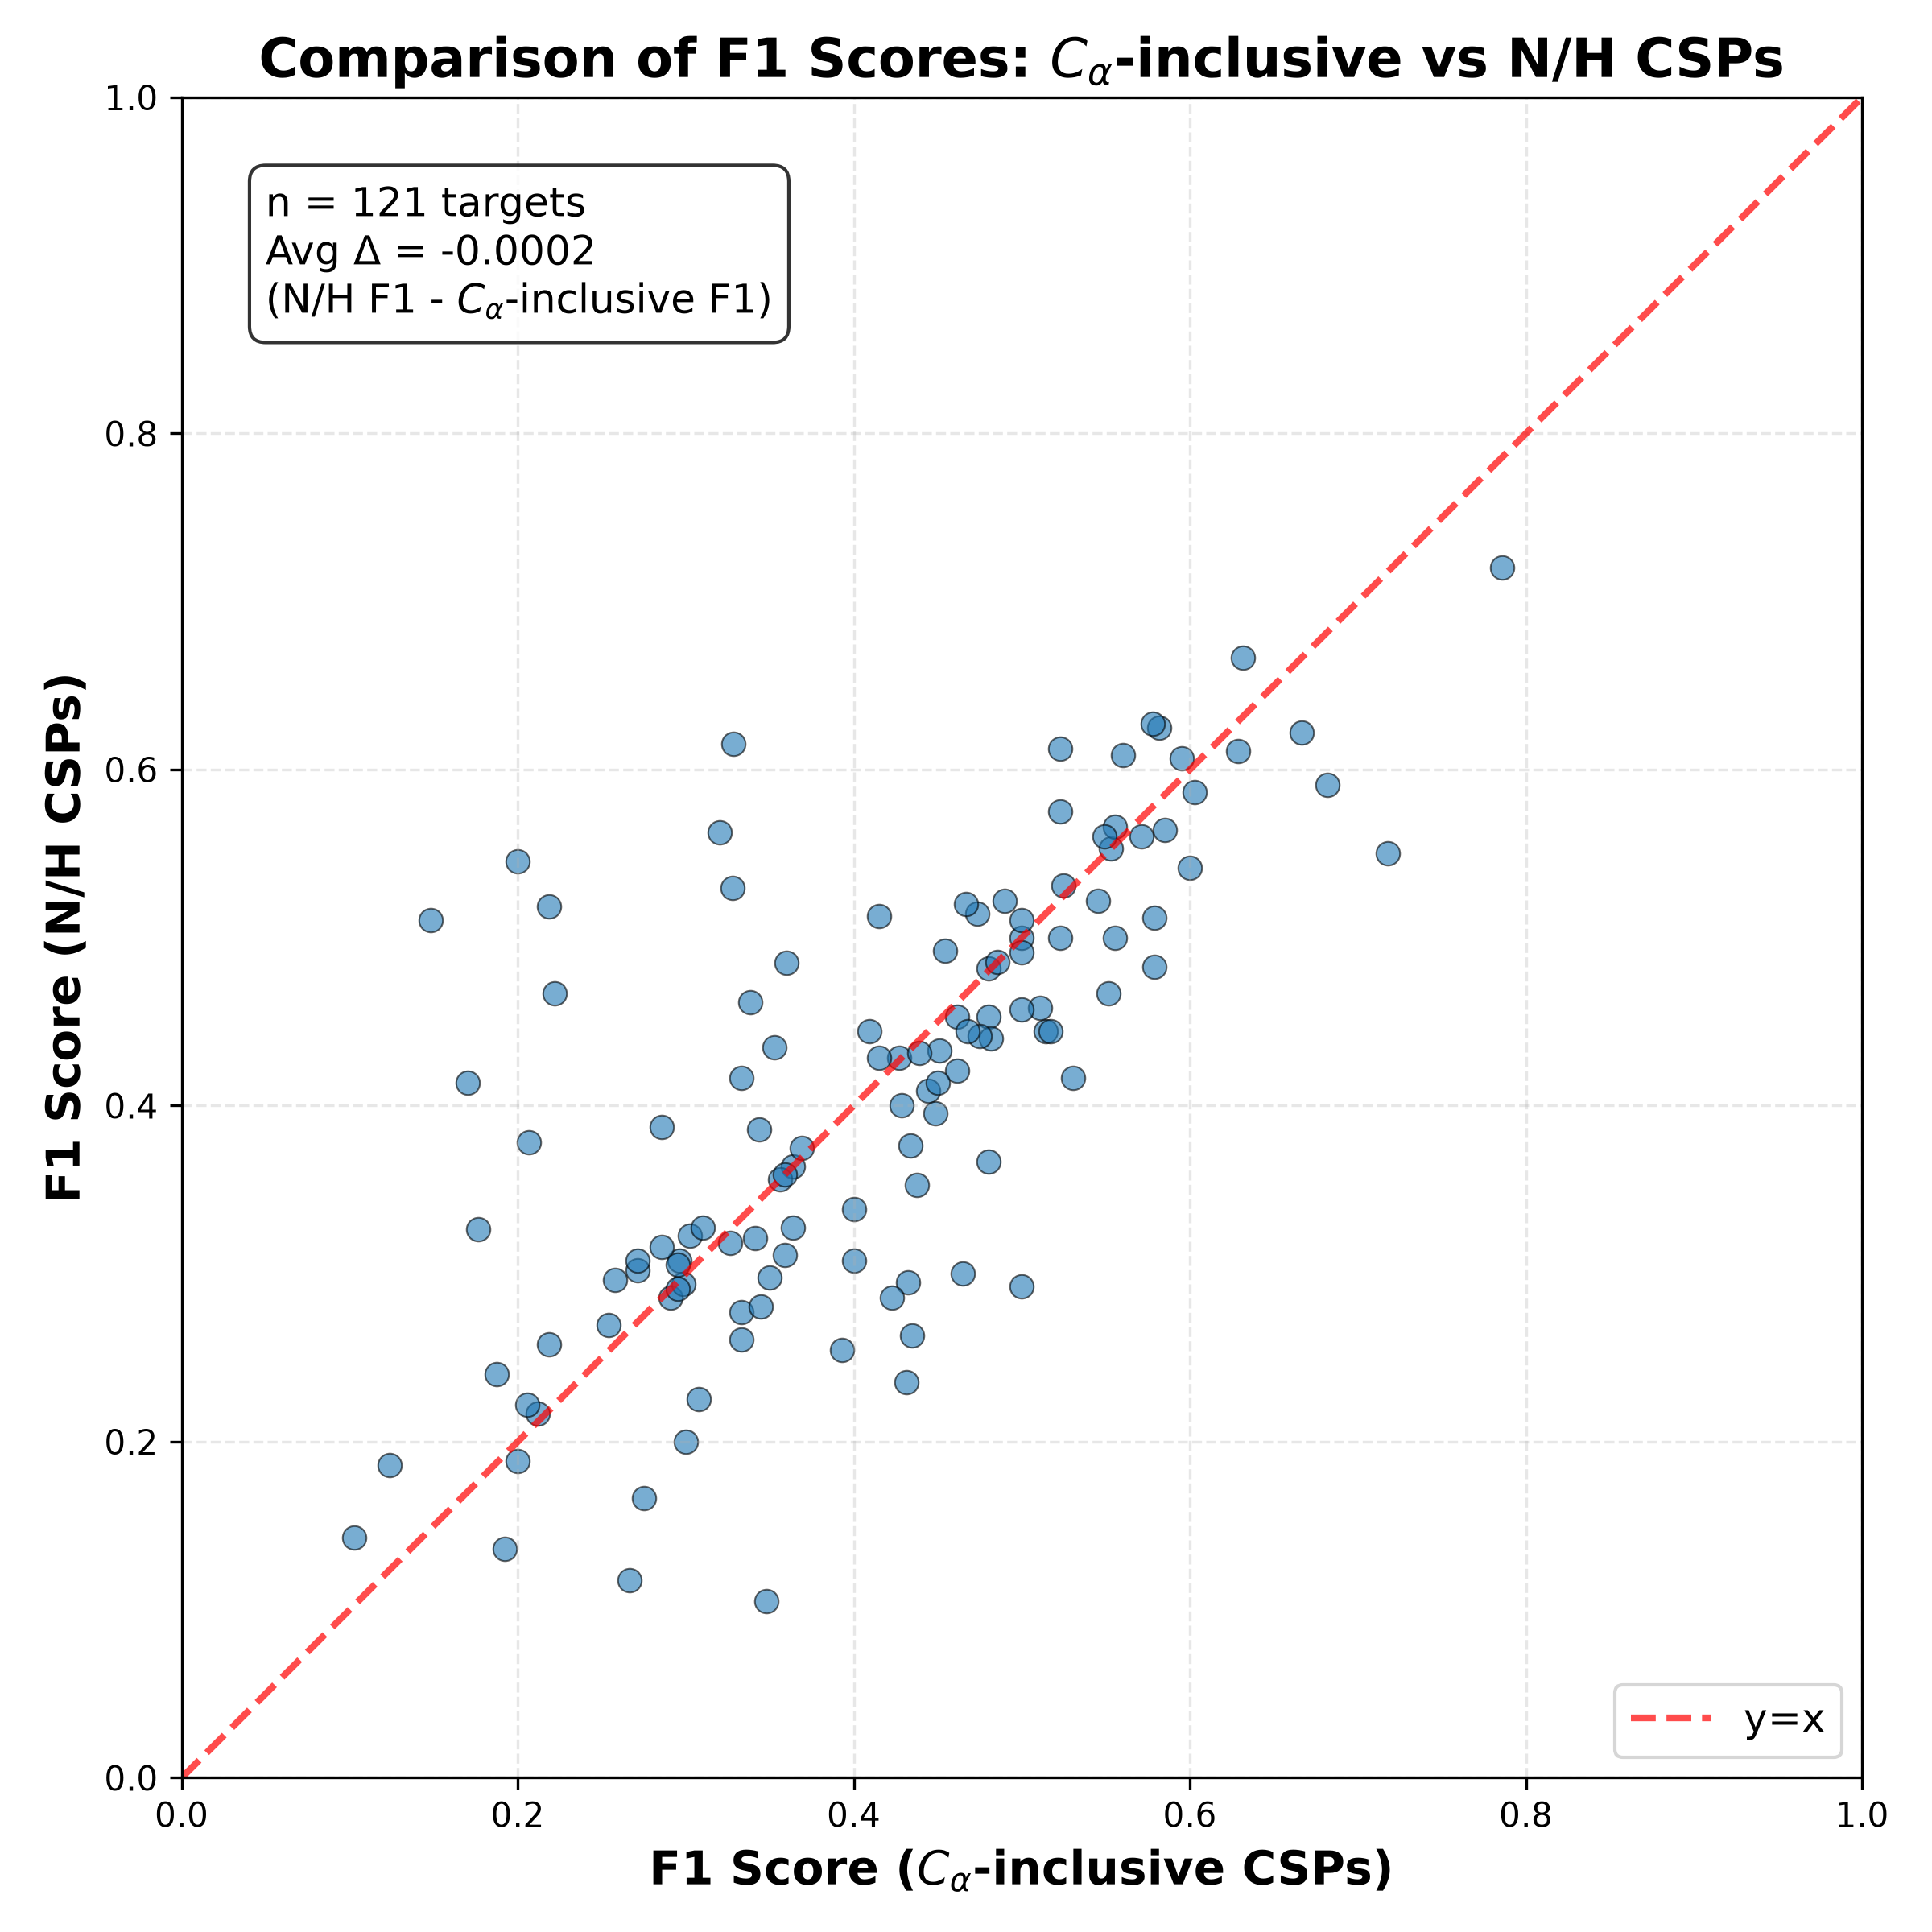
\includegraphics[width=0.95\linewidth]{SF11_f1_ca_vs_exclusive.png}
\captionsetup{labelformat=empty}
\caption{\textbf{SI Fig. S11. F1 scores for CA-inclusive vs exclusive CSPs}
($n=121$ buffer-similar systems from \texttt{CSP\_UBQ\_ph0.5\_temp5C.csv}
with CA row coverage $>50\%$).}
\end{figure}

\begin{figure}[H]
\centering
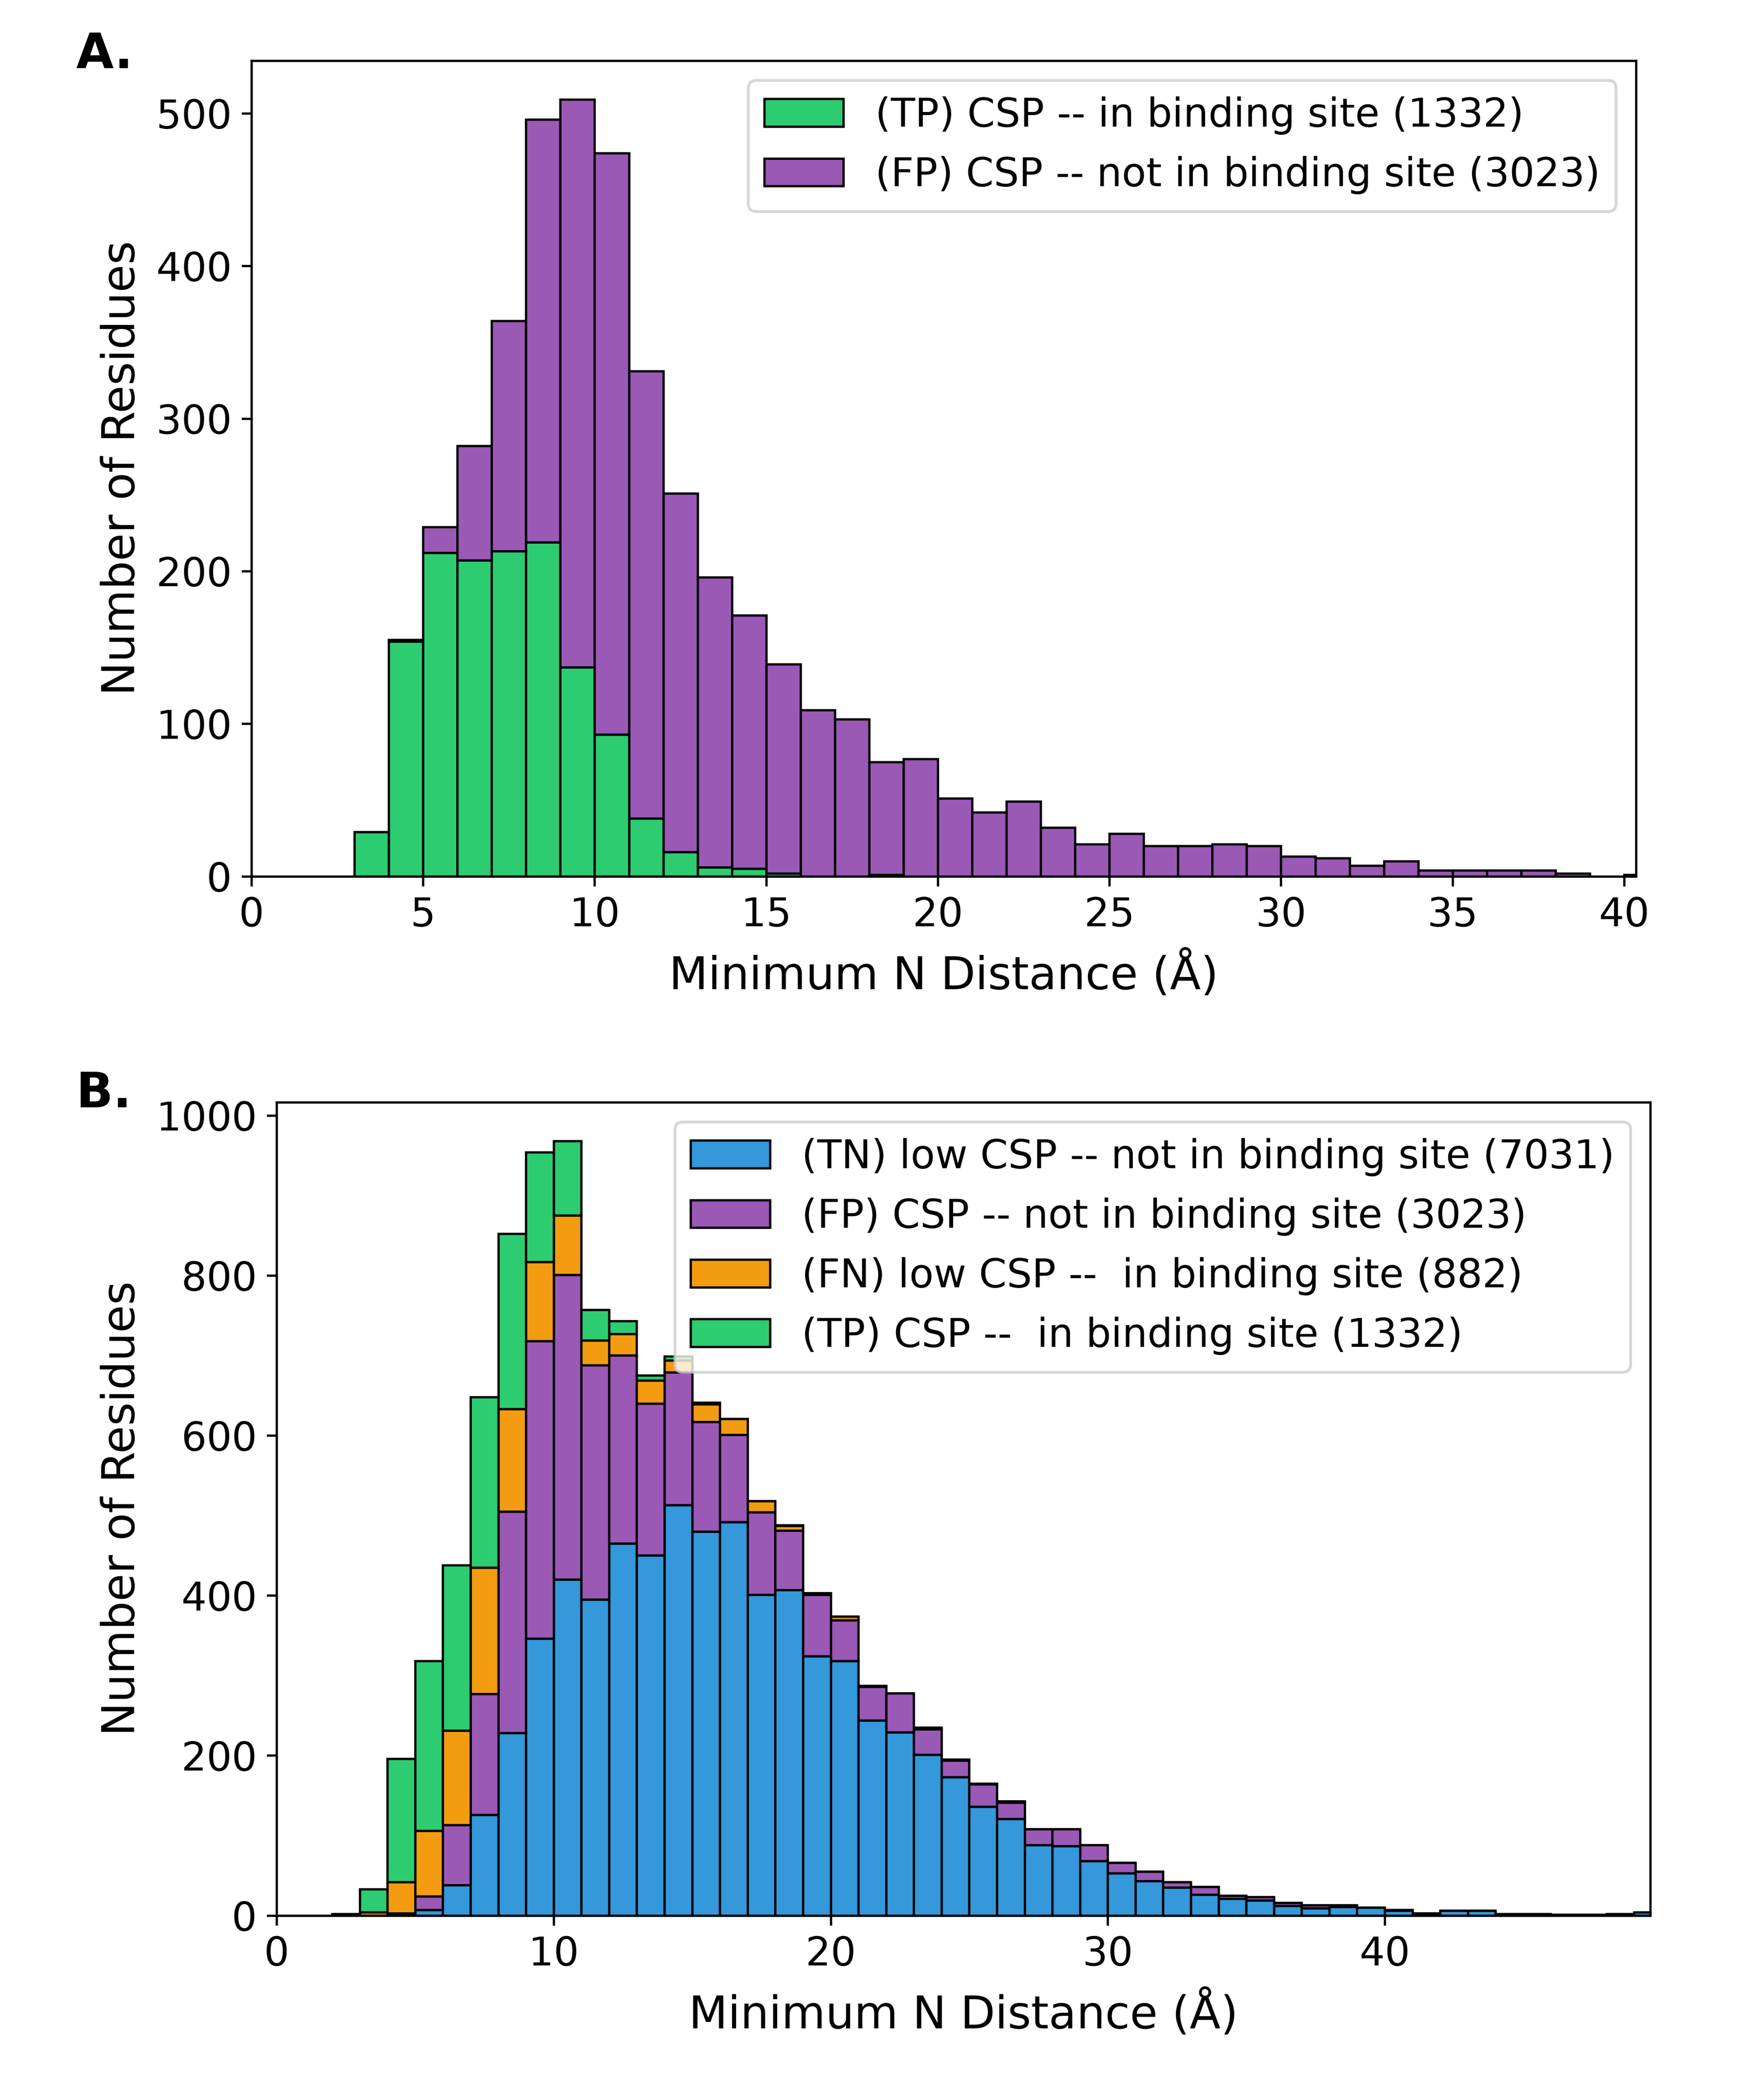
\includegraphics[width=\linewidth]{SF12_nn_distance.png}
\captionsetup{labelformat=empty}
\caption{\textbf{SI Fig. S12. Confusion histograms by closest interchain N--N distance}
($n=135$ buffer-similar systems from \texttt{CSP\_UBQ\_ph0.5\_temp5C.csv}
with pipeline outputs).}
\end{figure}

\begin{figure}[H]
\centering
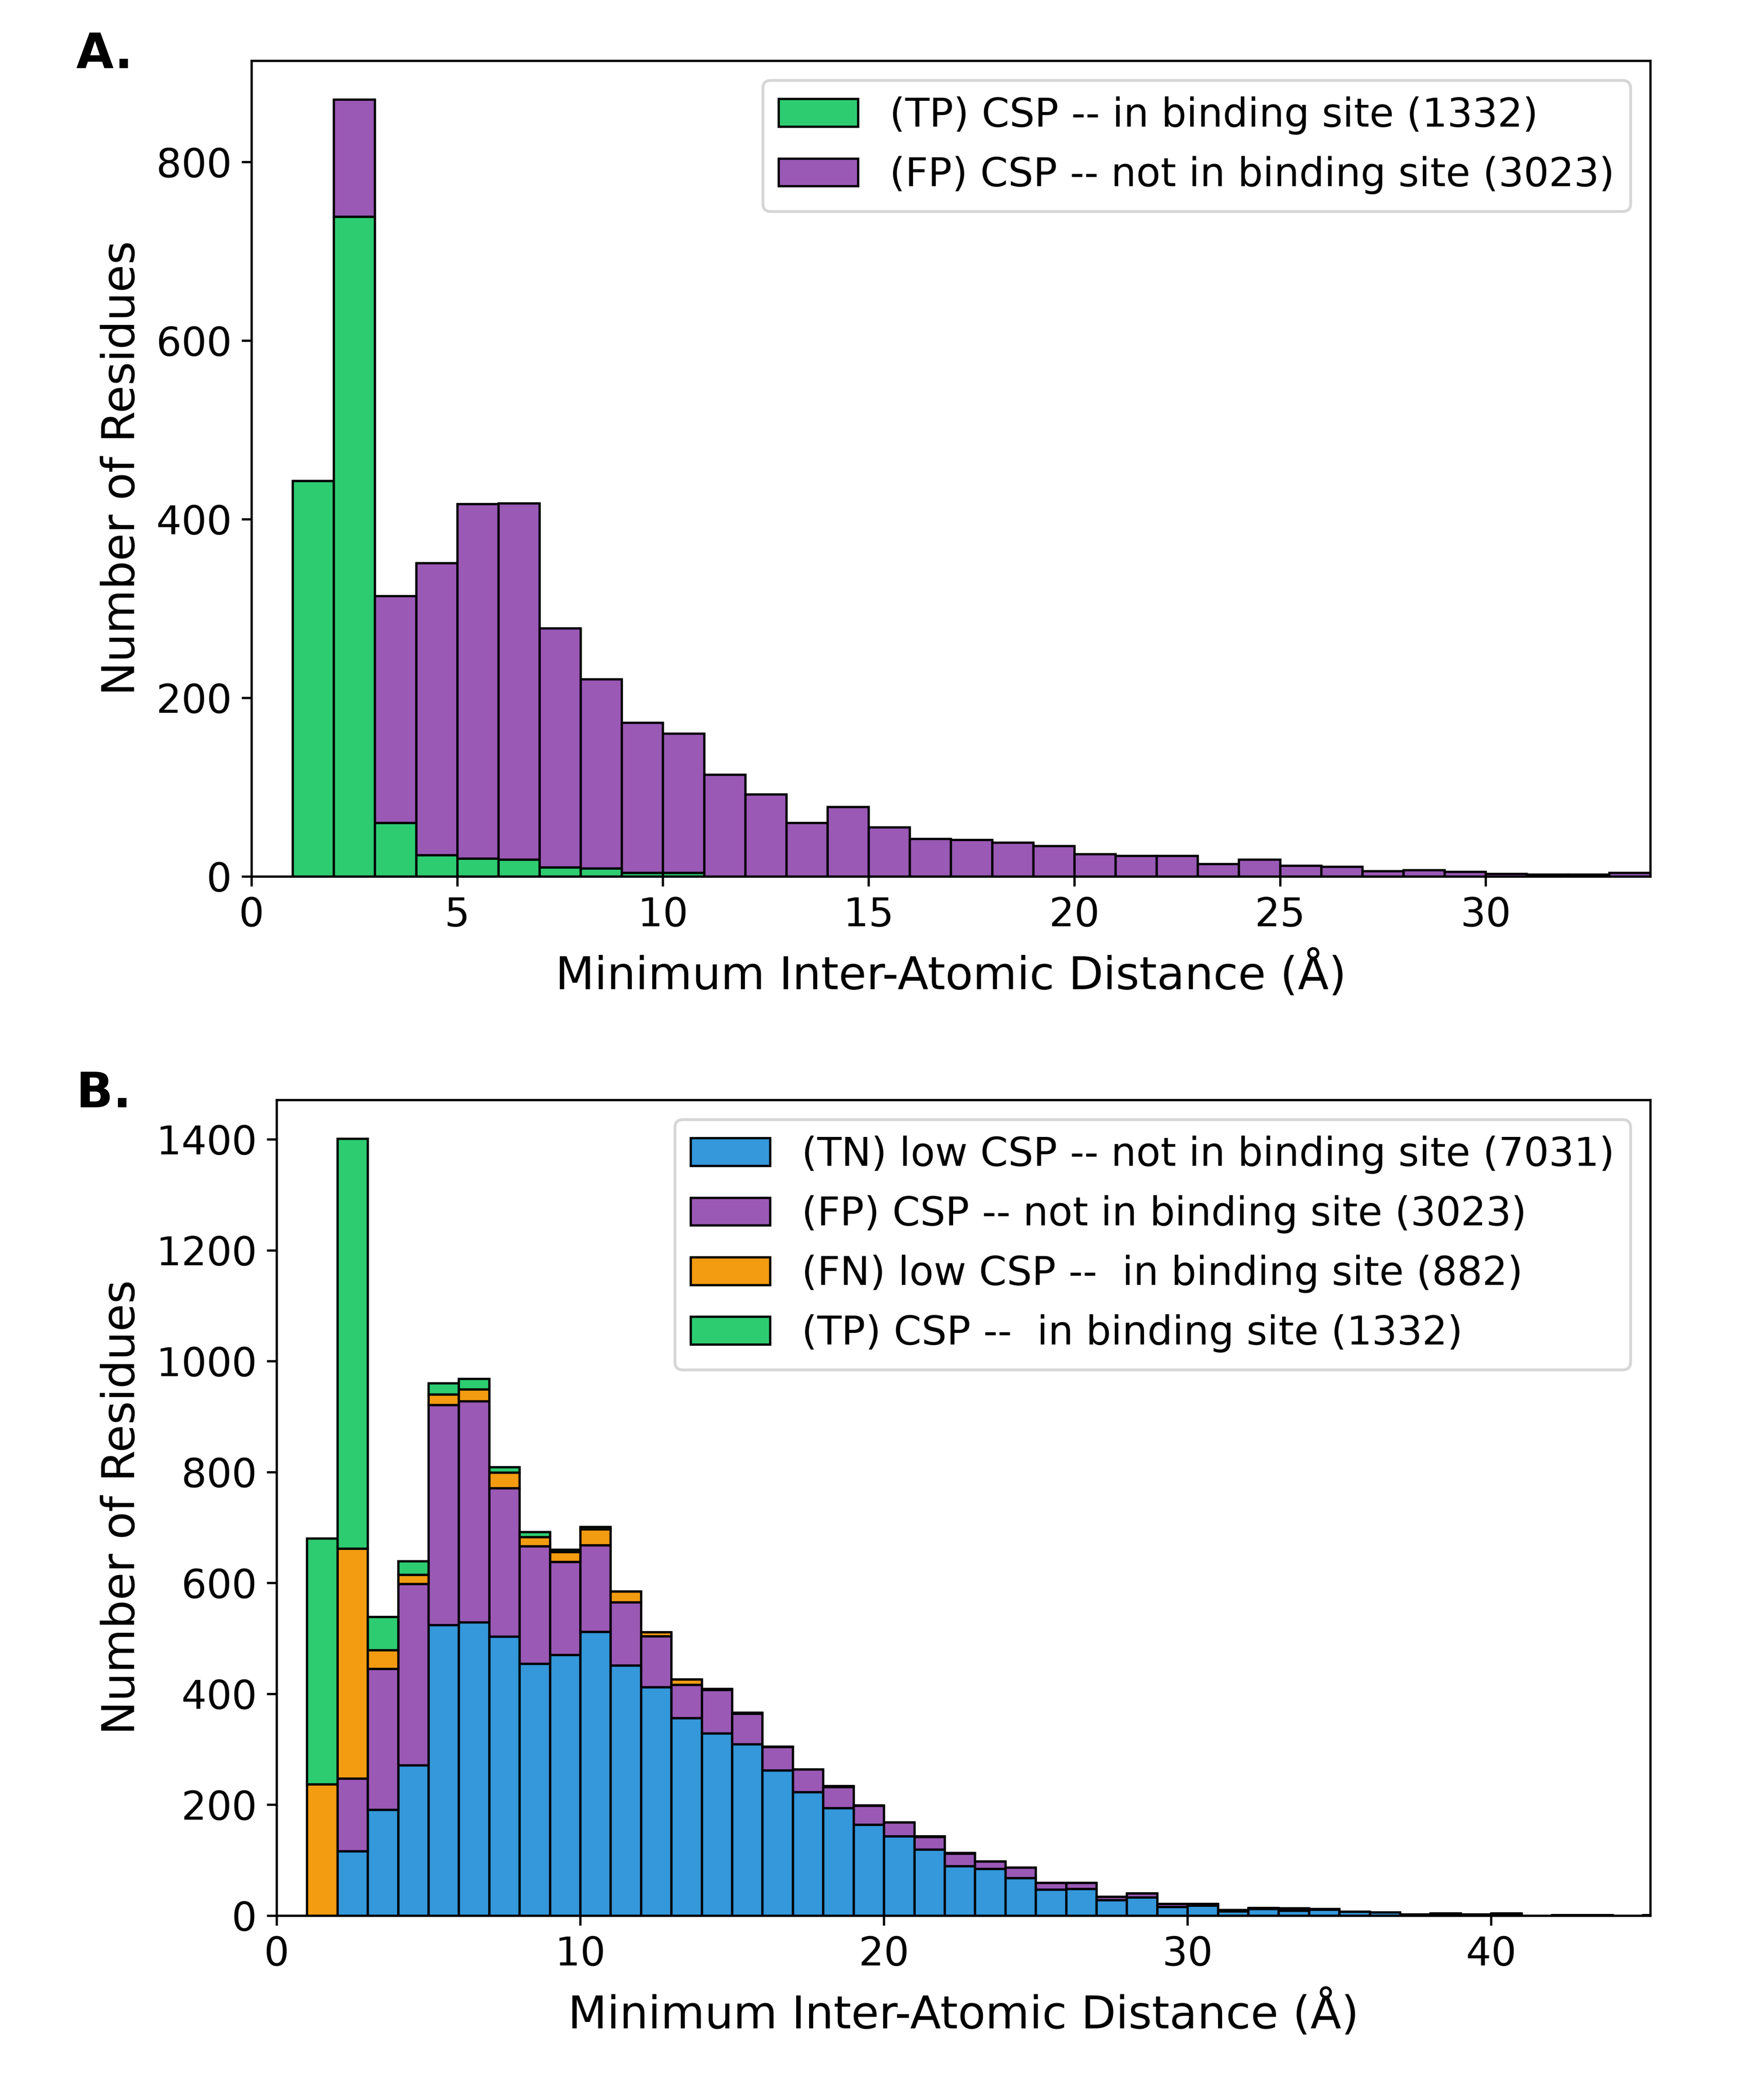
\includegraphics[width=\linewidth]{SF13_any_atom_distance.png}
\captionsetup{labelformat=empty}
\caption{\textbf{SI Fig. S13. Confusion histograms by closest interchain any-atom distance}
($n=135$ buffer-similar systems from \texttt{CSP\_UBQ\_ph0.5\_temp5C.csv}
with pipeline outputs).}
\end{figure}

\begin{figure}[H]
\centering
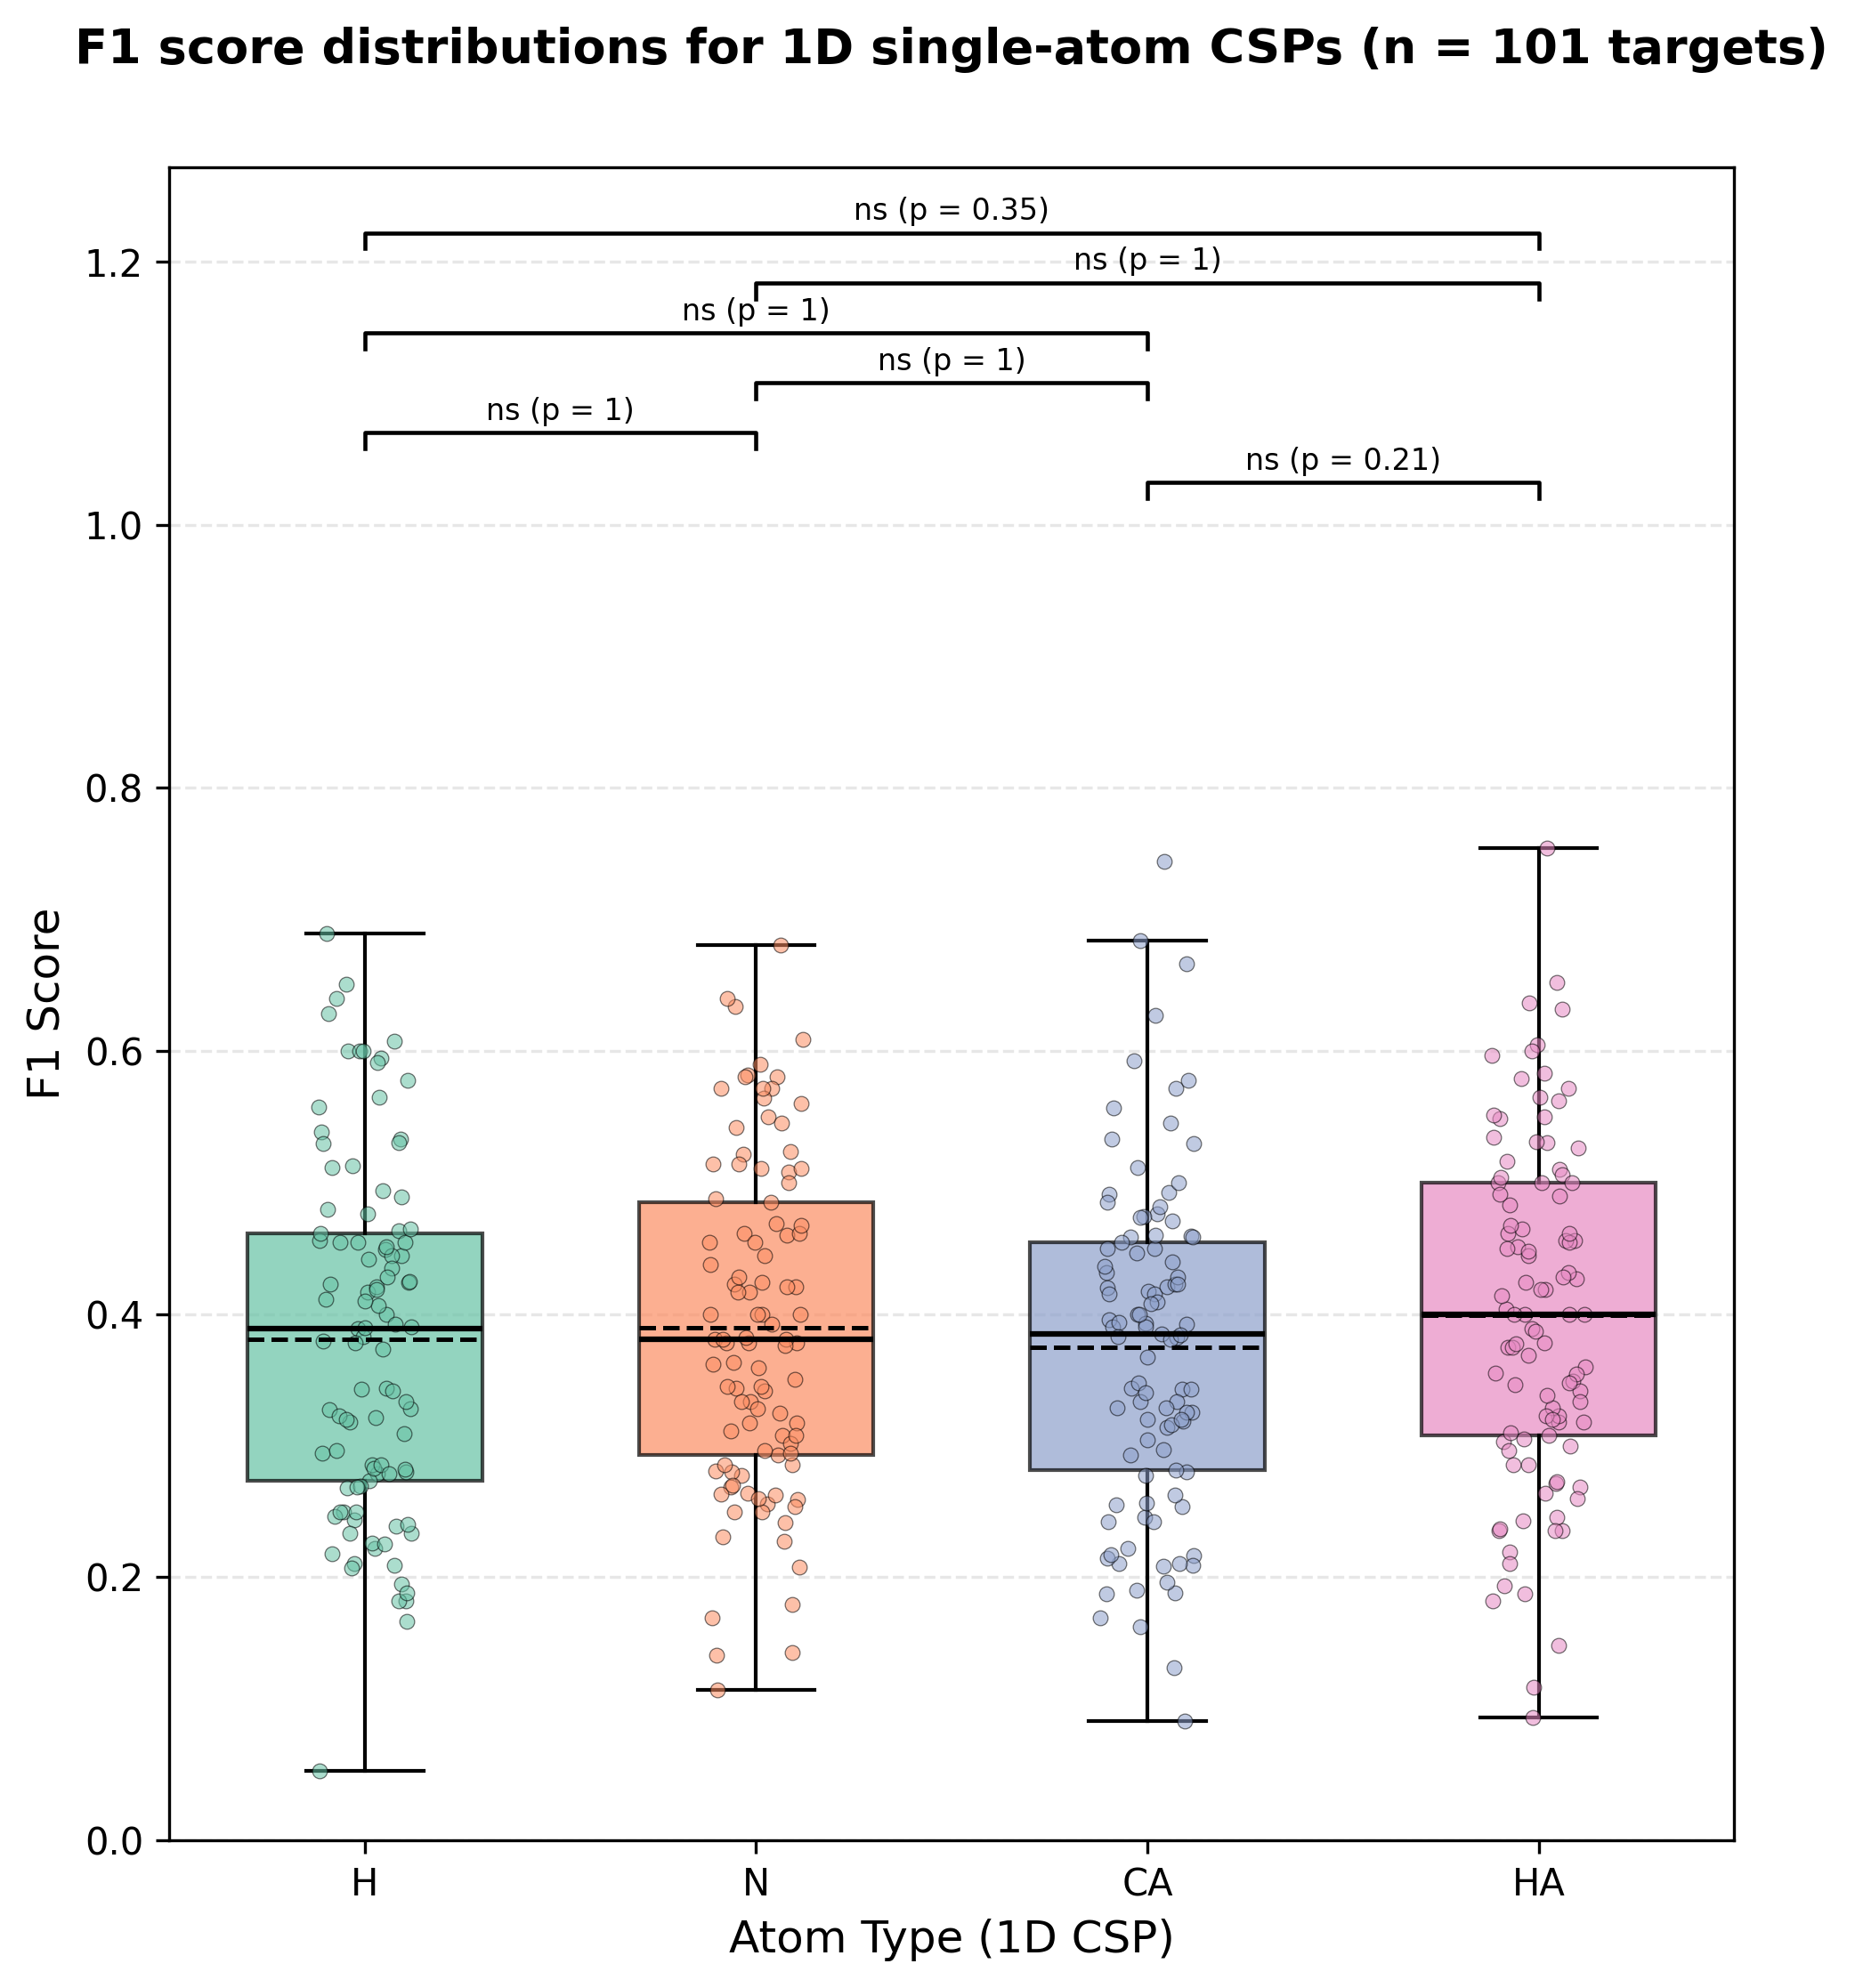
\includegraphics[width=0.9\linewidth]{SF14_1d_CSP_boxplot.png}
\captionsetup{labelformat=empty}
\caption{\textbf{SI Fig. S14. Per-target F1 scores for 1D H/N/C$\alpha$/H$\alpha$ CSPs}
($n=101$ buffer-similar systems from \texttt{CSP\_UBQ\_ph0.5\_temp5C.csv}
with paired H/N/CA/HA F1 scores).
Boxes show the per-target F1 distribution for 1D CSPs of each nucleus.
Pairwise comparisons are two-sided Wilcoxon signed-rank tests for all unordered
atom pairs, with Holm--Bonferroni adjustment of $p$-values.}
\end{figure}

\begin{figure}[H]
\centering
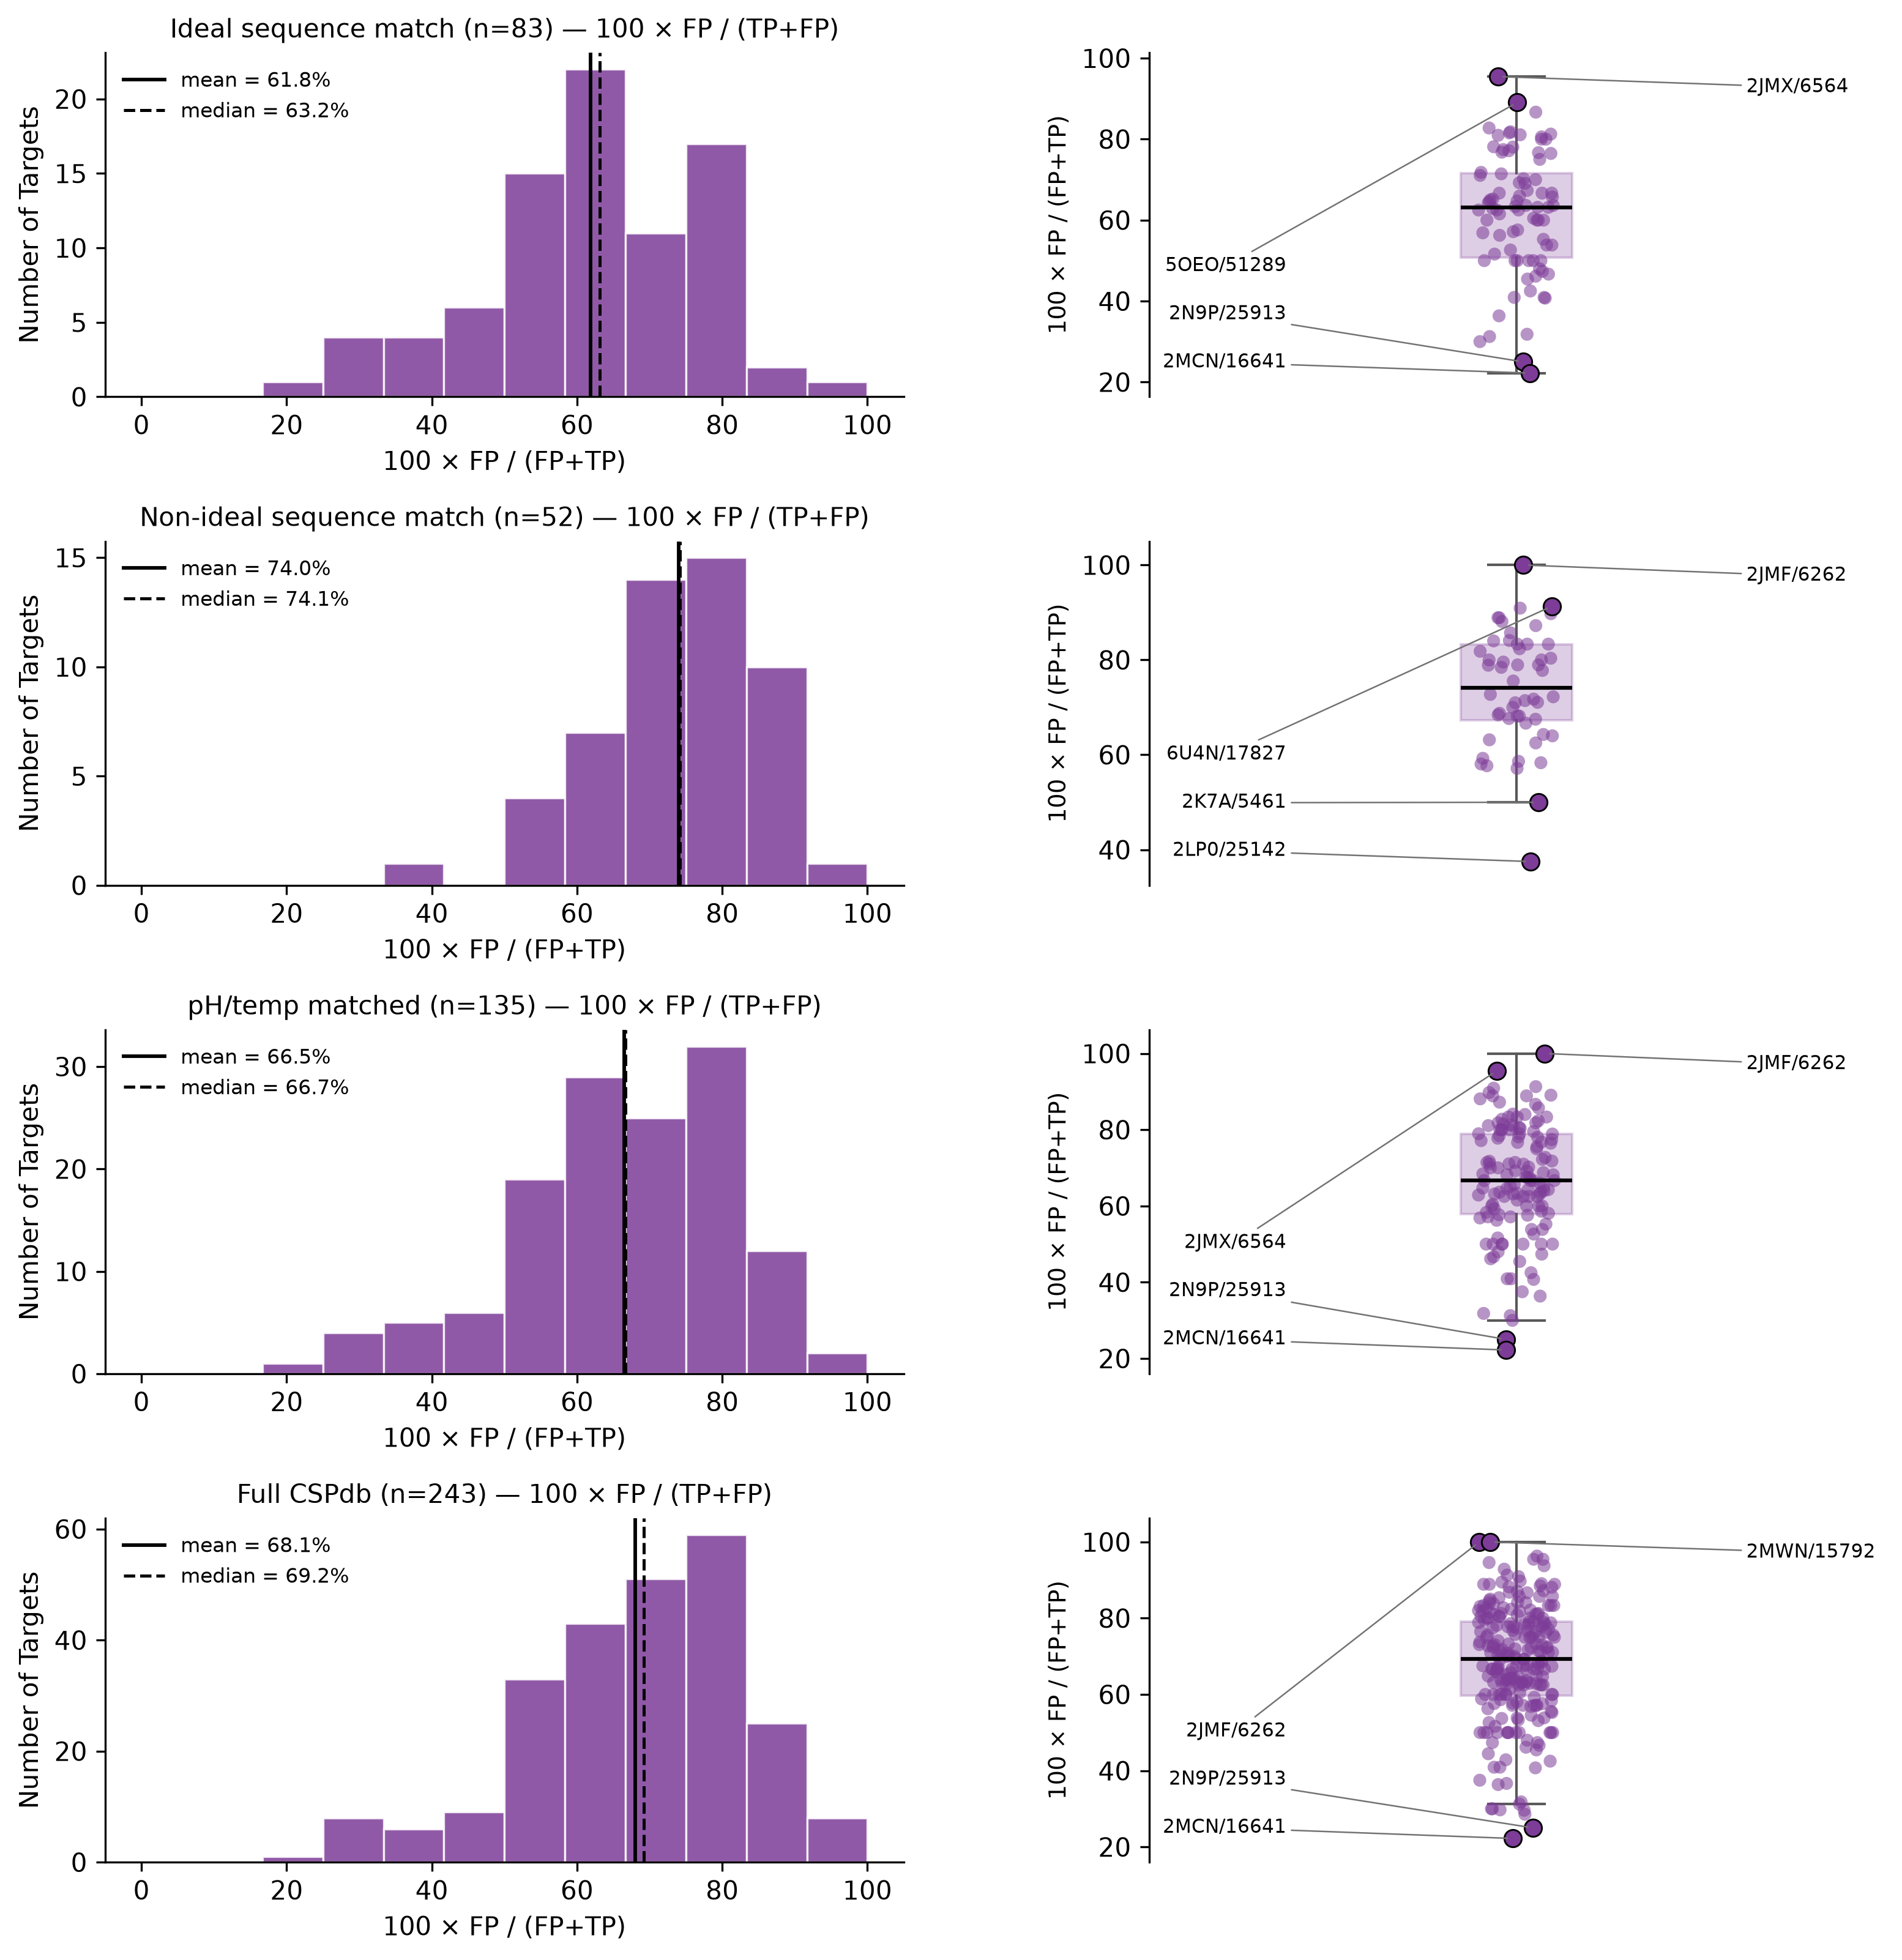
\includegraphics[width=0.95\linewidth]{SF15_fp_percent_distribution_cleaned_mean.png}
\captionsetup{labelformat=empty}
\caption{\textbf{SI Fig. S15. Per-target false-positive rates} under the primary CSP
cutoff $\max(\text{cleaned mean},\,0.05\,\mathrm{ppm})$.
Rows show four cohorts:
\textbf{ideal sequence match} ($n=83$),
\textbf{non-ideal sequence match} ($n=52$),
\textbf{pH/temp matched} ($n=135$),
and the \textbf{full CSPdb} ($n=243$).
For each cohort, panels report
$100\times\mathrm{FP}/(\mathrm{TP}+\mathrm{FP})$ among significant CSPs.}
\end{figure}

\begin{figure}[H]
\centering
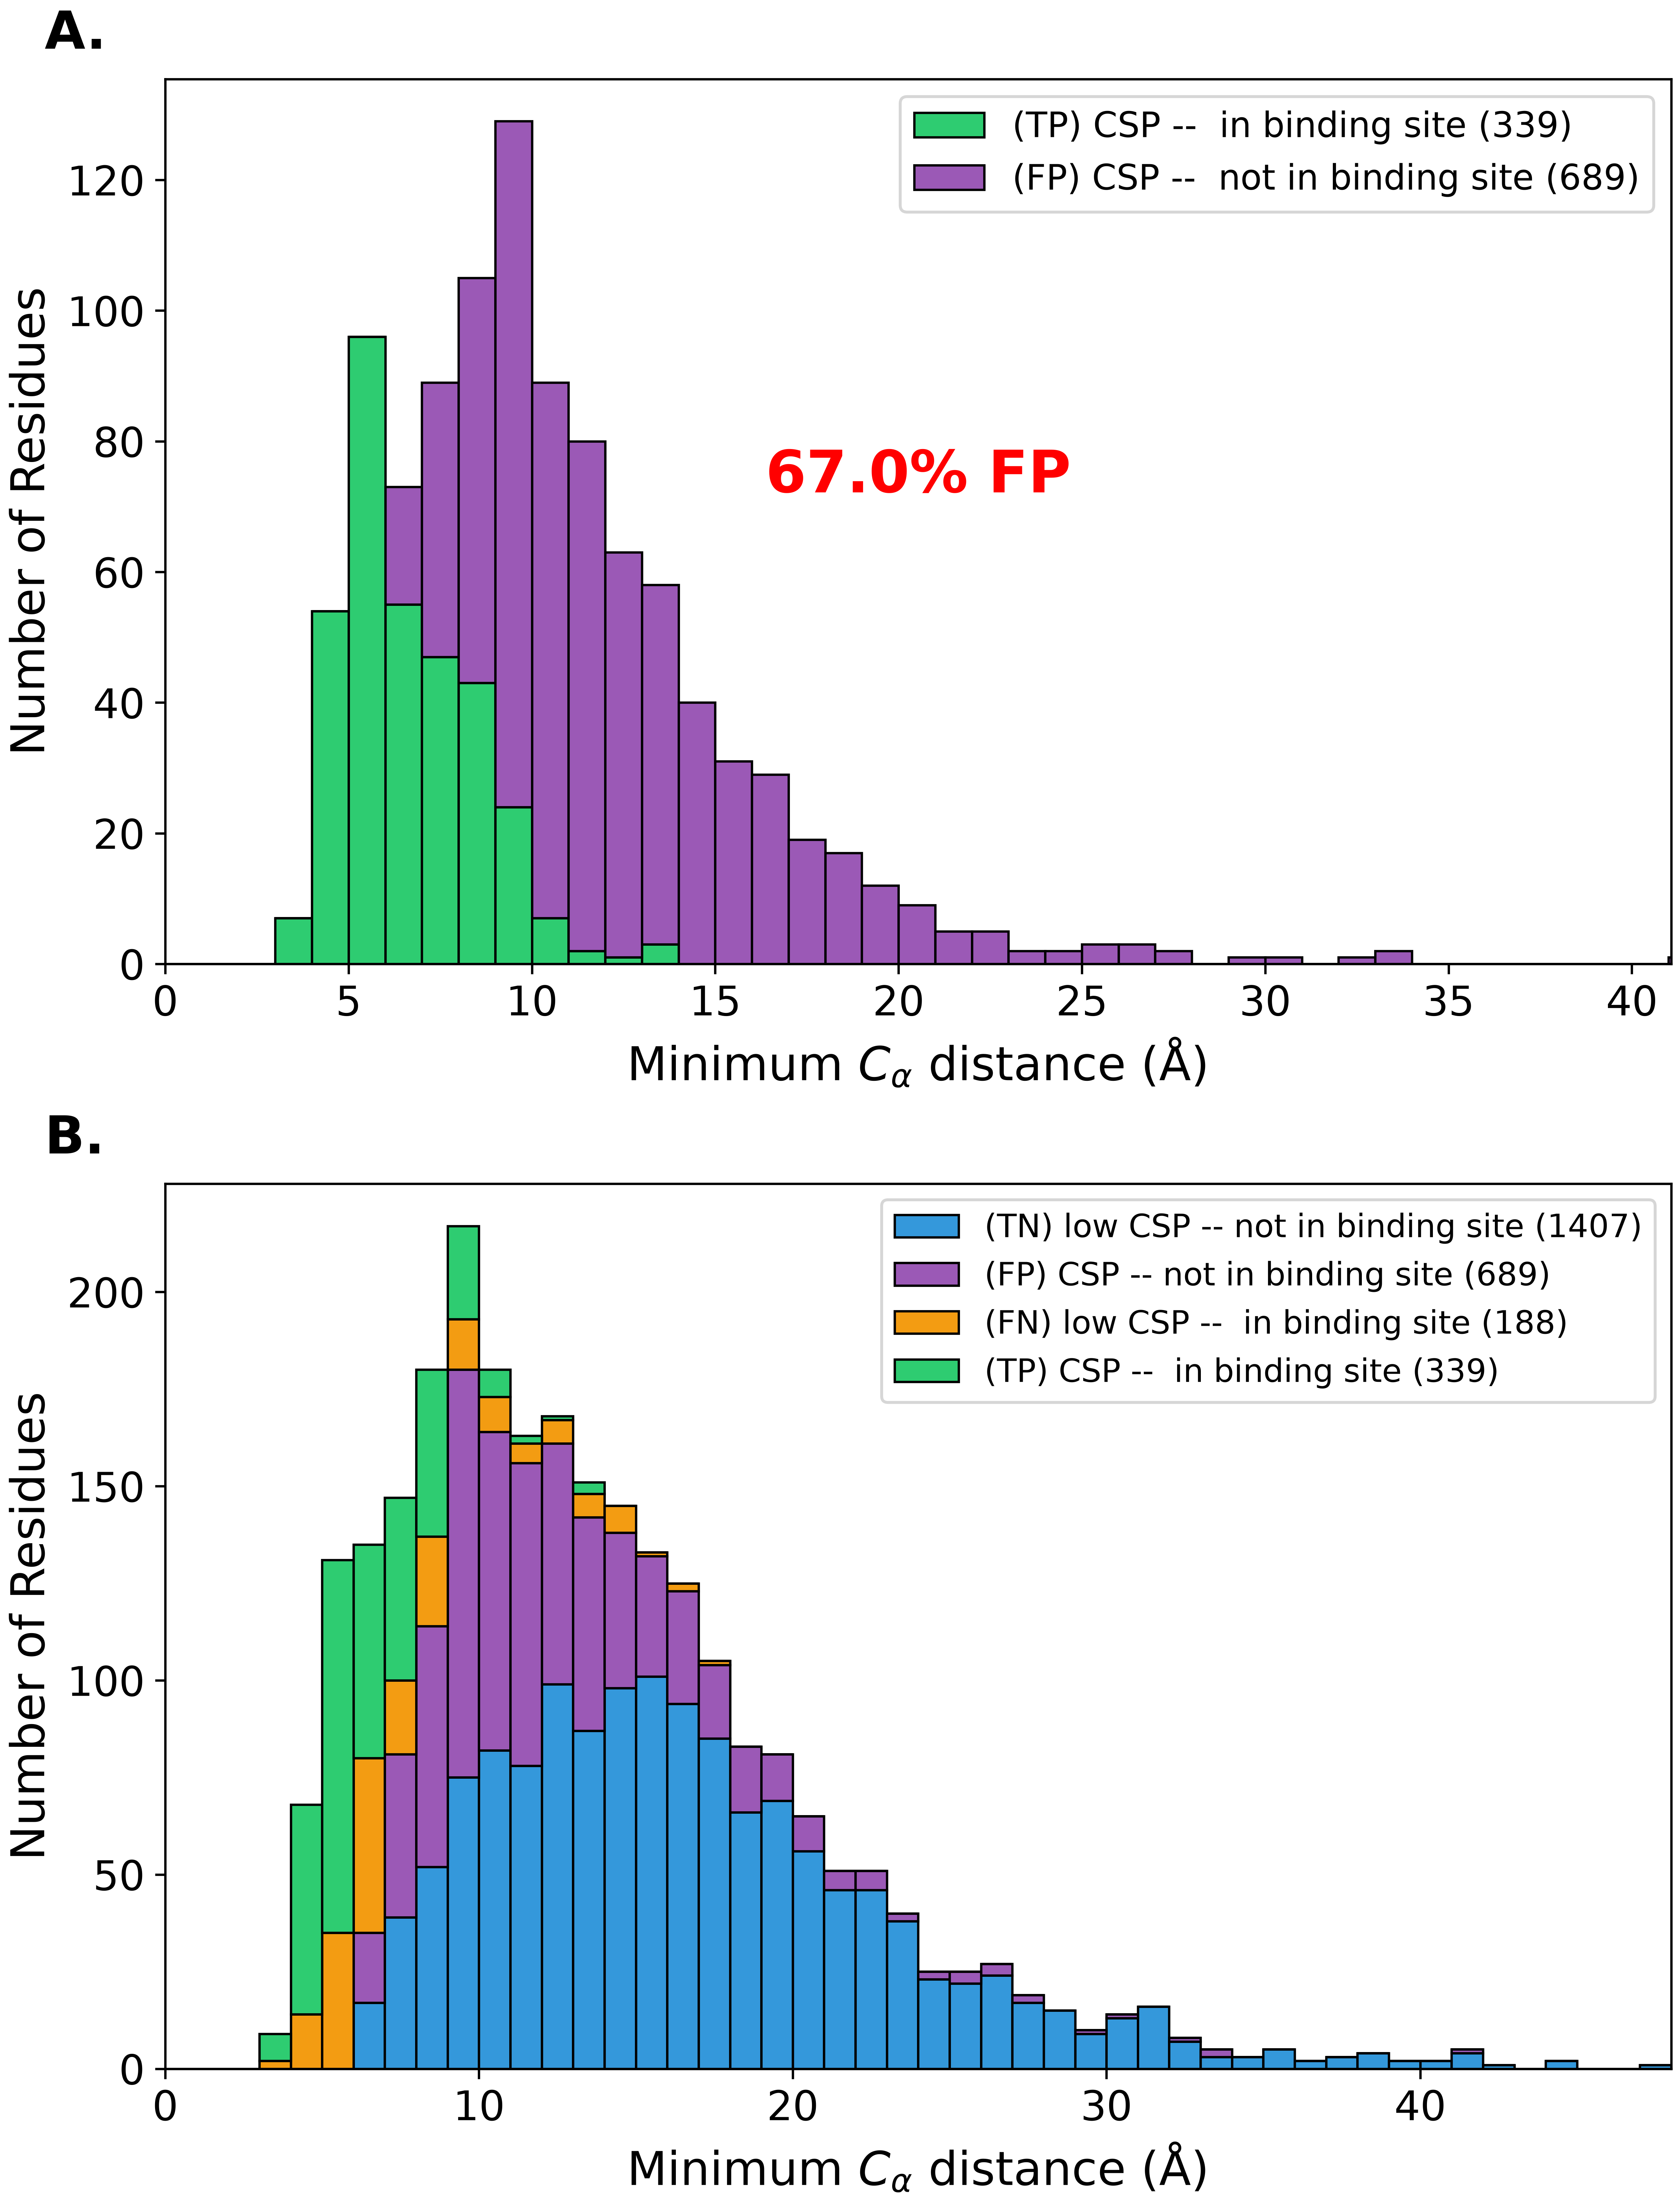
\includegraphics[width=\linewidth]{SF16_figure_3_combined_same_author_list.png}
\captionsetup{labelformat=empty}
\caption{\textbf{SI Fig. S16. Figure~3 histograms for the same-author/same-study subset.}
Targets are the curated pairs in
\texttt{CSP\_UBQ\_ph0.5\_temp5C\_same\_author\_list.csv}
($n=32$ with pipeline outputs of 33 curated pairs): buffer-similar apo/holo systems that share a study or last author
between apo and holo chemical-shift depositions.
Left: significant-CSP TP vs FP by minimum C$\alpha$ distance to the interface;
right: full confusion-matrix stacks (TN/FP/FN/TP).}
\end{figure}

\begin{figure}[H]
\centering
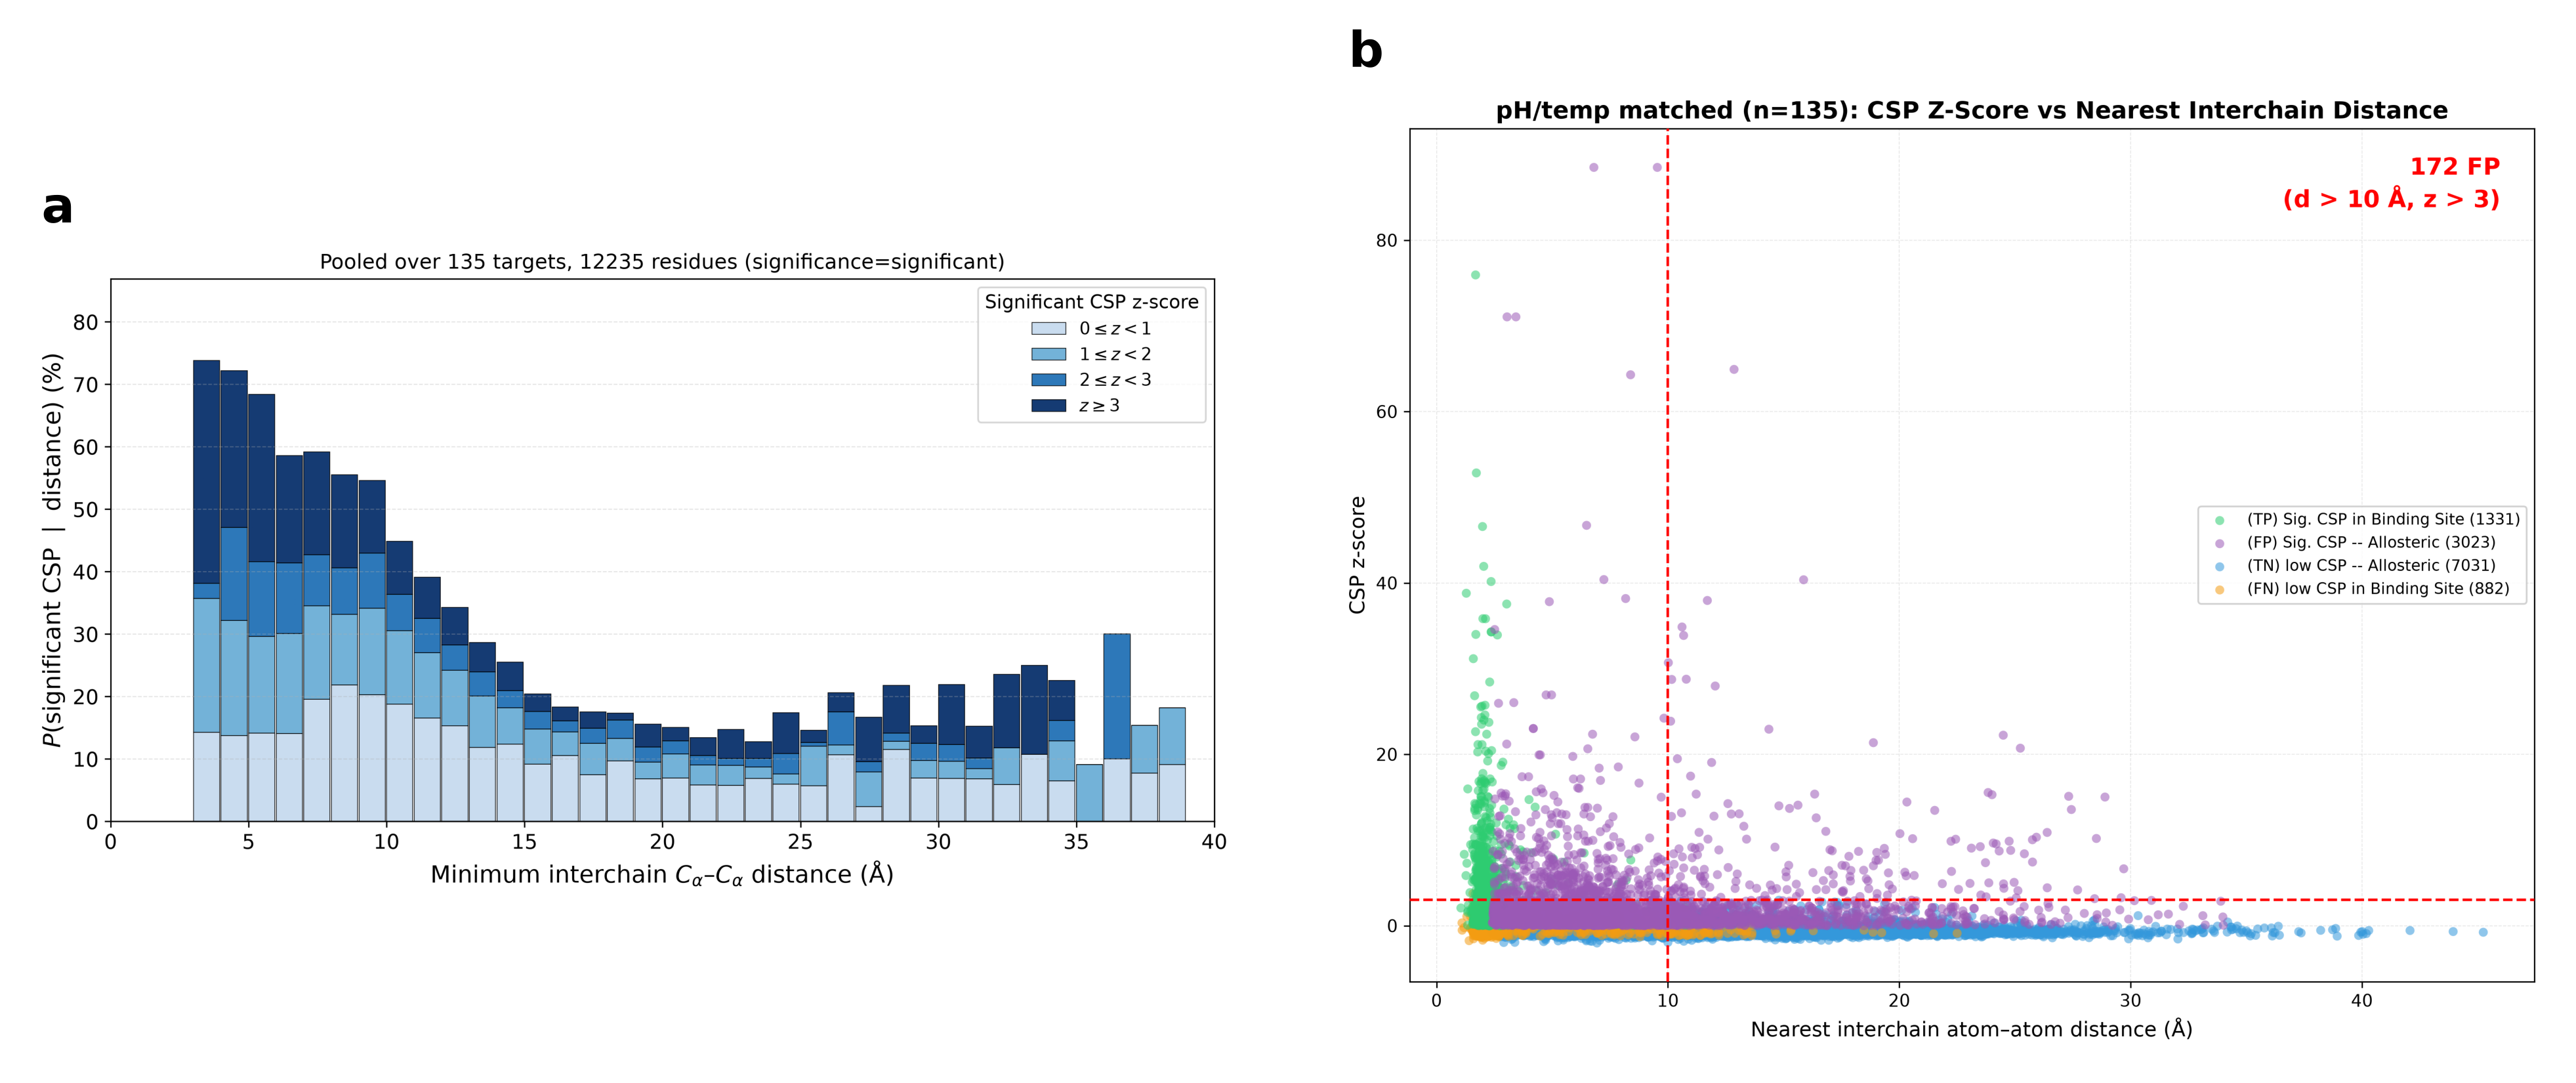
\includegraphics[width=\linewidth]{SF17_csp_vs_distance_panels.png}
\captionsetup{labelformat=empty}
\caption{\textbf{SI Fig. S17. Chemical-shift perturbations as a function of
interchain distance.}
\textbf{(a)} Residue-pooled
$P(\text{significant CSP}\mid\text{minimum interchain }C_\alpha\text{--}C_\alpha\text{ distance})$
for buffer-similar systems ($n=135$ from
\texttt{CSP\_UBQ\_ph0.5\_temp5C.csv} with pipeline outputs) under the primary cutoff
$\max(\text{cleaned mean},\,0.05\,\mathrm{ppm})$.
Bar height is the fraction of residues with a recorded HN CSP that are called
significant in each 1\,\AA{} distance bin; stacks partition those significant
CSPs by cleaned-mean $z$-score
($0\leq z<1$, $1\leq z<2$, $2\leq z<3$, $z\geq 3$).
Close to the interface the significant fraction is high and enriched in large
$z$, then declines toward a lower baseline at longer range.
\textbf{(b)} Per-residue CSP $z$-score versus nearest interchain any-atom
distance for the same $n=135$ set (same primary significance definition), colored by confusion-matrix
class (TP/FP/TN/FN) relative to the structural binding-site mask.
Dashed lines mark $z=3$ and $d=10$\,\AA{}; the annotation counts false positives
with $d>10$\,\AA{} and $z>3$.}
\end{figure}

\begin{figure}[H]
\centering
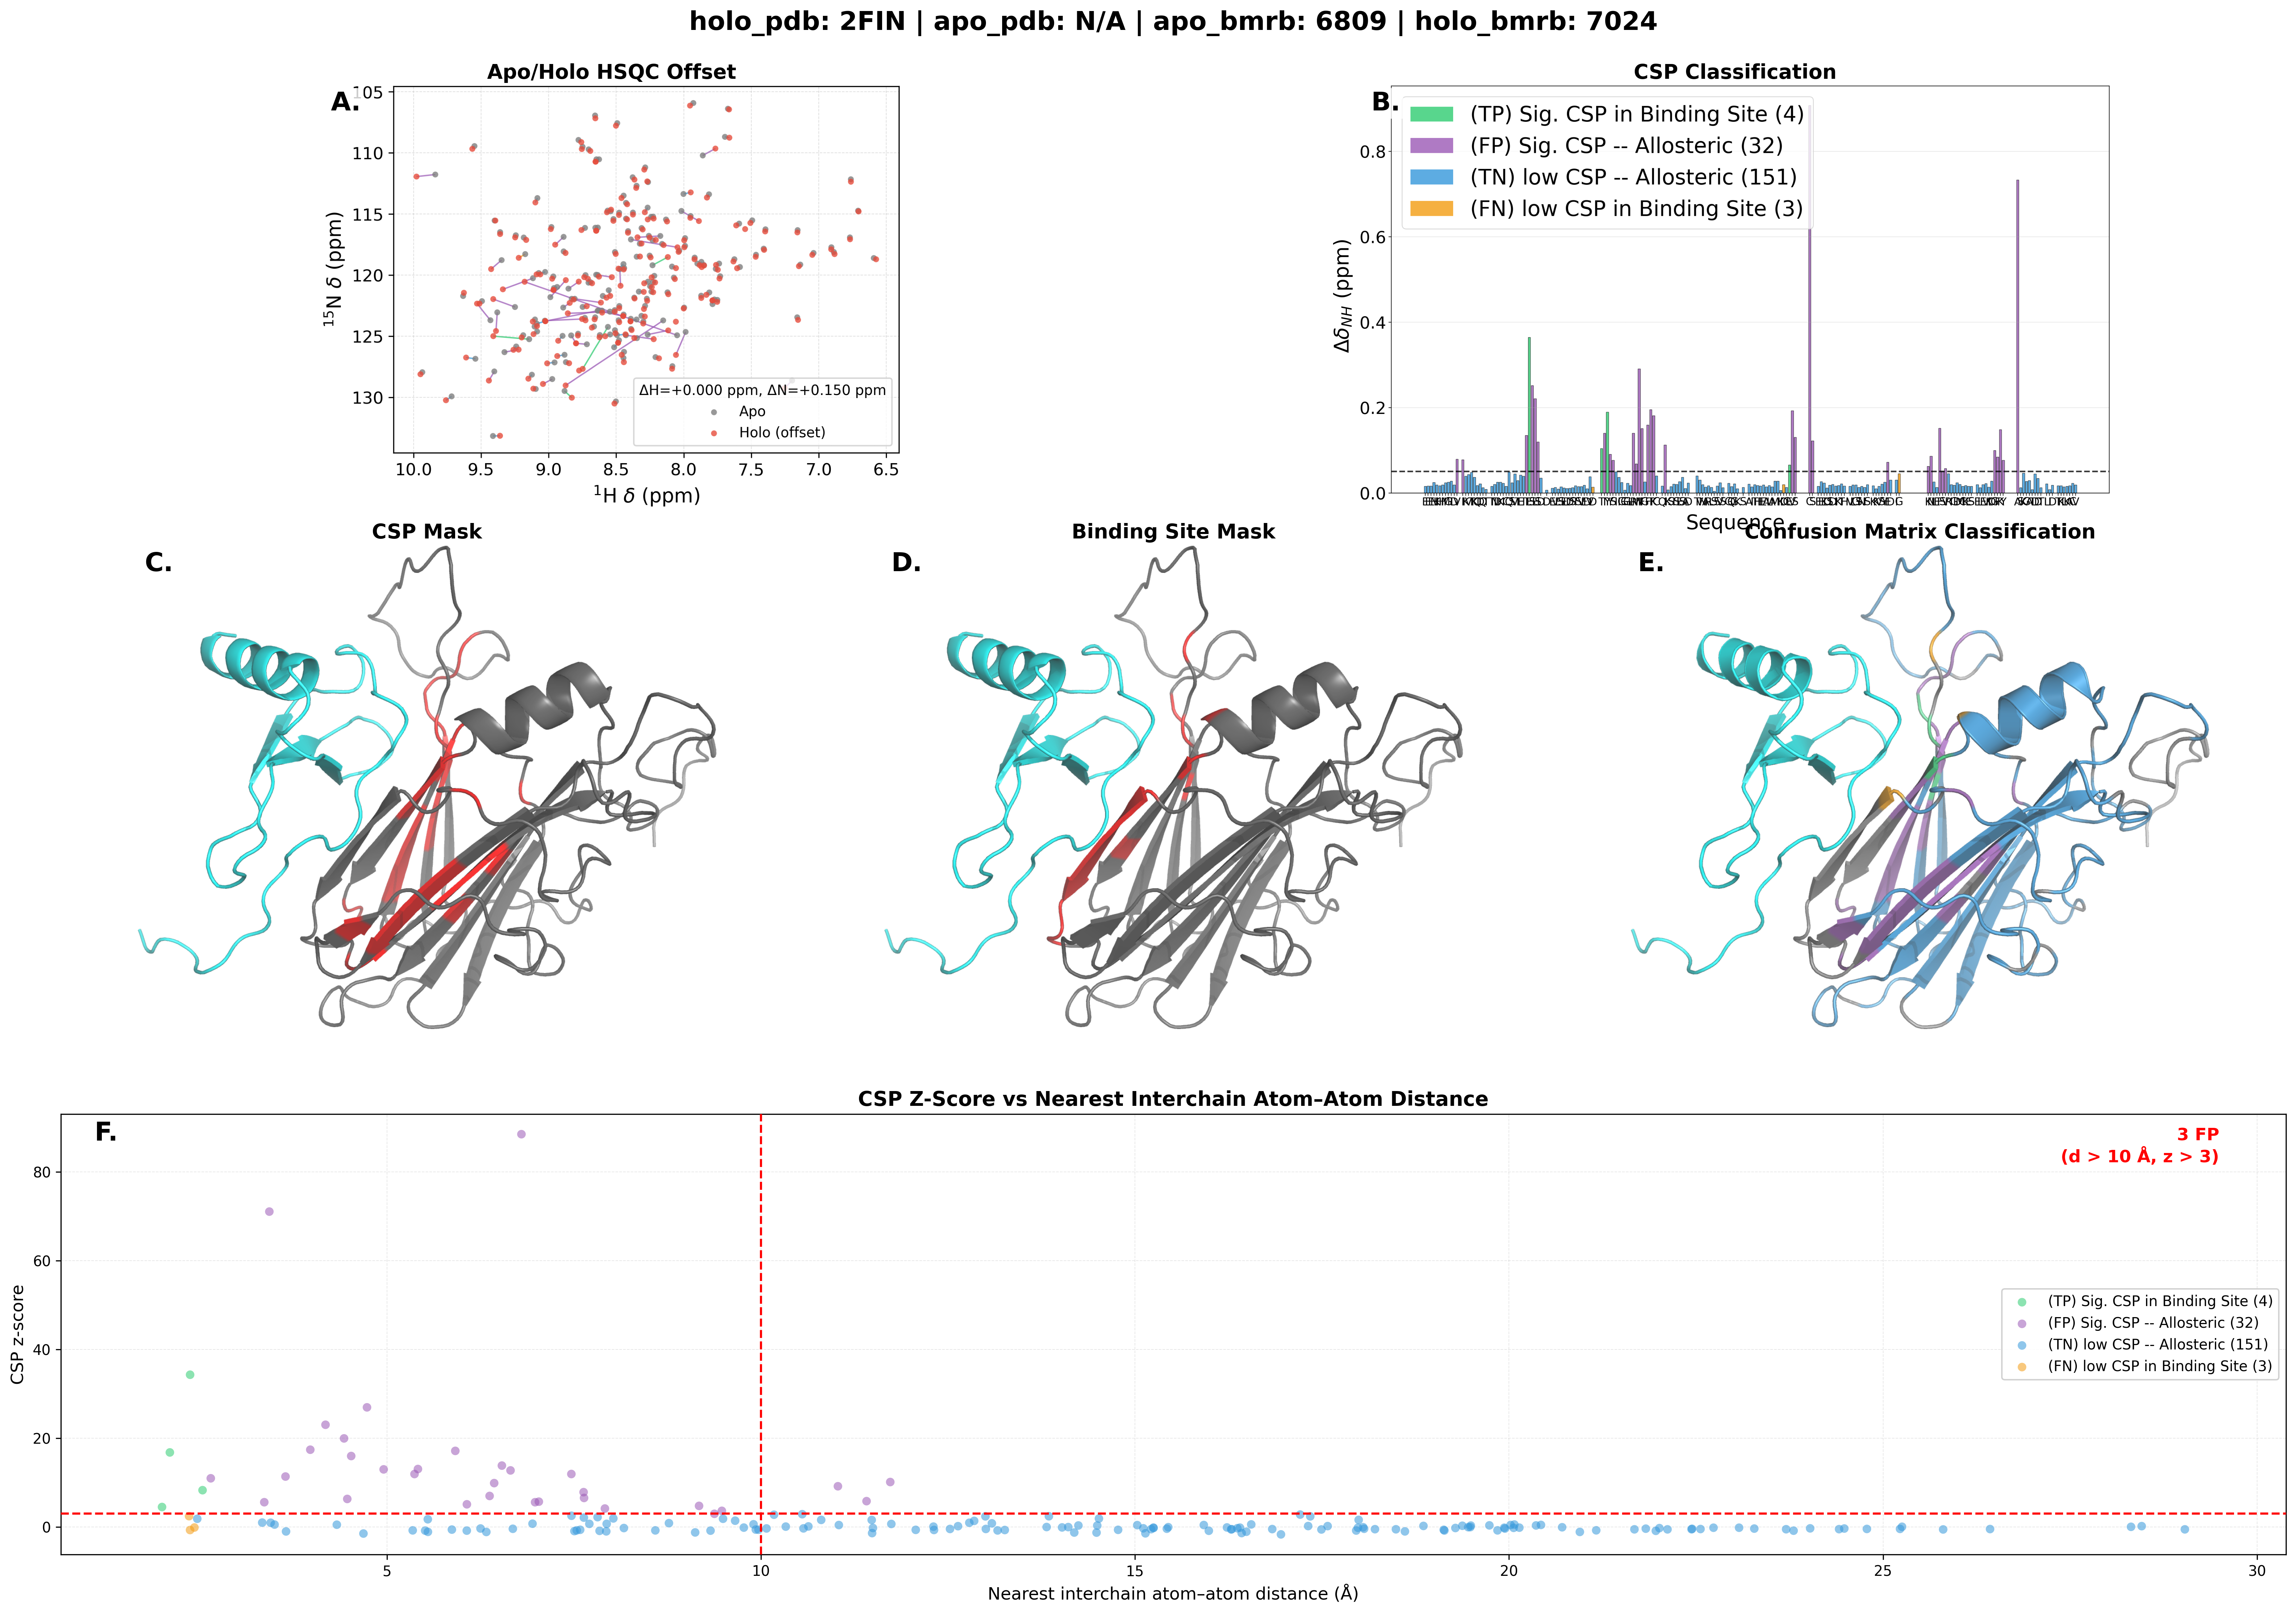
\includegraphics[width=\linewidth]{SF18_2FIN_case_study_z.png}
\captionsetup{labelformat=empty}
\caption{\textbf{SI Fig. S18. Case study for holo 2FIN / apo BMRB 6809}
(holo BMRB 7024).
HSQC overlay, CSP classification bars, CSP / binding-site / confusion structure
views, and CSP $z$ versus nearest interchain atom--atom distance.
\textbf{(F)} Dashed lines mark $z=3$ and $d=10$\,\AA{}; the annotation counts
false positives with $d>10$\,\AA{} and $z>3$.
This plot shows monotonic decay of CSPs with increasing nearest interchain
atom--atom distance.
Residues in a set of $\beta$ sheets further away from the ligand with
significant shifts have lower CSPs than those closer to the binding site.}
\end{figure}

% SF19 is a static PDB Advanced Search screenshot (no generator).
\IfFileExists{../../figures/SF19_pdb_search.png}{%
\begin{figure}[H]
\centering
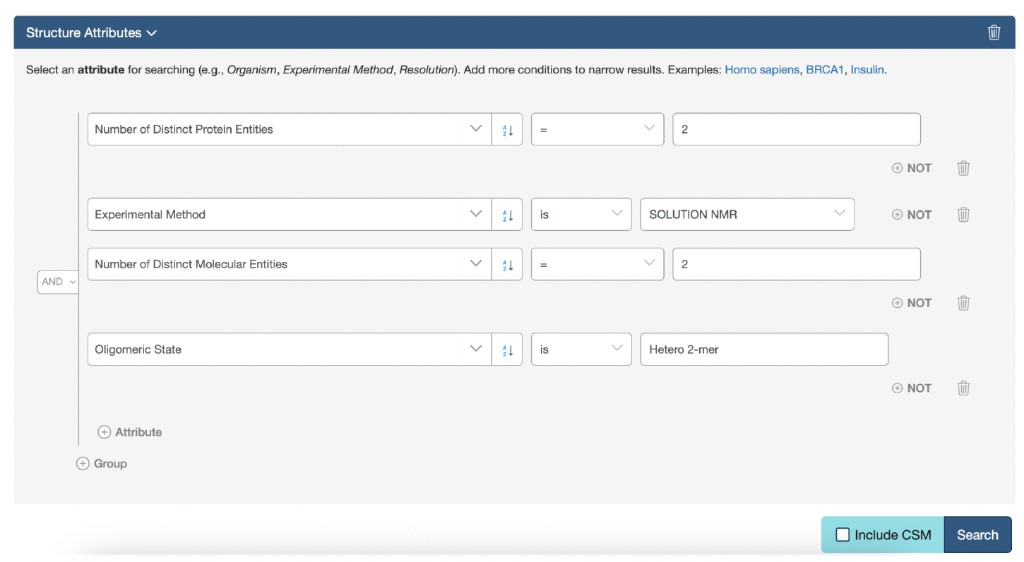
\includegraphics[width=\linewidth]{SF19_pdb_search.png}
\captionsetup{labelformat=empty}
\caption{\textbf{SI Fig. S19. PDB Advanced Search Settings.}
For the subset of targets manually scraped from the PDB, we restrict our
analysis to these settings: entries resolved by Solution NMR, with two and
only two distinct protein chains. At the time of curation, this advanced
search resulted in 720 hits on the RCSB PDB. From this list of 720, entries
were included in the CSP DB if there were N and H chemical shifts deposited
in the BMRB for an identical sequence which was evaluated in both apo and
holo experiments.}
\end{figure}
\clearpage
}{}

\begin{figure}[H]
\centering
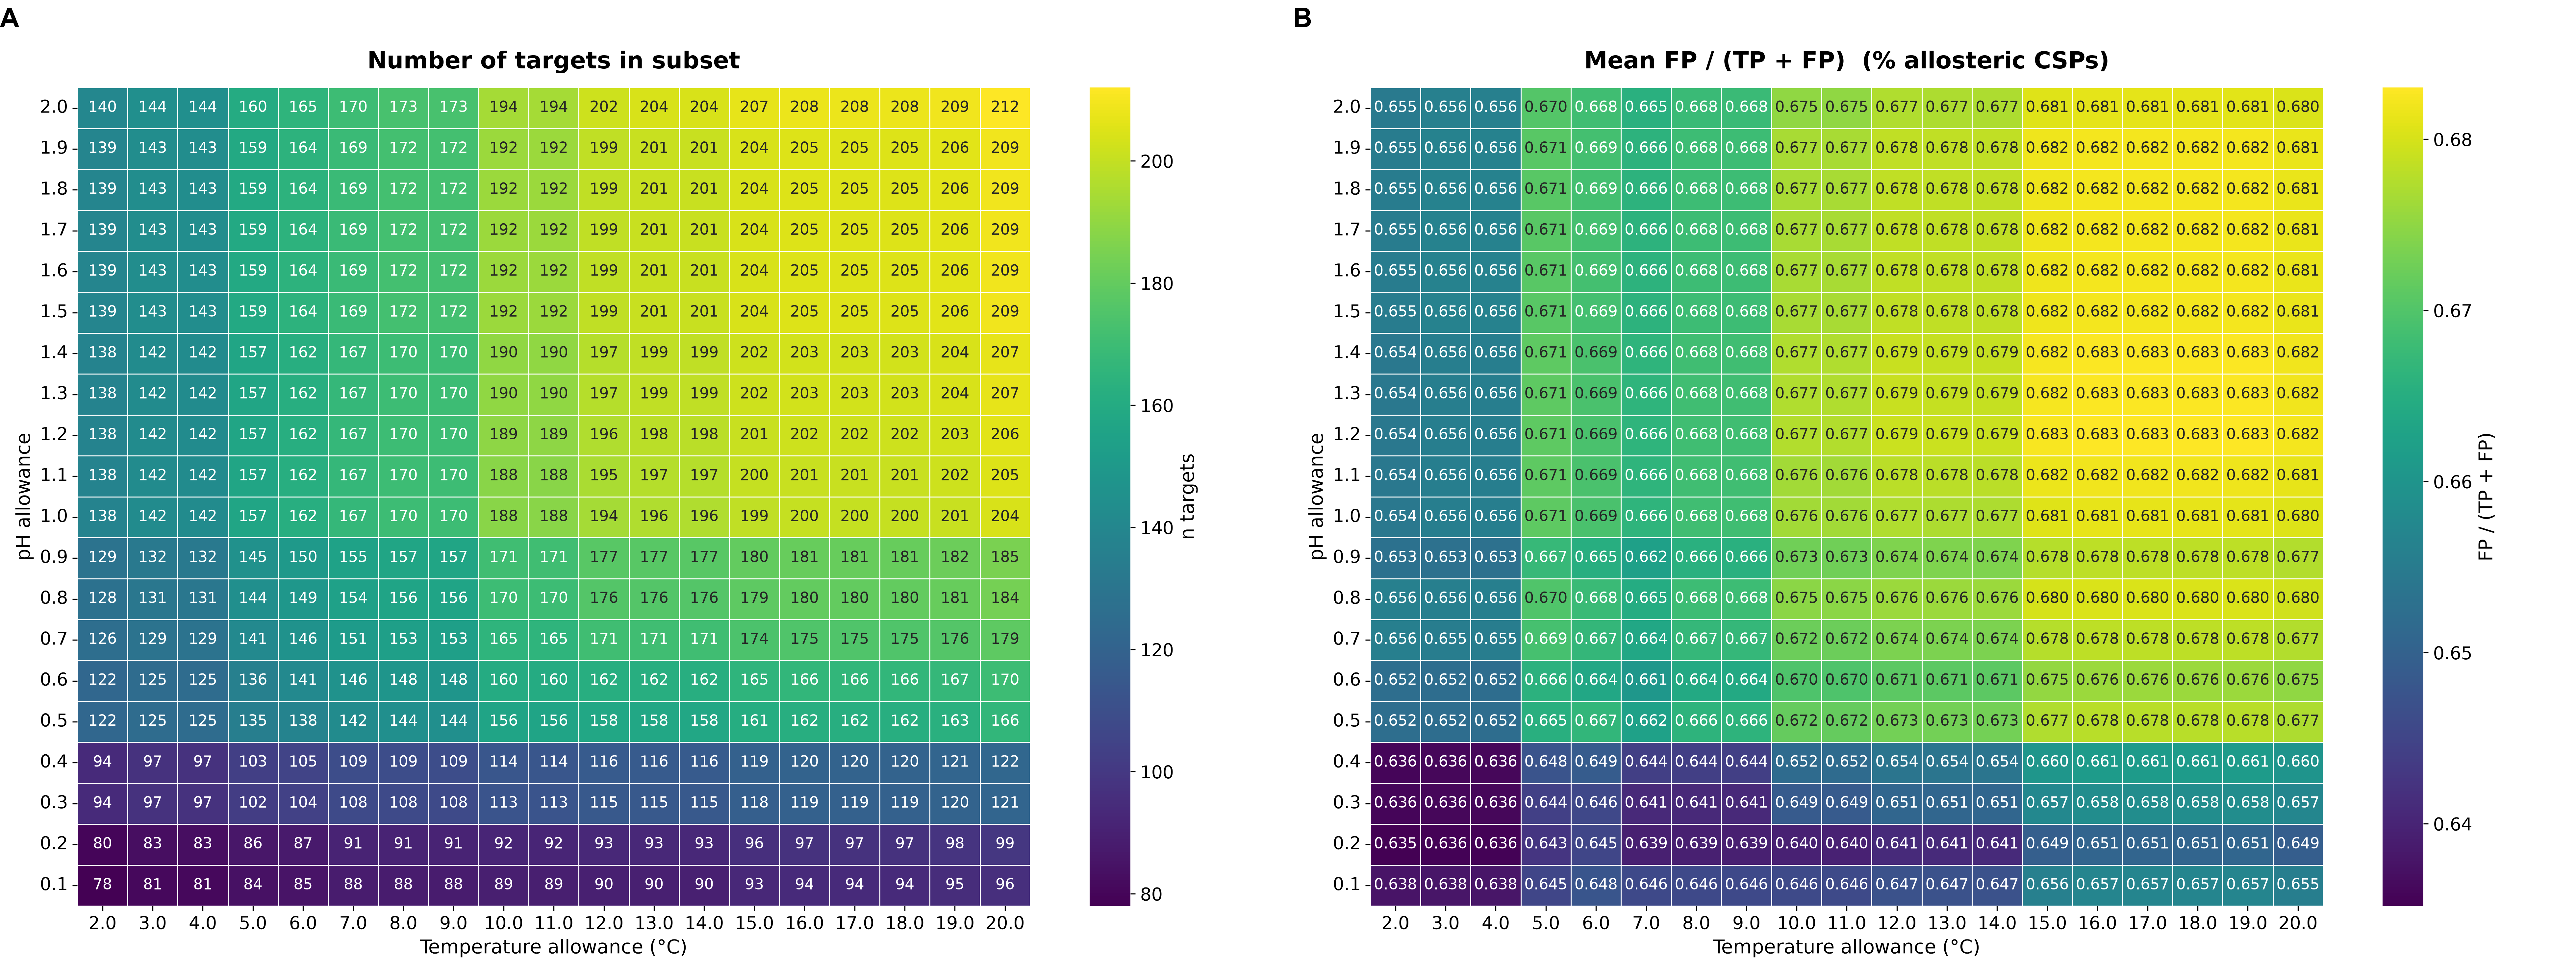
\includegraphics[width=\linewidth]{SF20_buffer_sweep.png}
\captionsetup{labelformat=empty}
\caption{\textbf{SI Fig. S20. Buffer pH/temperature threshold sweep.}
(\textbf{A}) Number of apo/holo pairs retained as $|\Delta\mathrm{pH}|$ and
$|\Delta T|$ thresholds are tightened.
(\textbf{B}) Mean FP/(TP+FP) (percent allosteric CSPs) in the same subsets.}
\end{figure}

\begin{figure}[H]
\centering
\textbf{(A)}\\[0.15em]
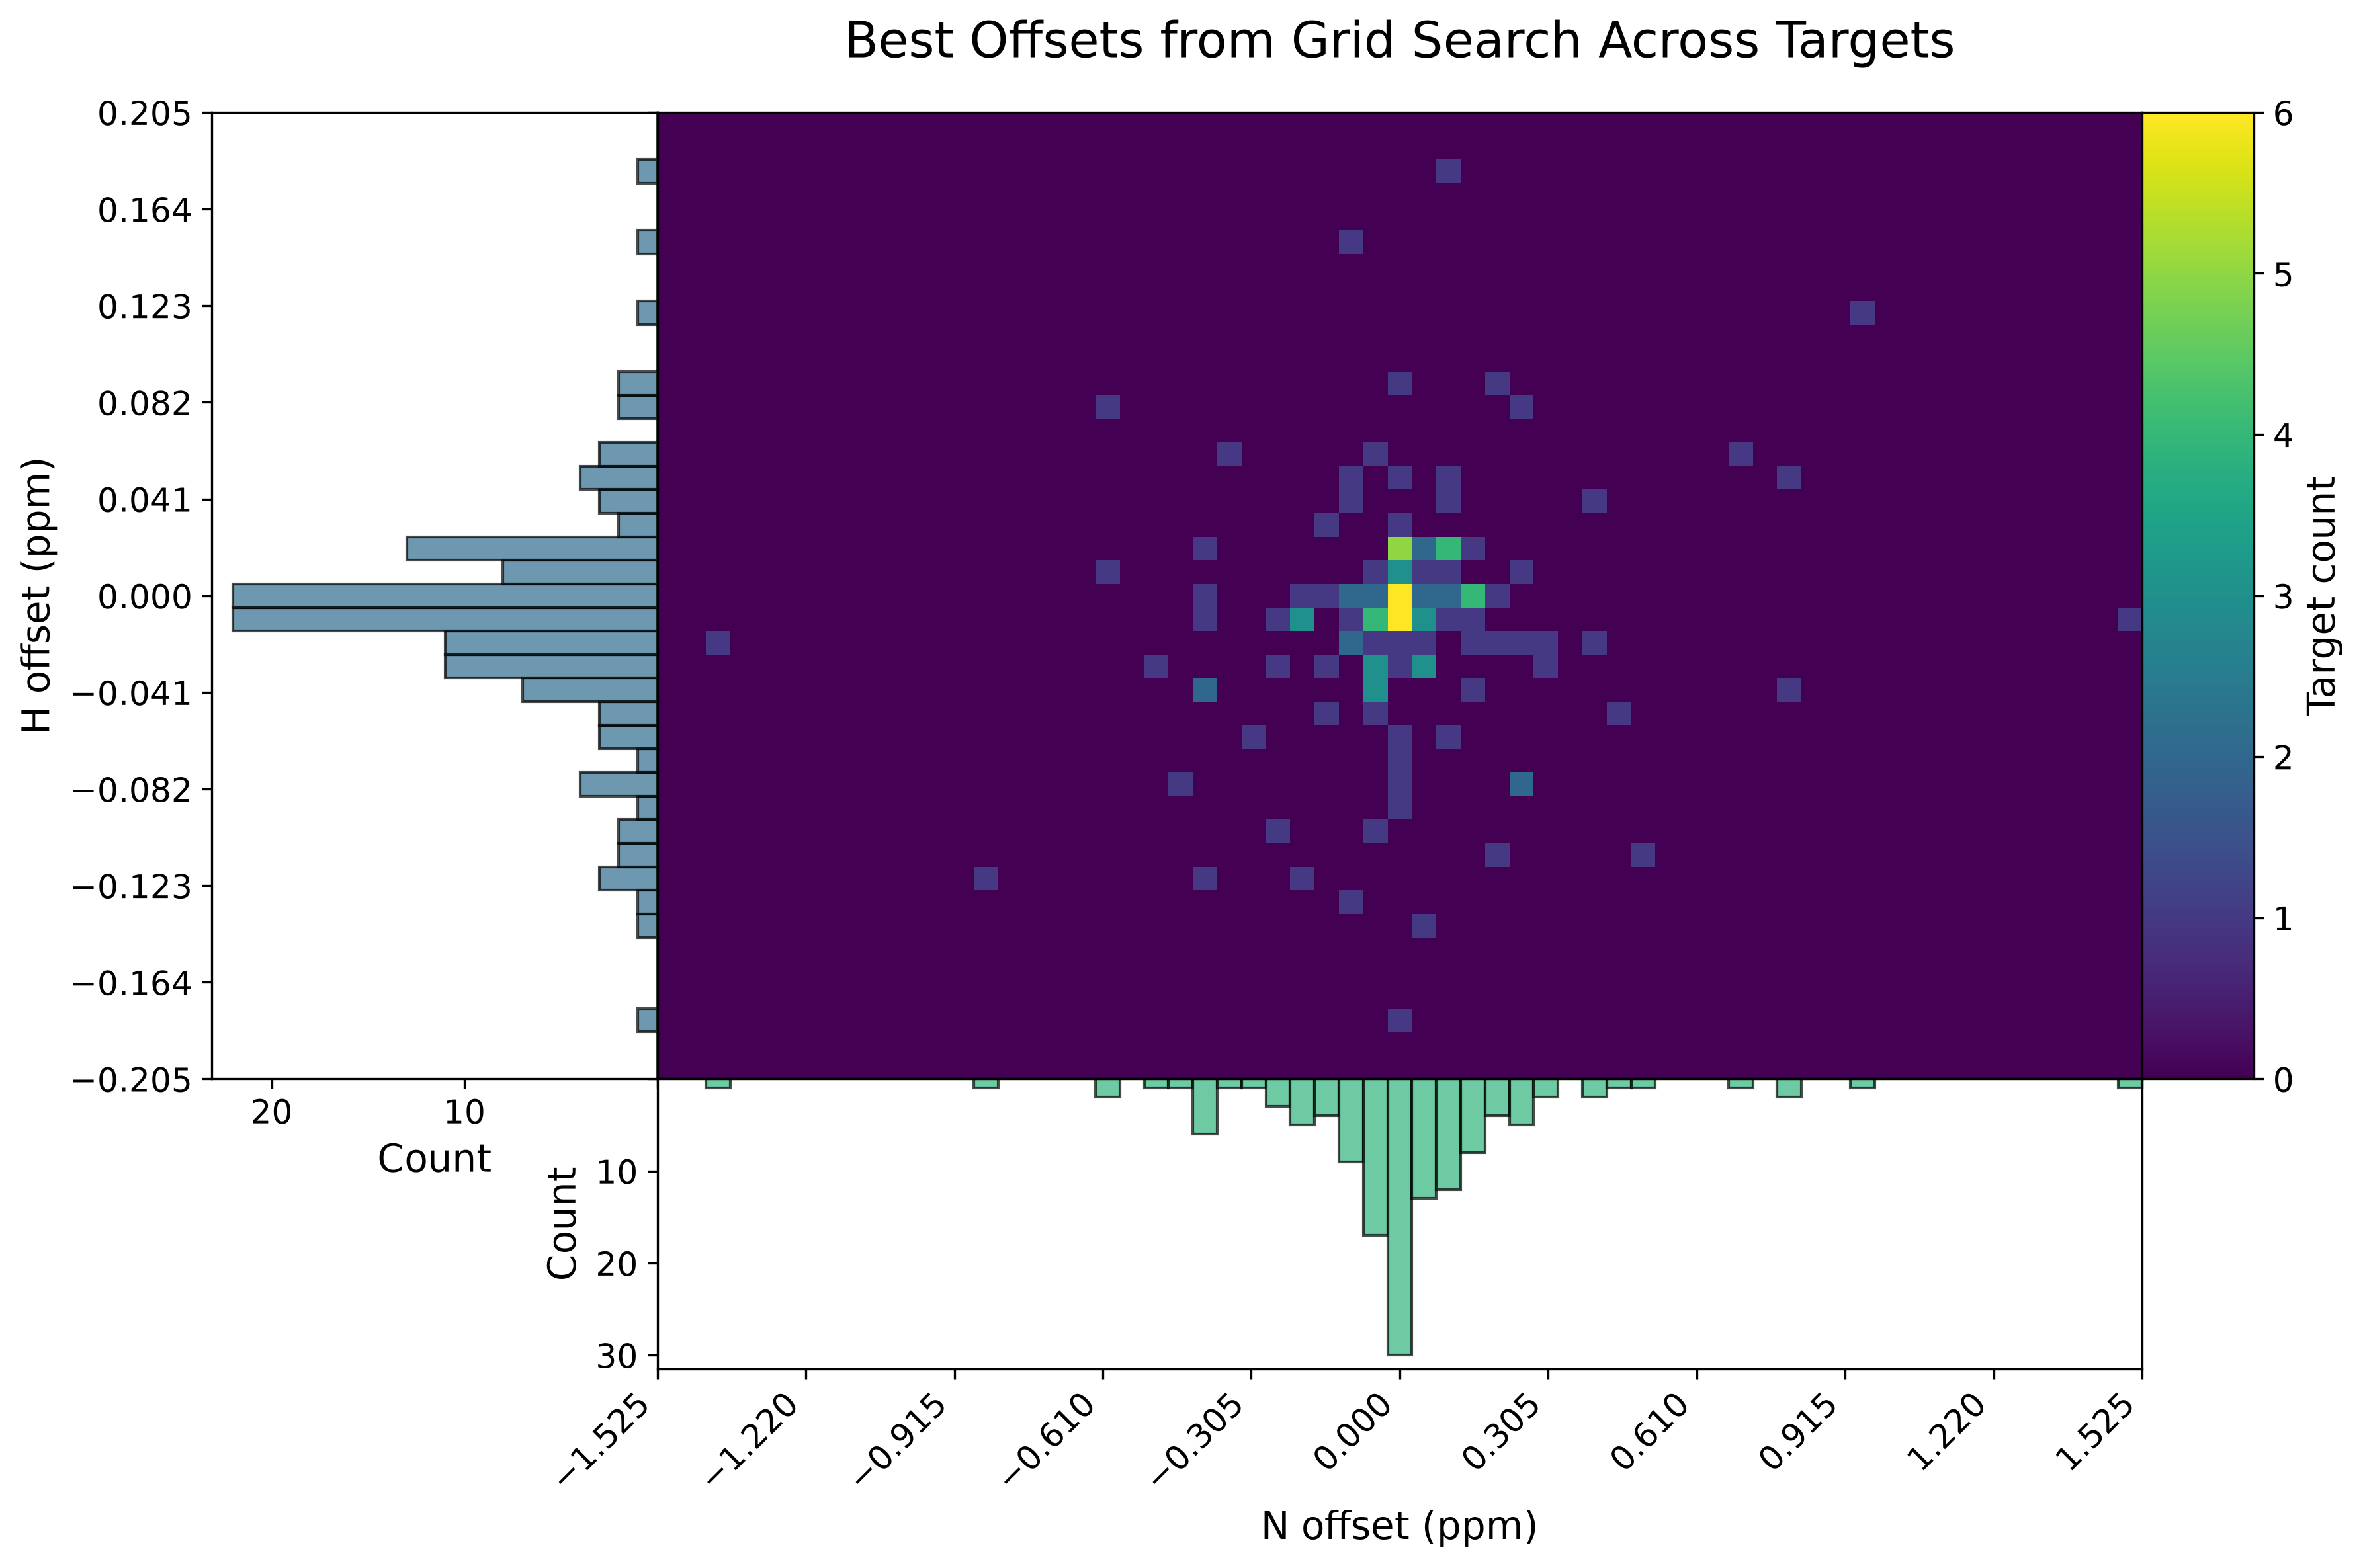
\includegraphics[width=0.78\linewidth]{SF21_ideal_offsets.png}\\[0.4em]
\textbf{(B)}\\[0.15em]
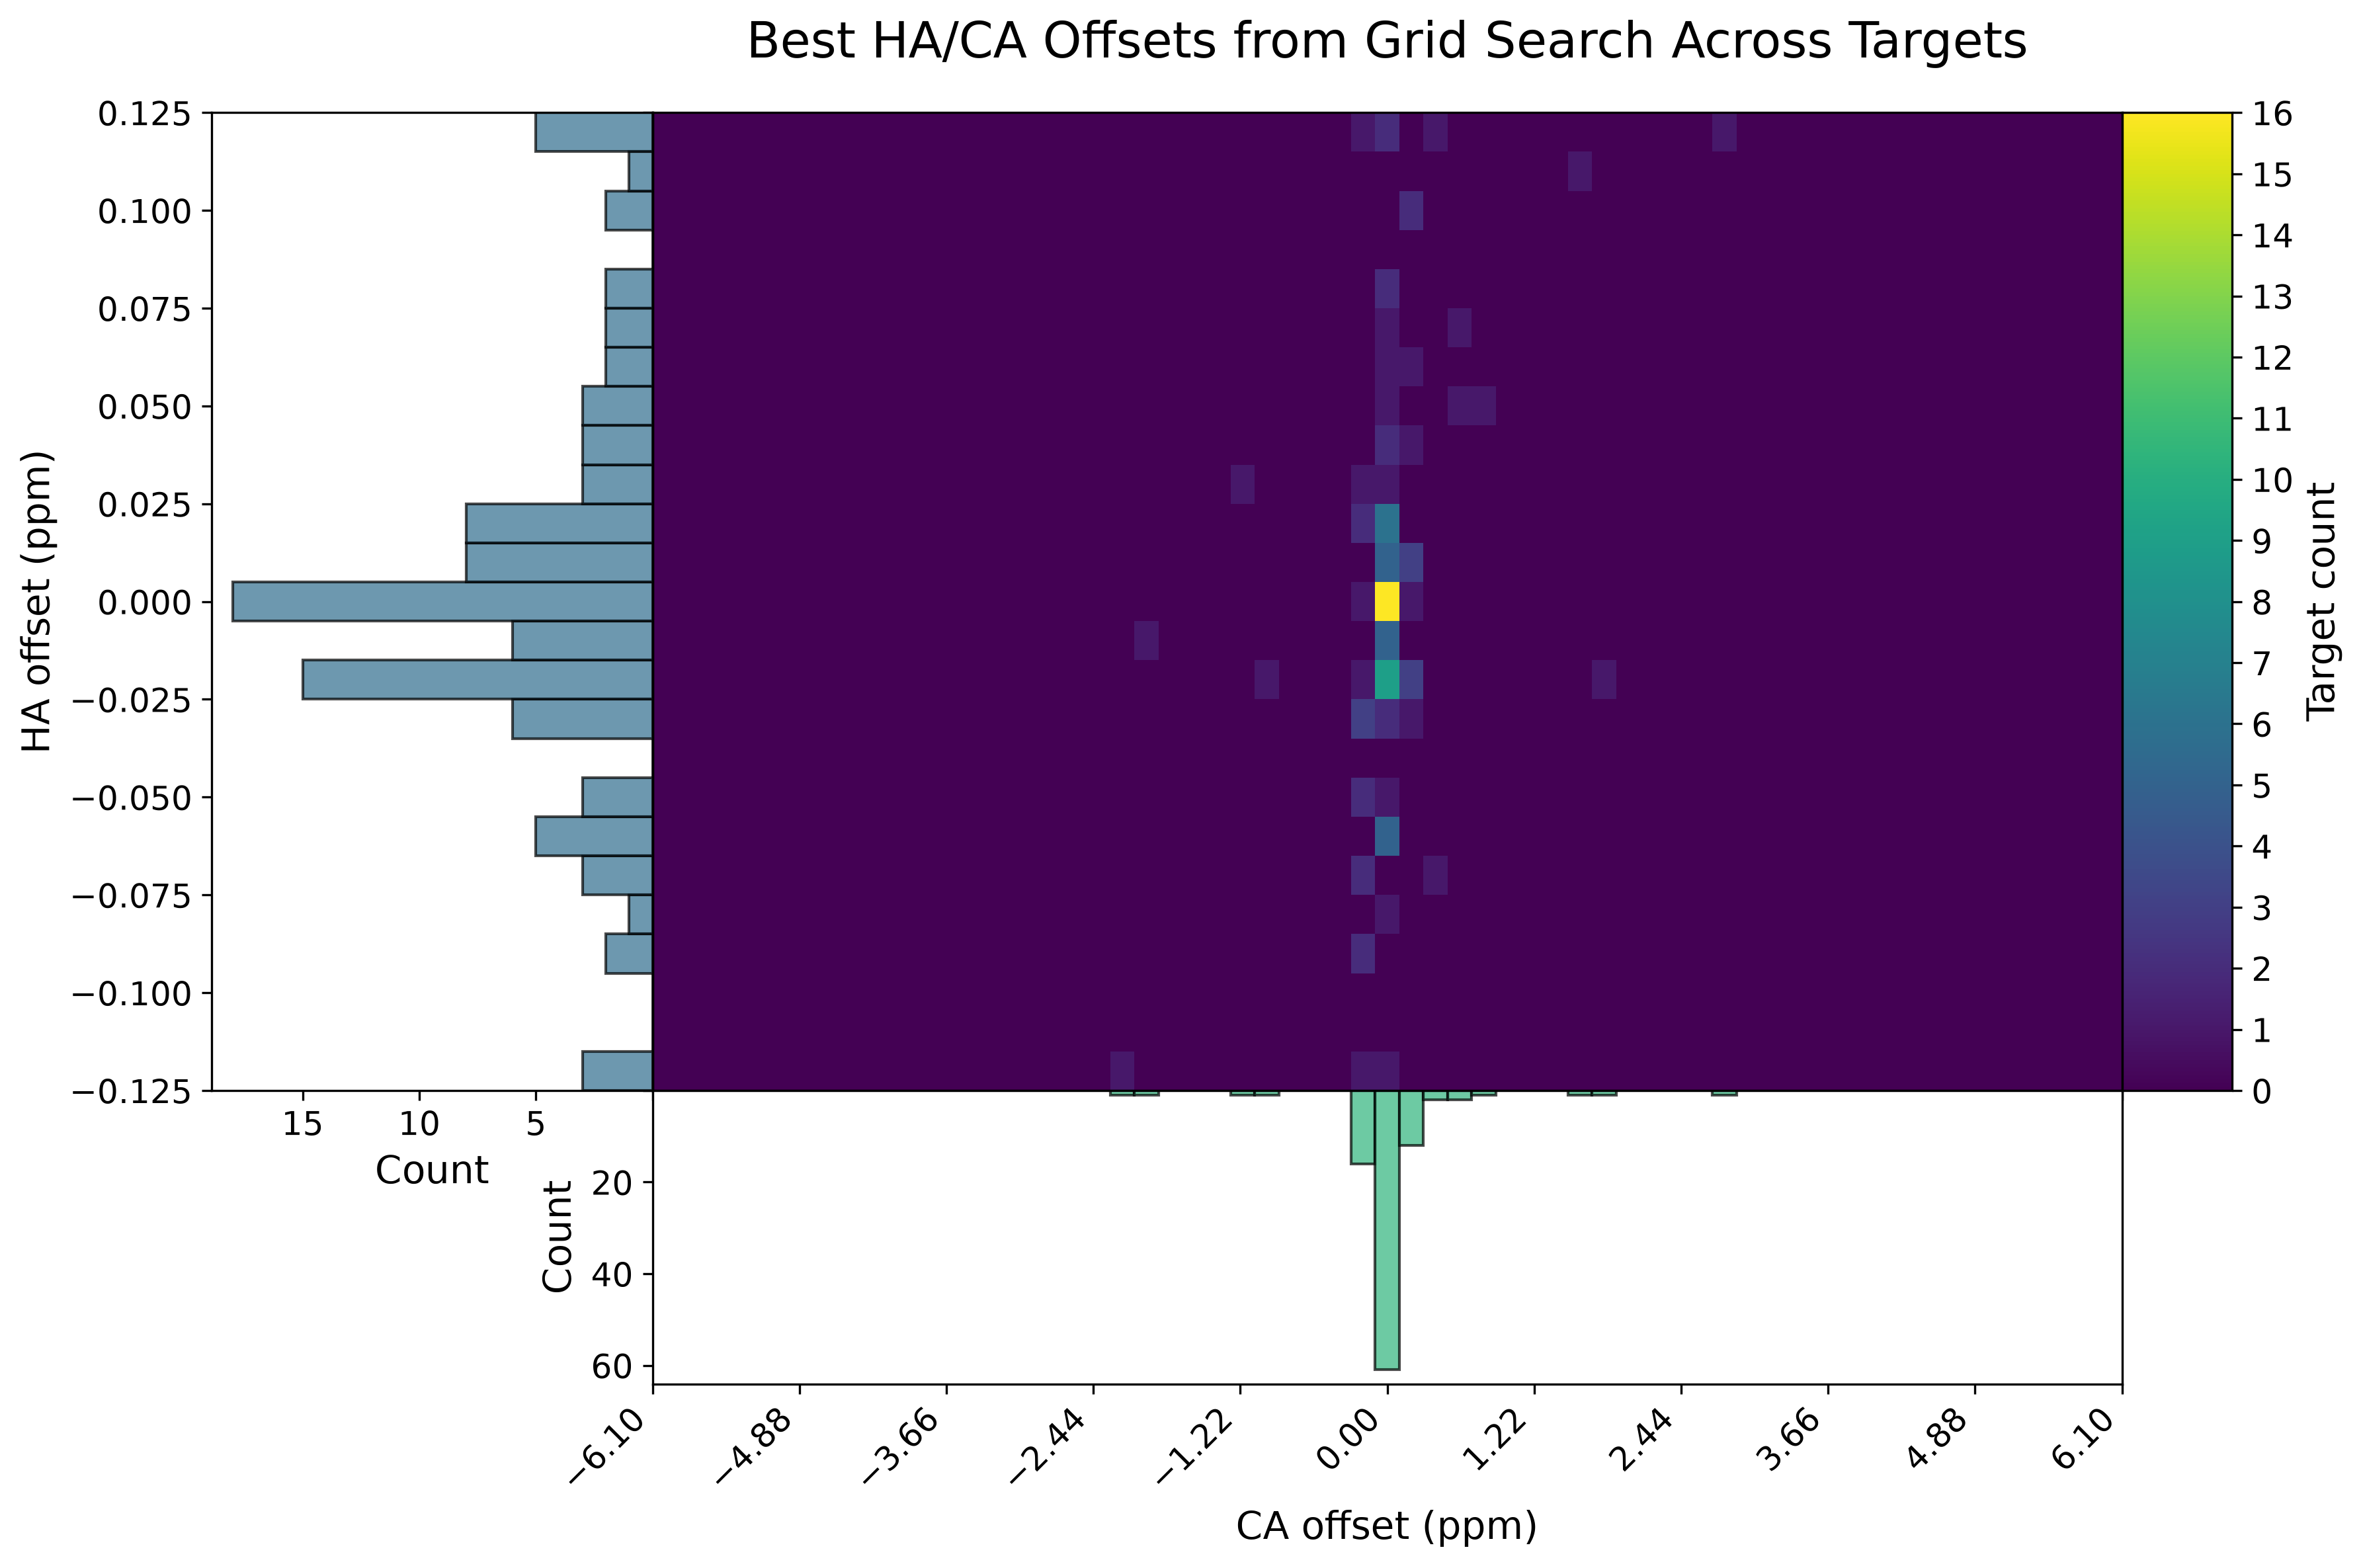
\includegraphics[width=0.78\linewidth]{SF21_ideal_offsets_ha_ca.png}
\captionsetup{labelformat=empty}
\caption{\textbf{SI Fig. S21. Ideal chemical-shift offset grids}
for buffer-similar systems in \texttt{CSP\_UBQ\_ph0.5\_temp5C.csv} with
pipeline outputs.
(\textbf{A}) H/N referencing ($n=135$): a grid search selects the H/N offsets
that maximize aligned HN peak counts under the pipeline CSP criterion; the
heatmap aggregates those optimal
$(\Delta\delta_{\mathrm{N}},\,\Delta\delta_{\mathrm{H}})$ pairs
(color $=$ number of targets).
Marginal histograms show the one-dimensional distributions of best H (left) and
N (bottom) offsets.
(\textbf{B}) HA/CA referencing ($n=101$ systems with HA/CA grid-search CSVs):
the same layout for offsets that maximize aligned HA/CA peak counts,
with HA (left) and CA (bottom) marginals.
Both nuclei pairs are peaked near zero, indicating that most apo/holo pairs
require only small referencing corrections.}
\end{figure}

\begin{figure}[H]
\centering
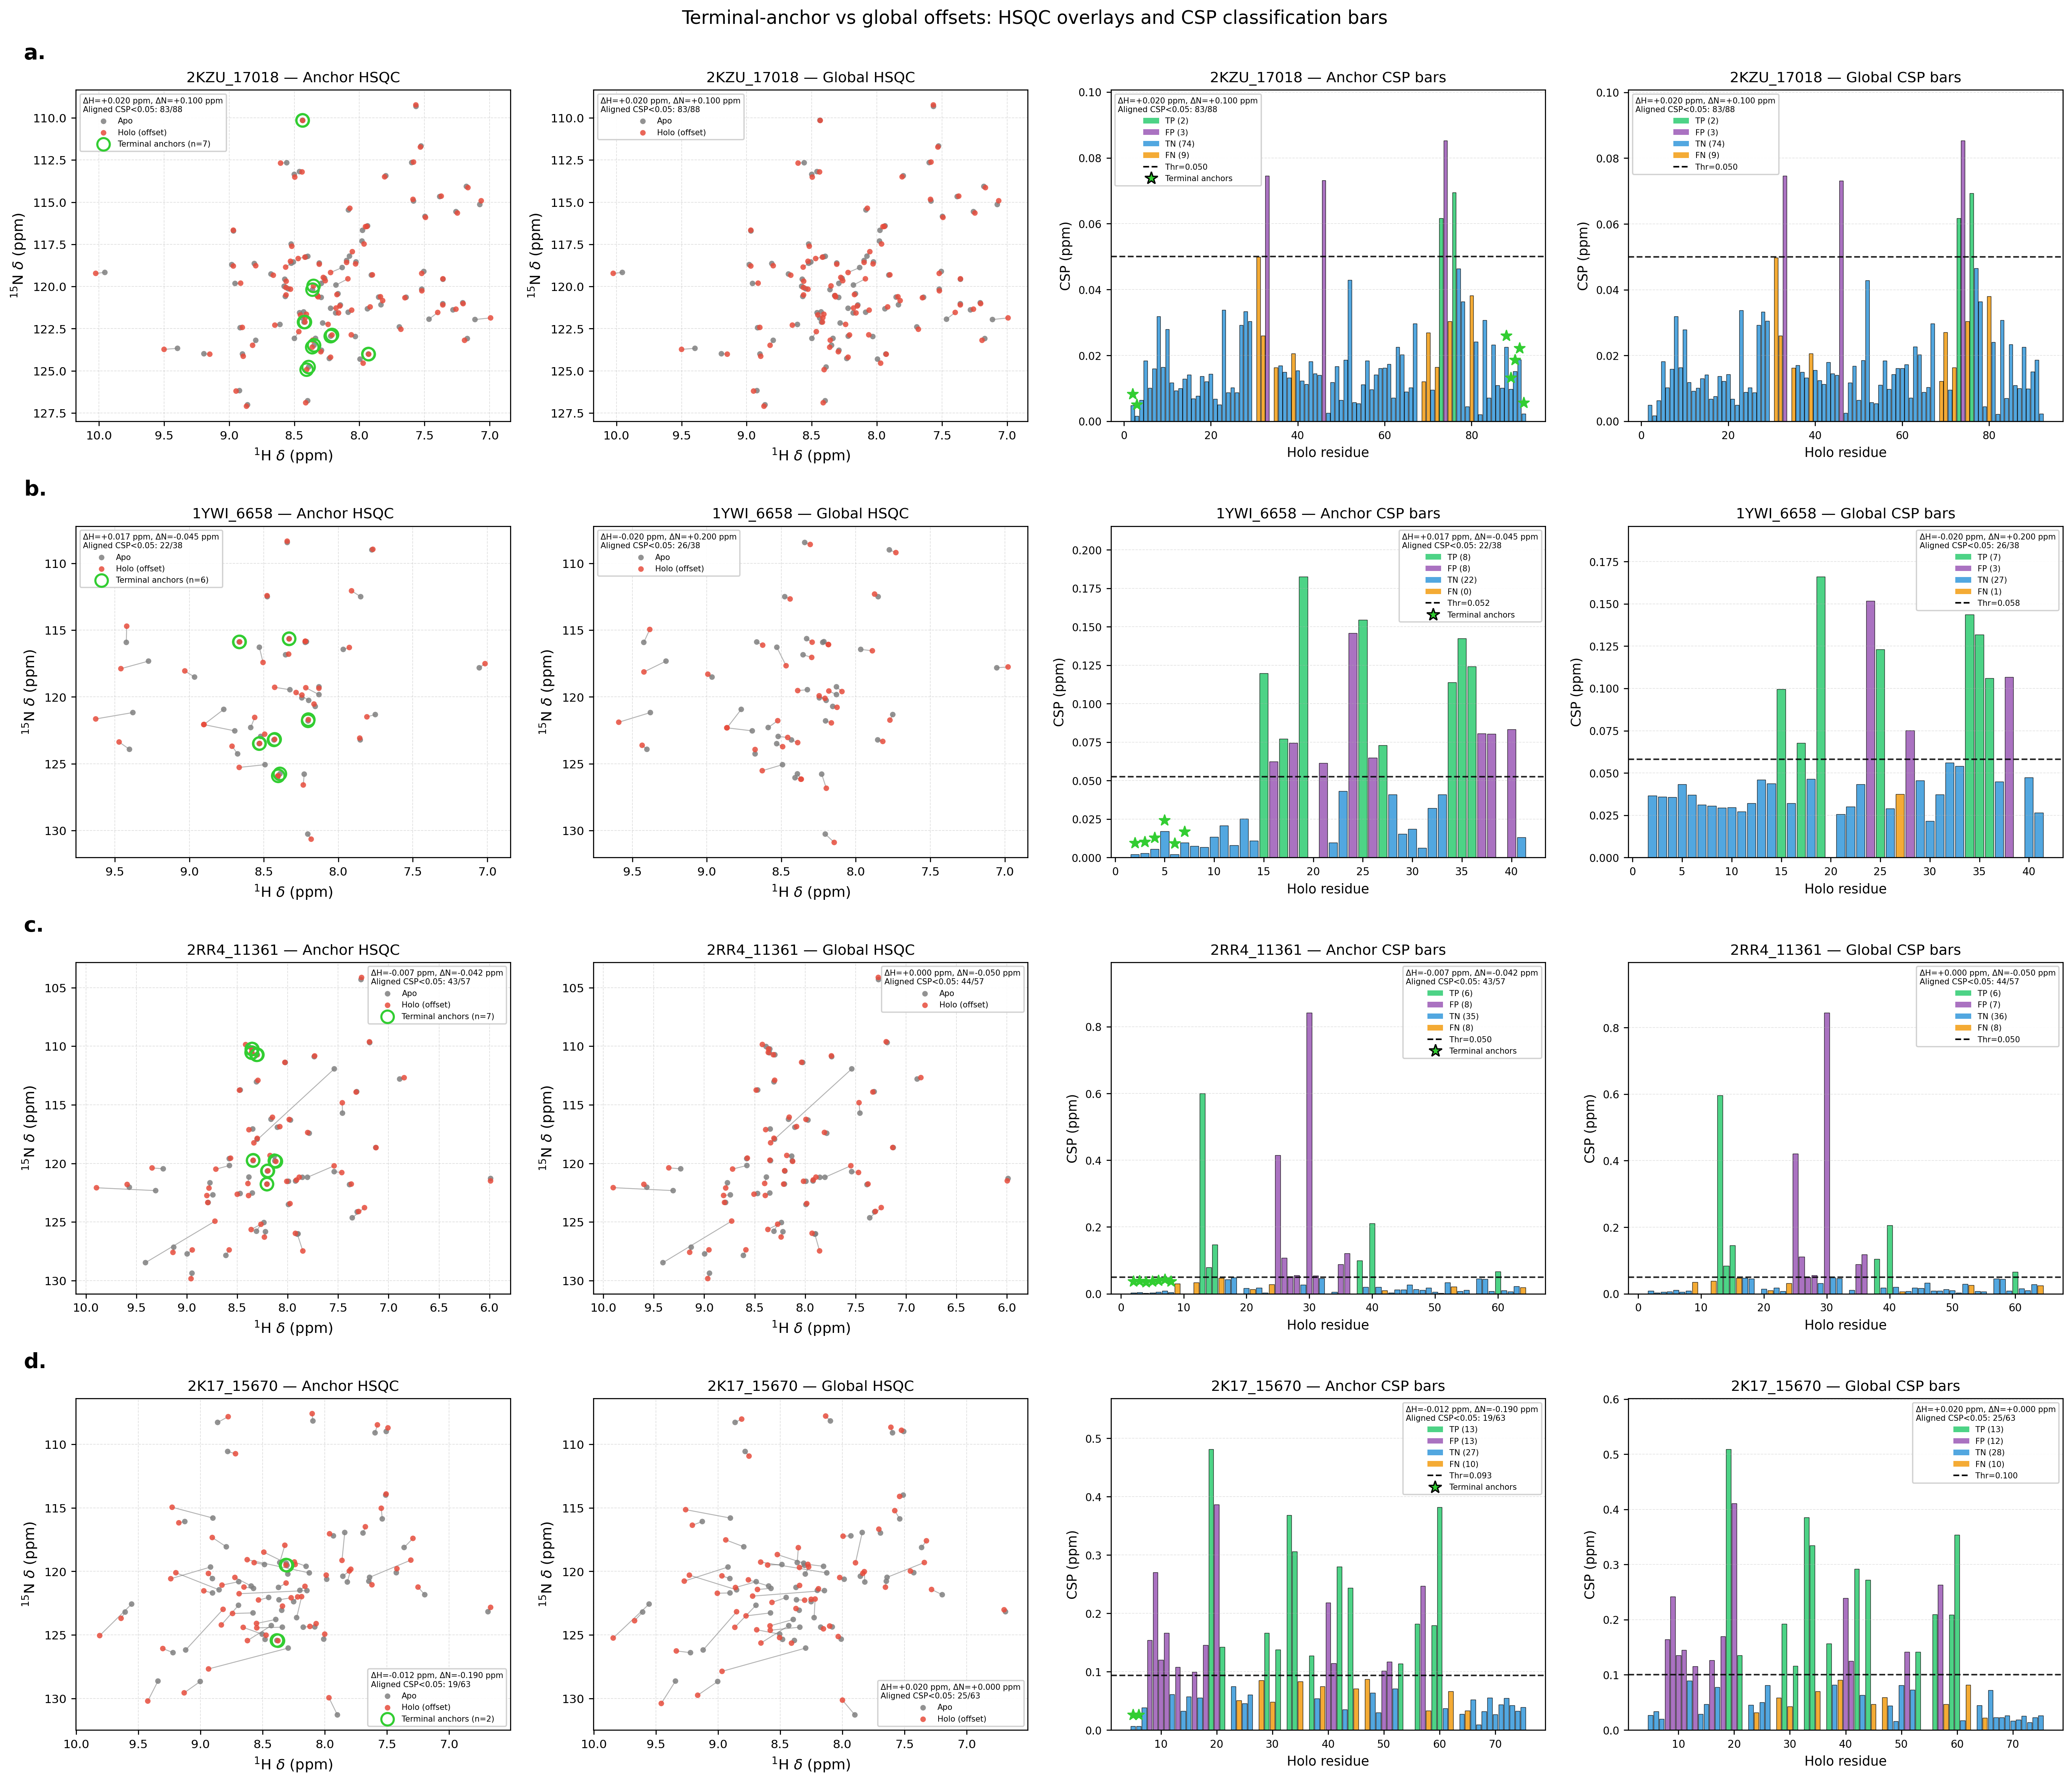
\includegraphics[width=\linewidth]{SF22_terminal_anchor_vs_global.png}
\captionsetup{labelformat=empty}
\caption{\textbf{SI Fig. S22. Terminal-anchor vs global offsets:}
HSQC overlays and CSP classification bars for four targets
(2KZU/17018, 1YWI/6658, 2RR4/11361, 2K17/15670).
For each target (rows a--d): left pair shows apo (grey) vs offset holo (red)
HSQC overlays using terminal-anchor RMSD offsets vs the global CSP-count grid;
right pair shows corresponding CSP classification bars (TP/FP/TN/FN) under the
primary significance threshold. Green markers denote terminal-anchor residues.}
\end{figure}

\begin{figure}[H]
\centering
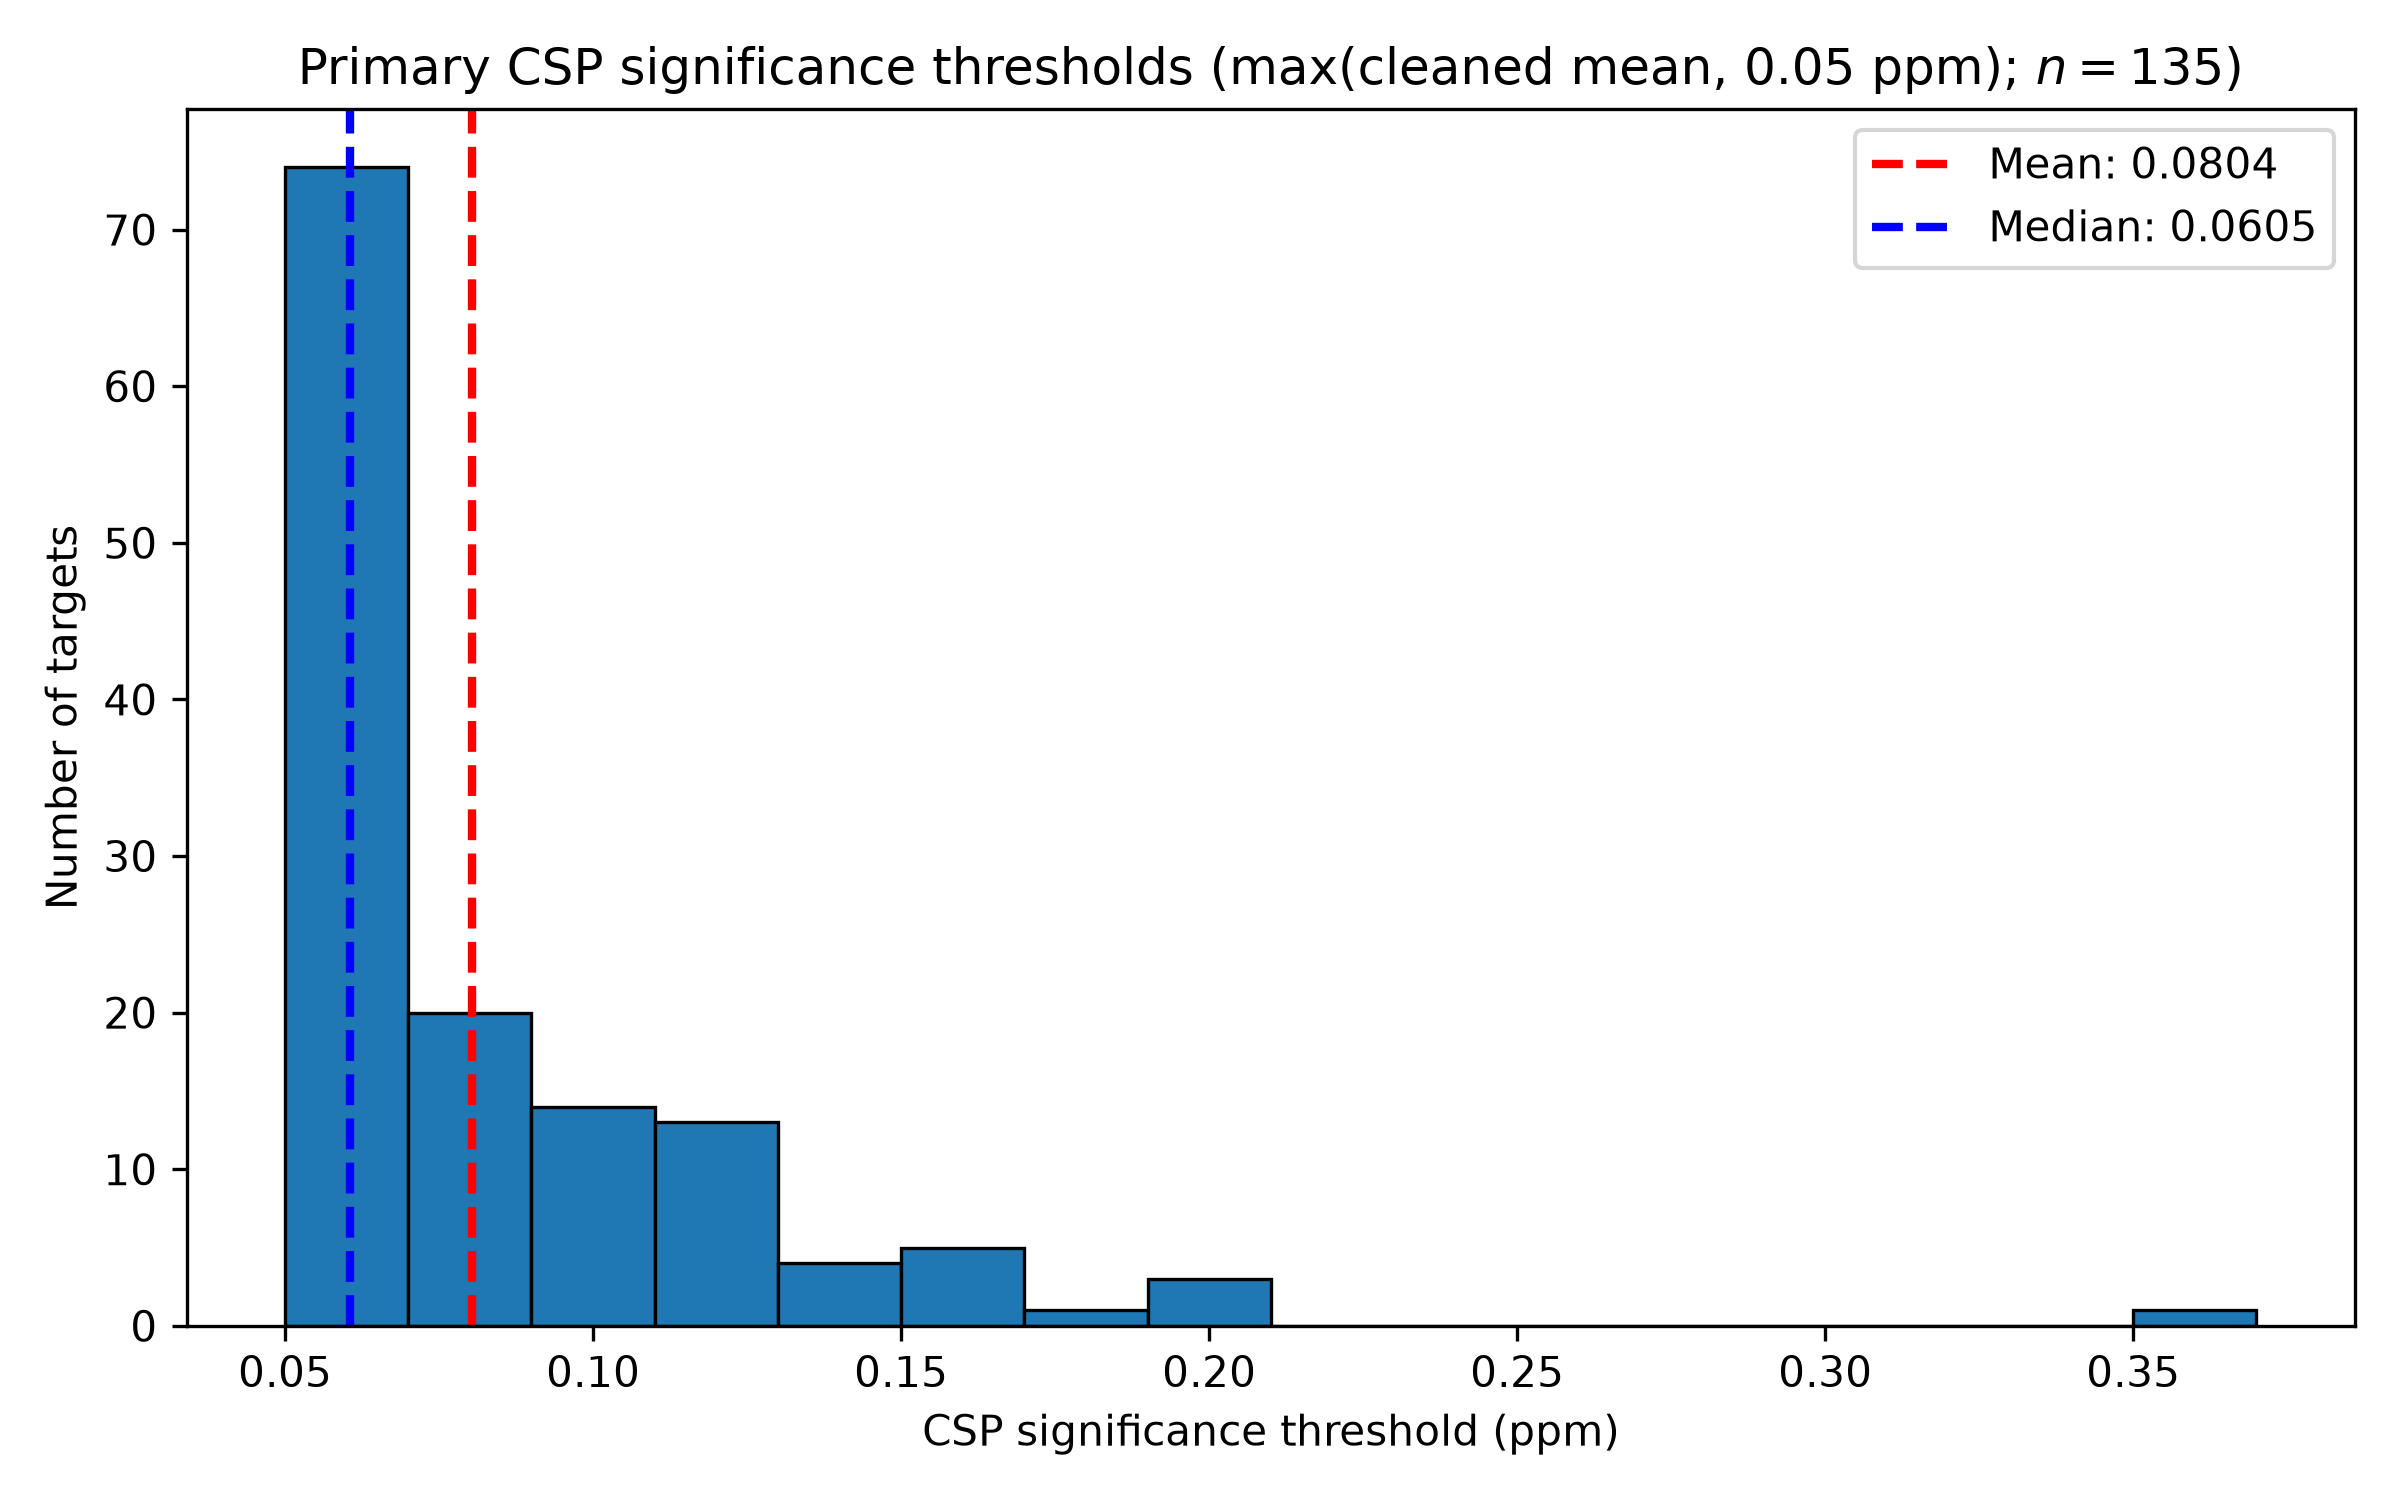
\includegraphics[width=0.9\linewidth]{SF23_significance_threshold.png}
\captionsetup{labelformat=empty}
\caption{\textbf{SI Fig. S23. Distribution of CSP significance thresholds}
(primary cutoff $\max(\mathrm{cleaned\ mean},\,0.05\,\mathrm{ppm})$;
$n=135$ buffer-similar systems from \texttt{CSP\_UBQ\_ph0.5\_temp5C.csv}
with pipeline outputs). Mean $=0.0804$ ppm.}
\end{figure}

\begin{figure}[H]
\centering
\includegraphics[width=\linewidth]{SF24_figure_3_thresholds.png}
\captionsetup{labelformat=empty}
\caption{\textbf{SI Fig. S24. Figure~3-style CA-distance histograms under alternate HN CSP
significance thresholds} ($n=135$ buffer-similar systems from
\texttt{CSP\_UBQ\_ph0.5\_temp5C.csv} with pipeline outputs).
Each column is a 3a (TP/FP among significant CSPs) $|$ 3b (full confusion) pair.
Thresholds (left to right, then continuing as labeled on the figure):
\textbf{primary} $\max(\text{cleaned mean},\,0.05\,\mathrm{ppm})$ after iterative
outlier removal;
\textbf{cleaned mean $+1$ SD} and \textbf{$+2$ SD};
\textbf{top 10\%} and \textbf{top 5\%} of HN CSP values;
fixed cutoffs \textbf{0.03}, \textbf{0.05}, and \textbf{0.10\,ppm};
\textbf{raw mean}, \textbf{raw mean $+1$ SD}, and \textbf{raw mean $+2$ SD}
(no outlier removal);
and \textbf{cleaned mean} without the 0.05\,ppm floor.}
\end{figure}

\begin{figure}[H]
\centering
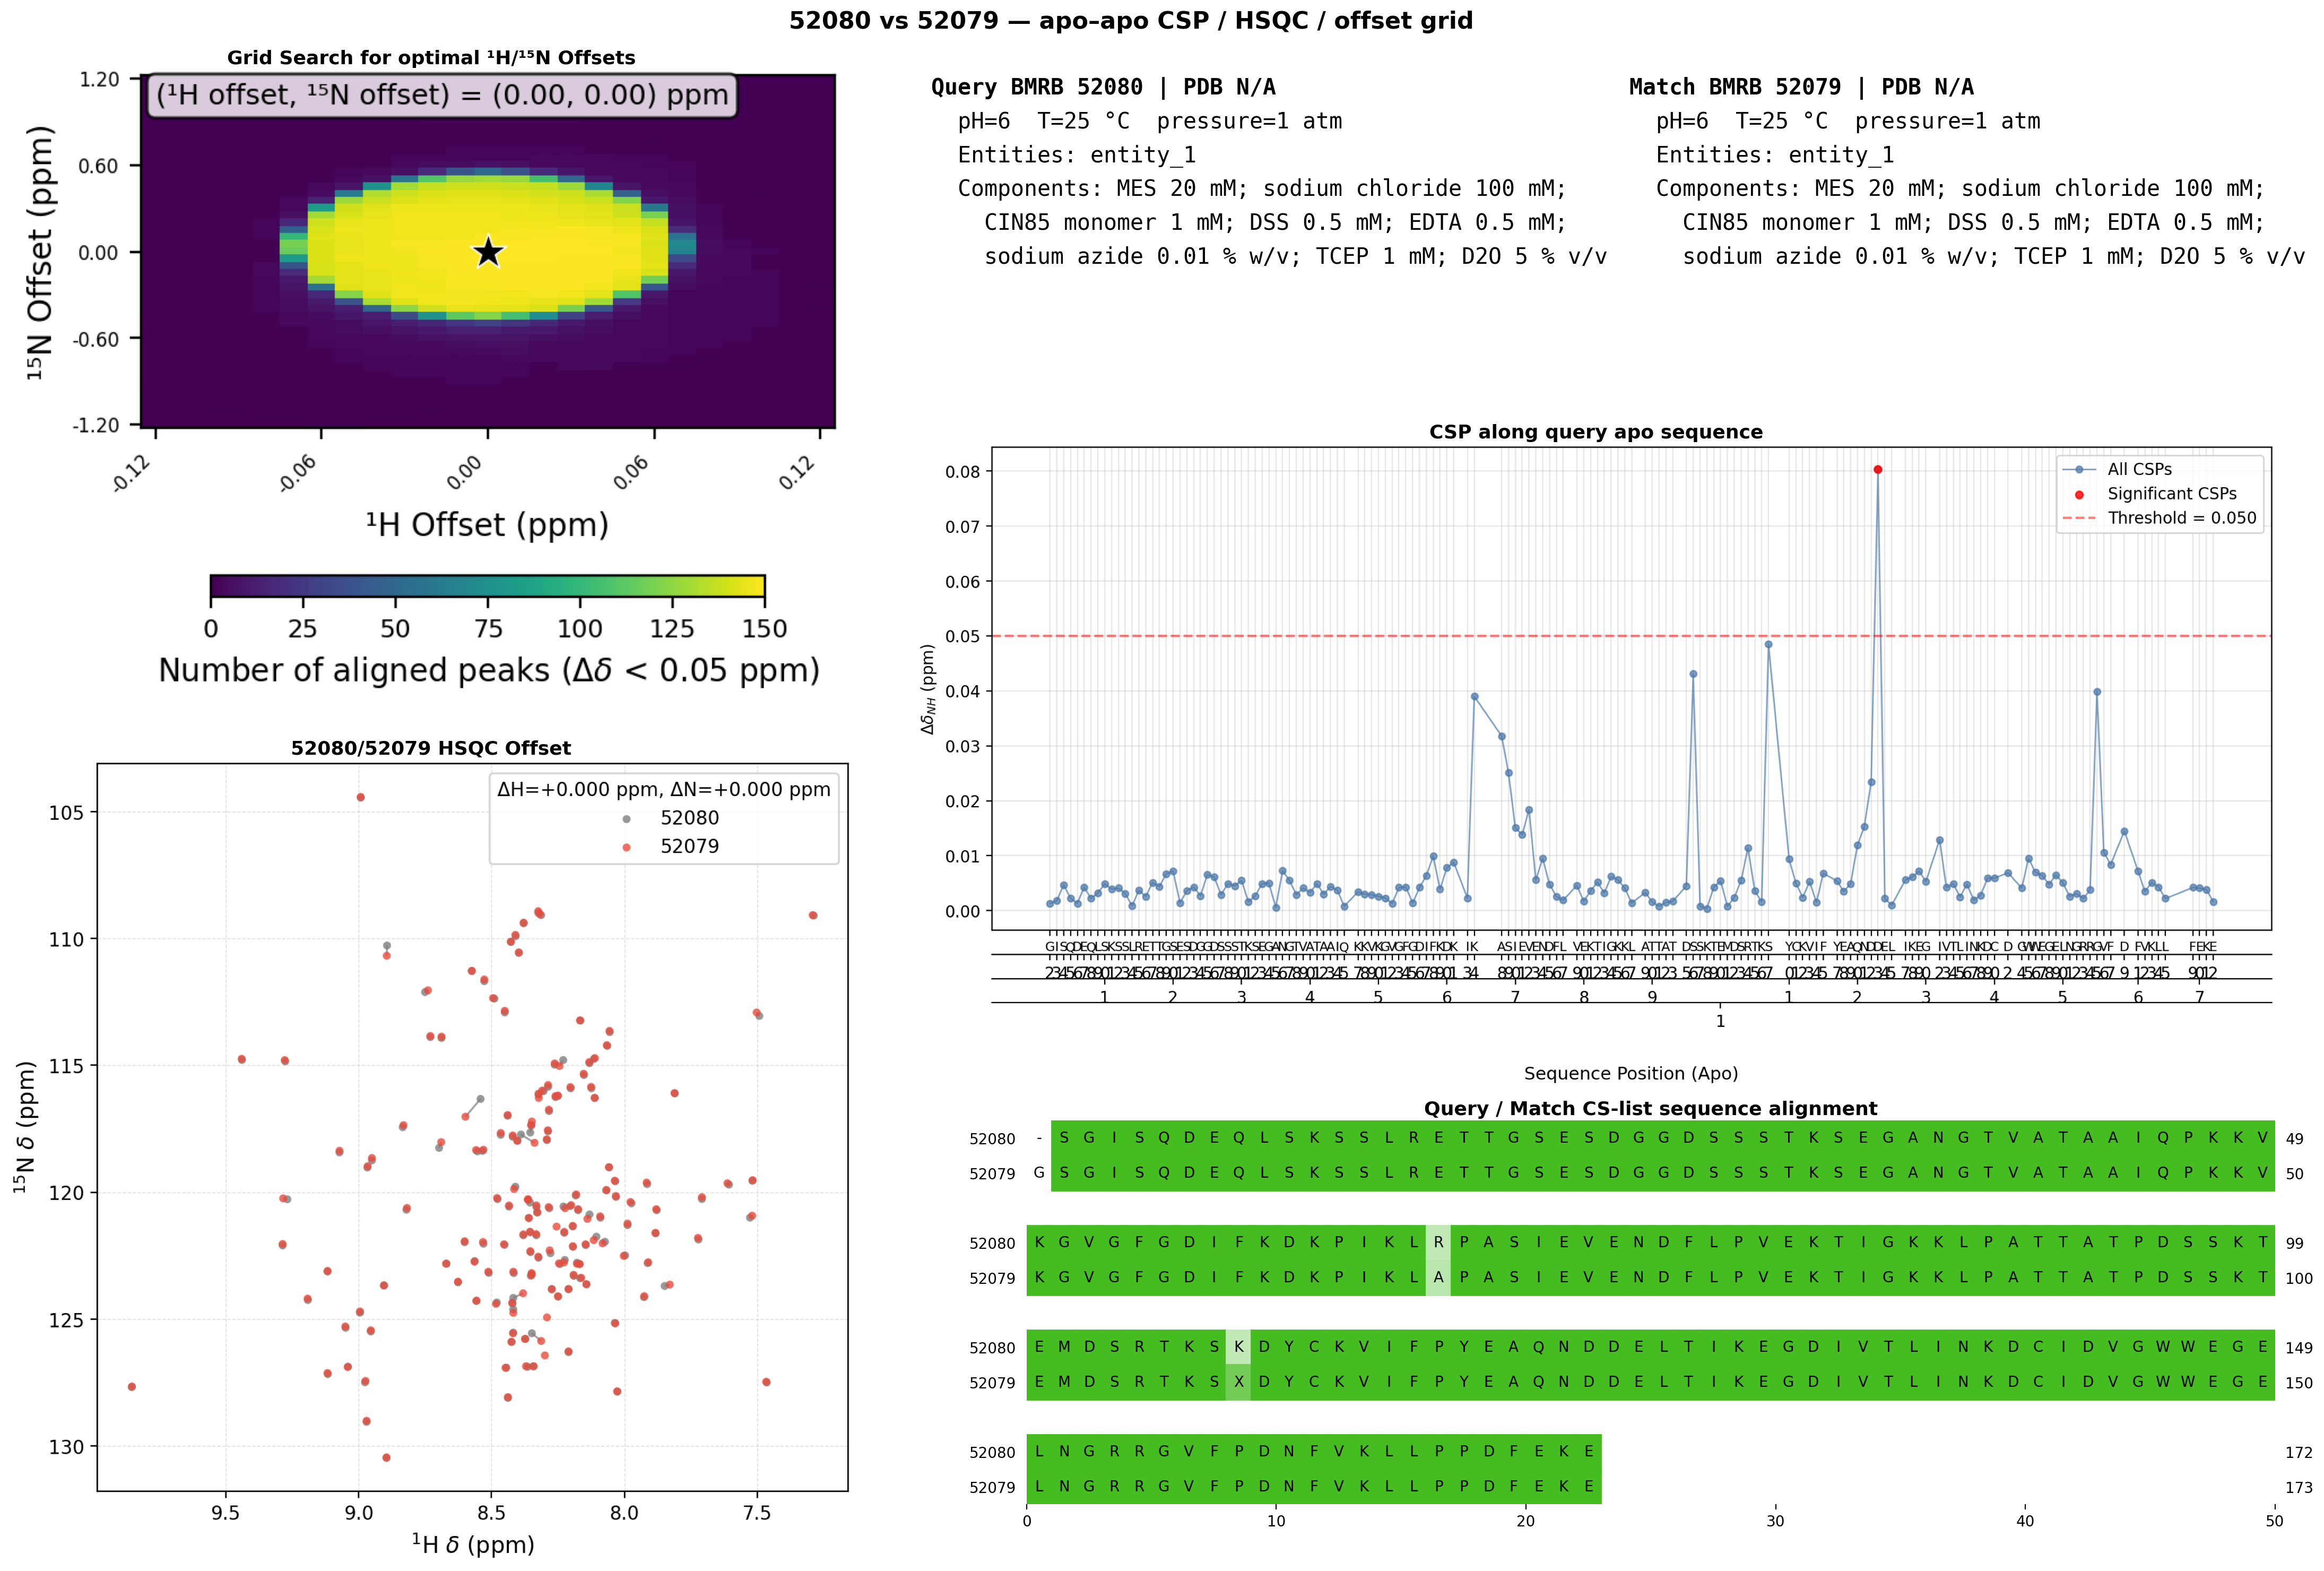
\includegraphics[width=\linewidth]{SF25A_apo_apo_52080_52079.png}
\captionsetup{labelformat=empty}
\caption{\textbf{SI Fig. S25A. Apo vs apo control study for BMRB 52080 and 52079.}
This case involves the CIN85 SH3B--SH3C linker (residues 163--333).
There is a sequence mismatch at R227A (BMRB 52080 is the R229A variant;
BMRB 52079 is R227A/R229A); BMRB 52079 also has an extra N-terminal Gly.
99.3\% of the CSPs for this control are below 0.05\,ppm.}
\end{figure}

\clearpage
\begin{figure}[H]
\centering
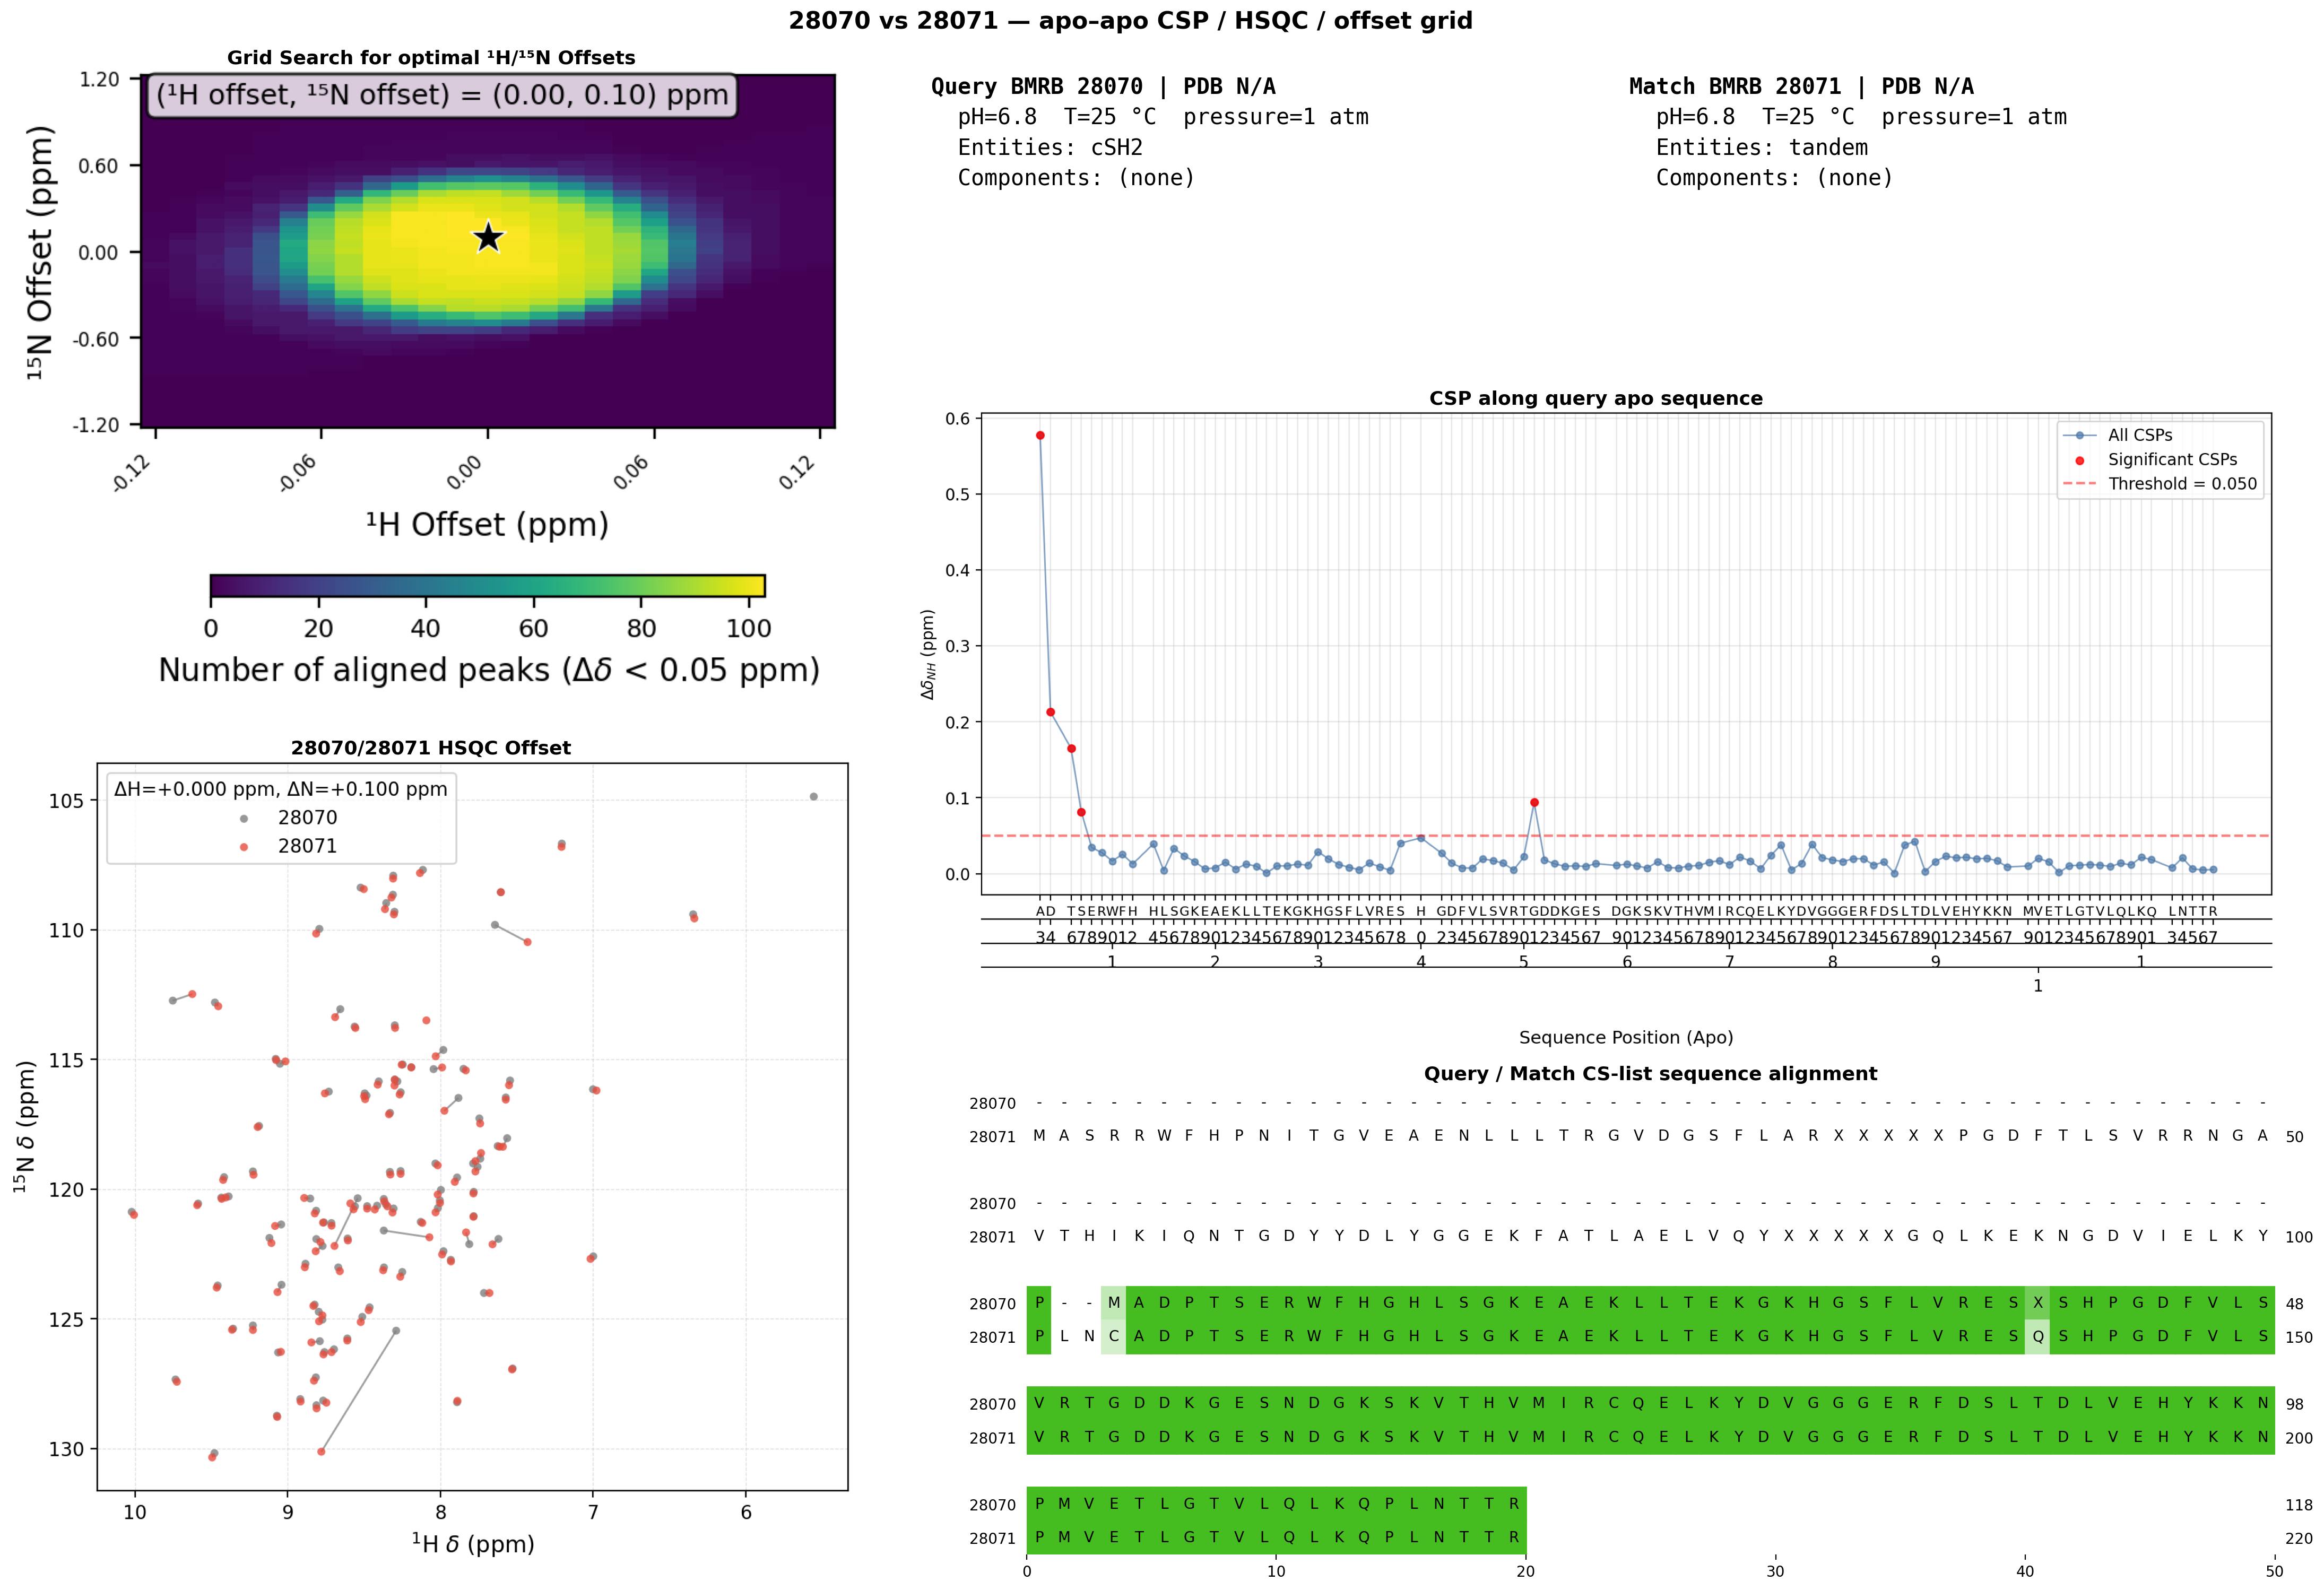
\includegraphics[width=\linewidth]{SF25B_apo_apo_28070_28071.png}
\captionsetup{labelformat=empty}
\caption{\textbf{SI Fig. S25B. Apo vs apo control study for BMRB 28070 and 28071.}
This case involves the SH2 domains of SHP2.
BMRB 28071 is the tandem nSH2--cSH2 construct and includes a large N-terminal
region (the nSH2 domain and inter-SH2 linker, $\sim$100 residues) that is absent
from the isolated cSH2 entry (BMRB 28070).
95.4\% of the CSPs for this control are below 0.05\,ppm.}
\end{figure}

\clearpage
\begin{figure}[H]
\centering
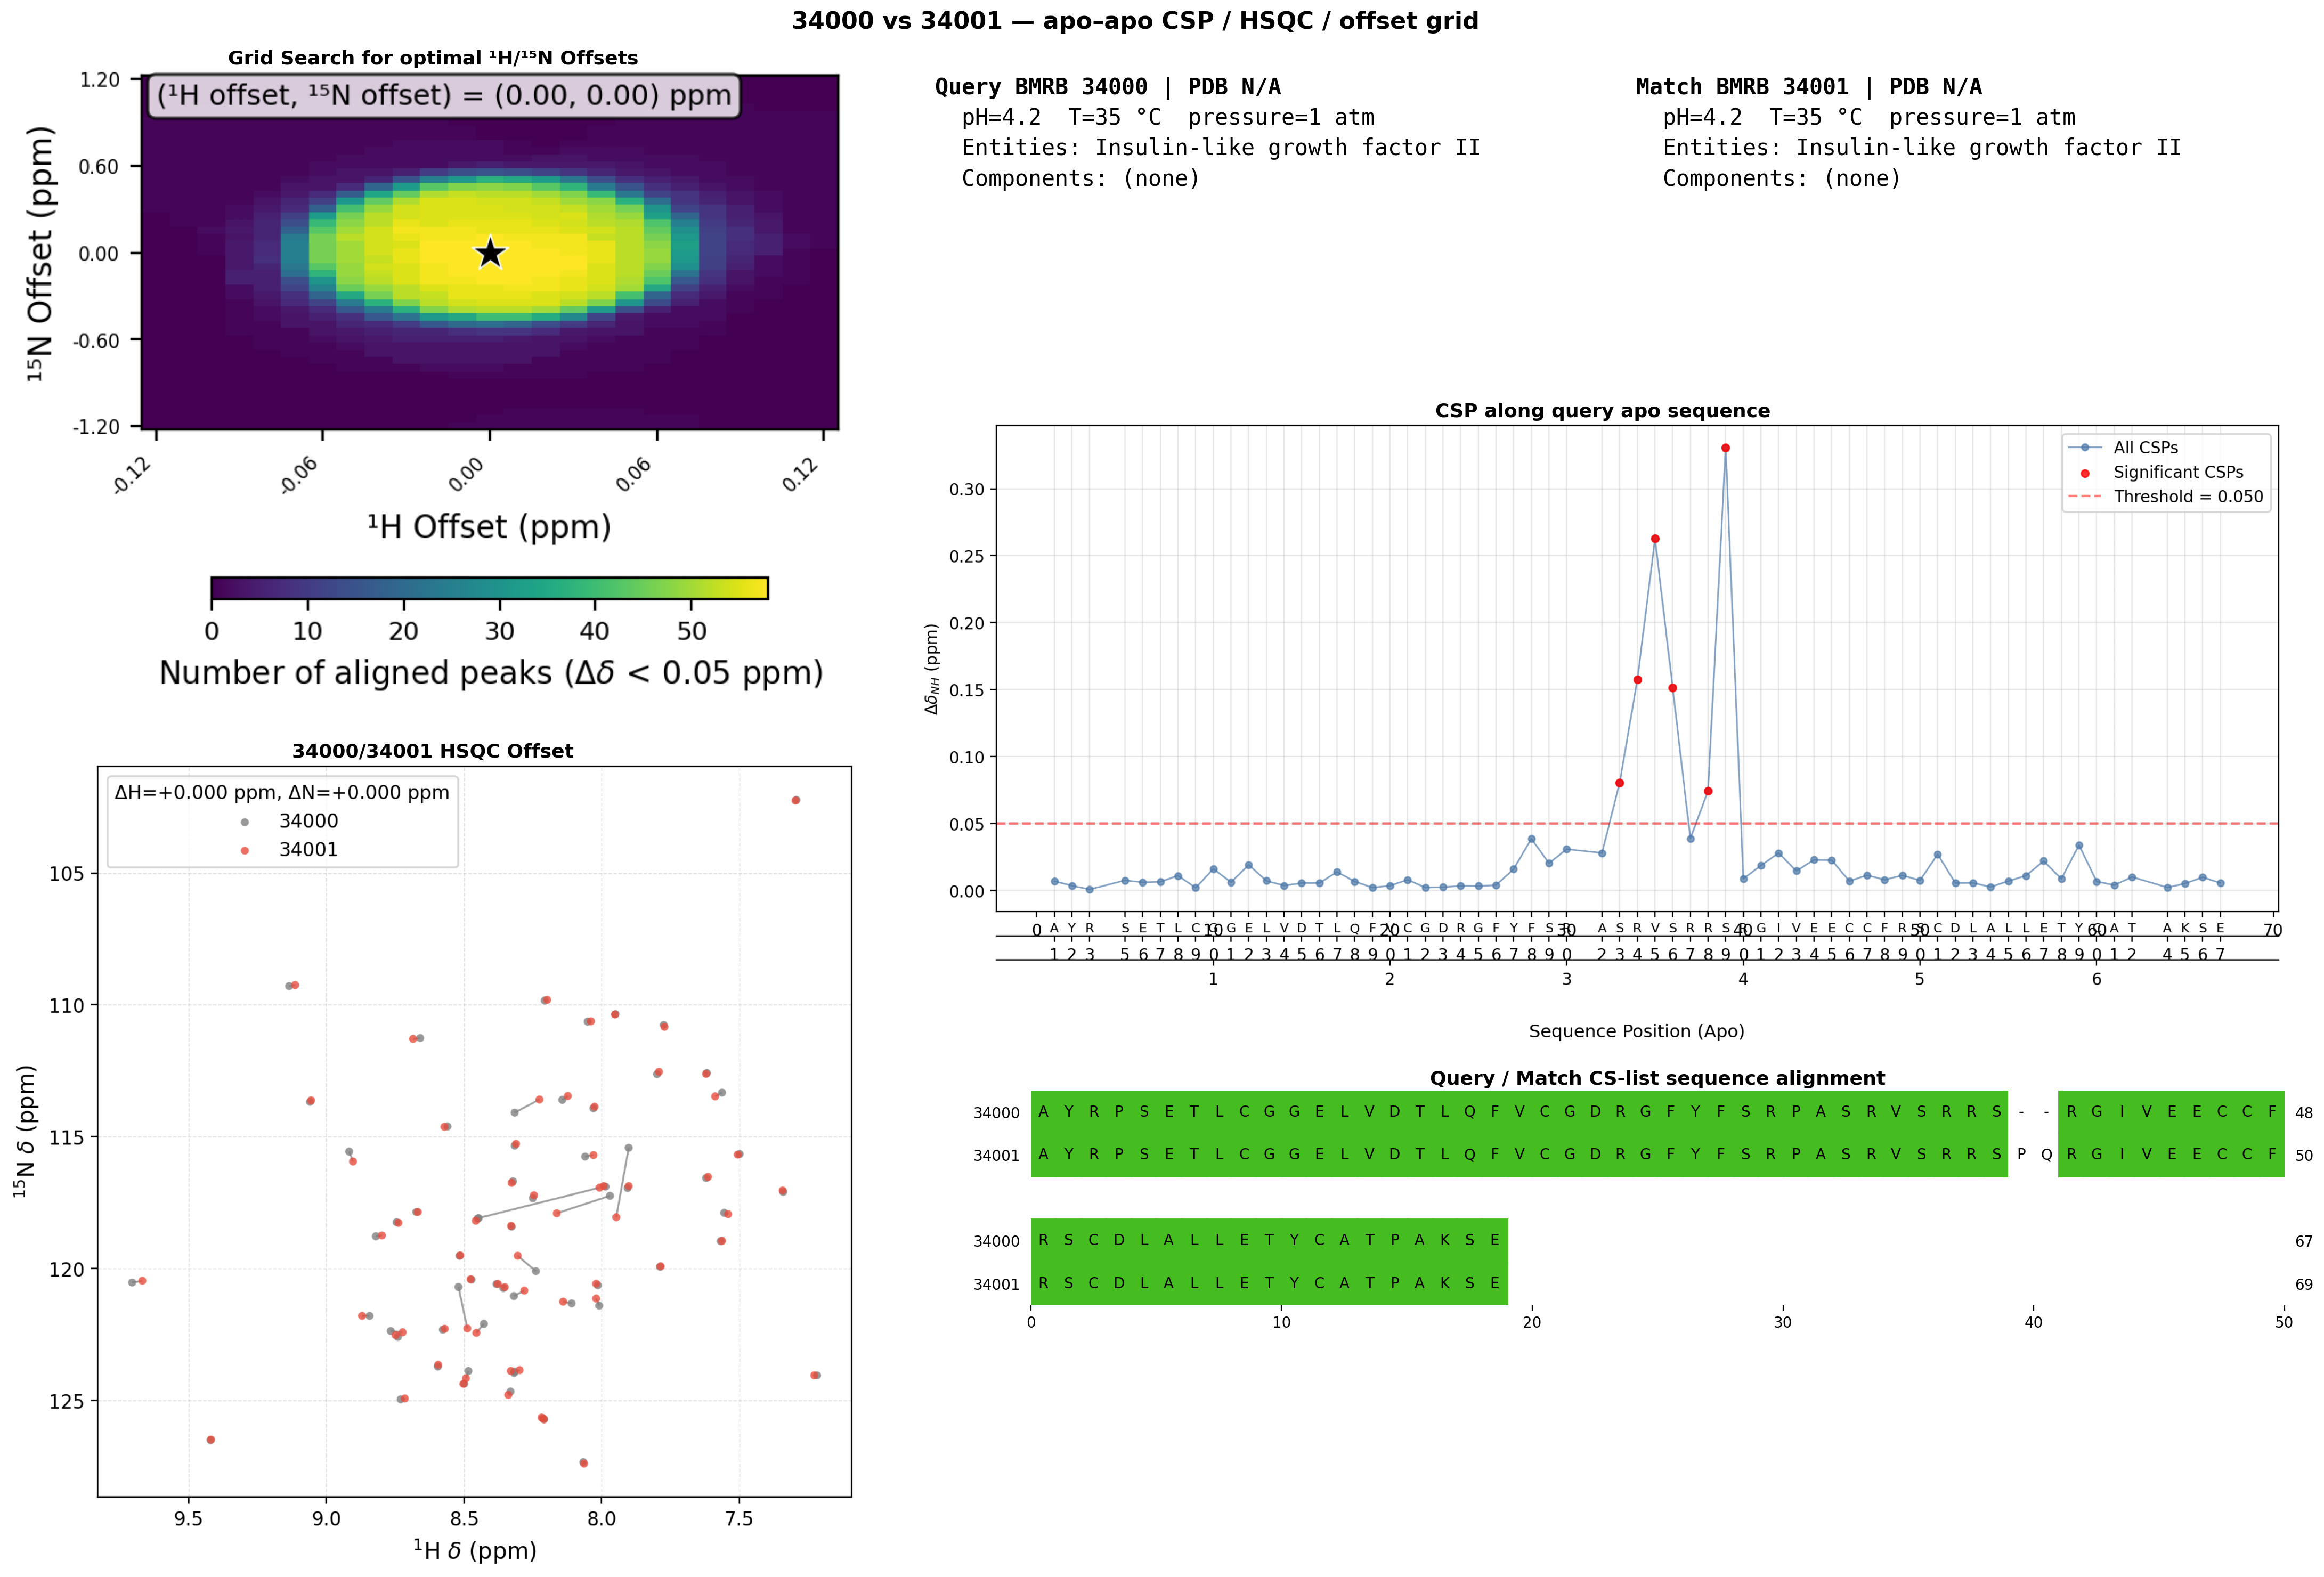
\includegraphics[width=\linewidth]{SF25C_apo_apo_34000_34001.png}
\captionsetup{labelformat=empty}
\caption{\textbf{SI Fig. S25C. Apo vs apo control study for BMRB 34000 and 34001.}
This case involves insulin-like growth factor II (IGF-II).
BMRB 34001 is the [S39\_PQ]-IGF-II variant and contains a two-residue Pro--Gln
insertion after Ser39 relative to wild-type IGF-II (BMRB 34000).
90.6\% of the CSPs for this control are below 0.05\,ppm.}
\end{figure}

\clearpage
\begin{figure}[H]
\centering
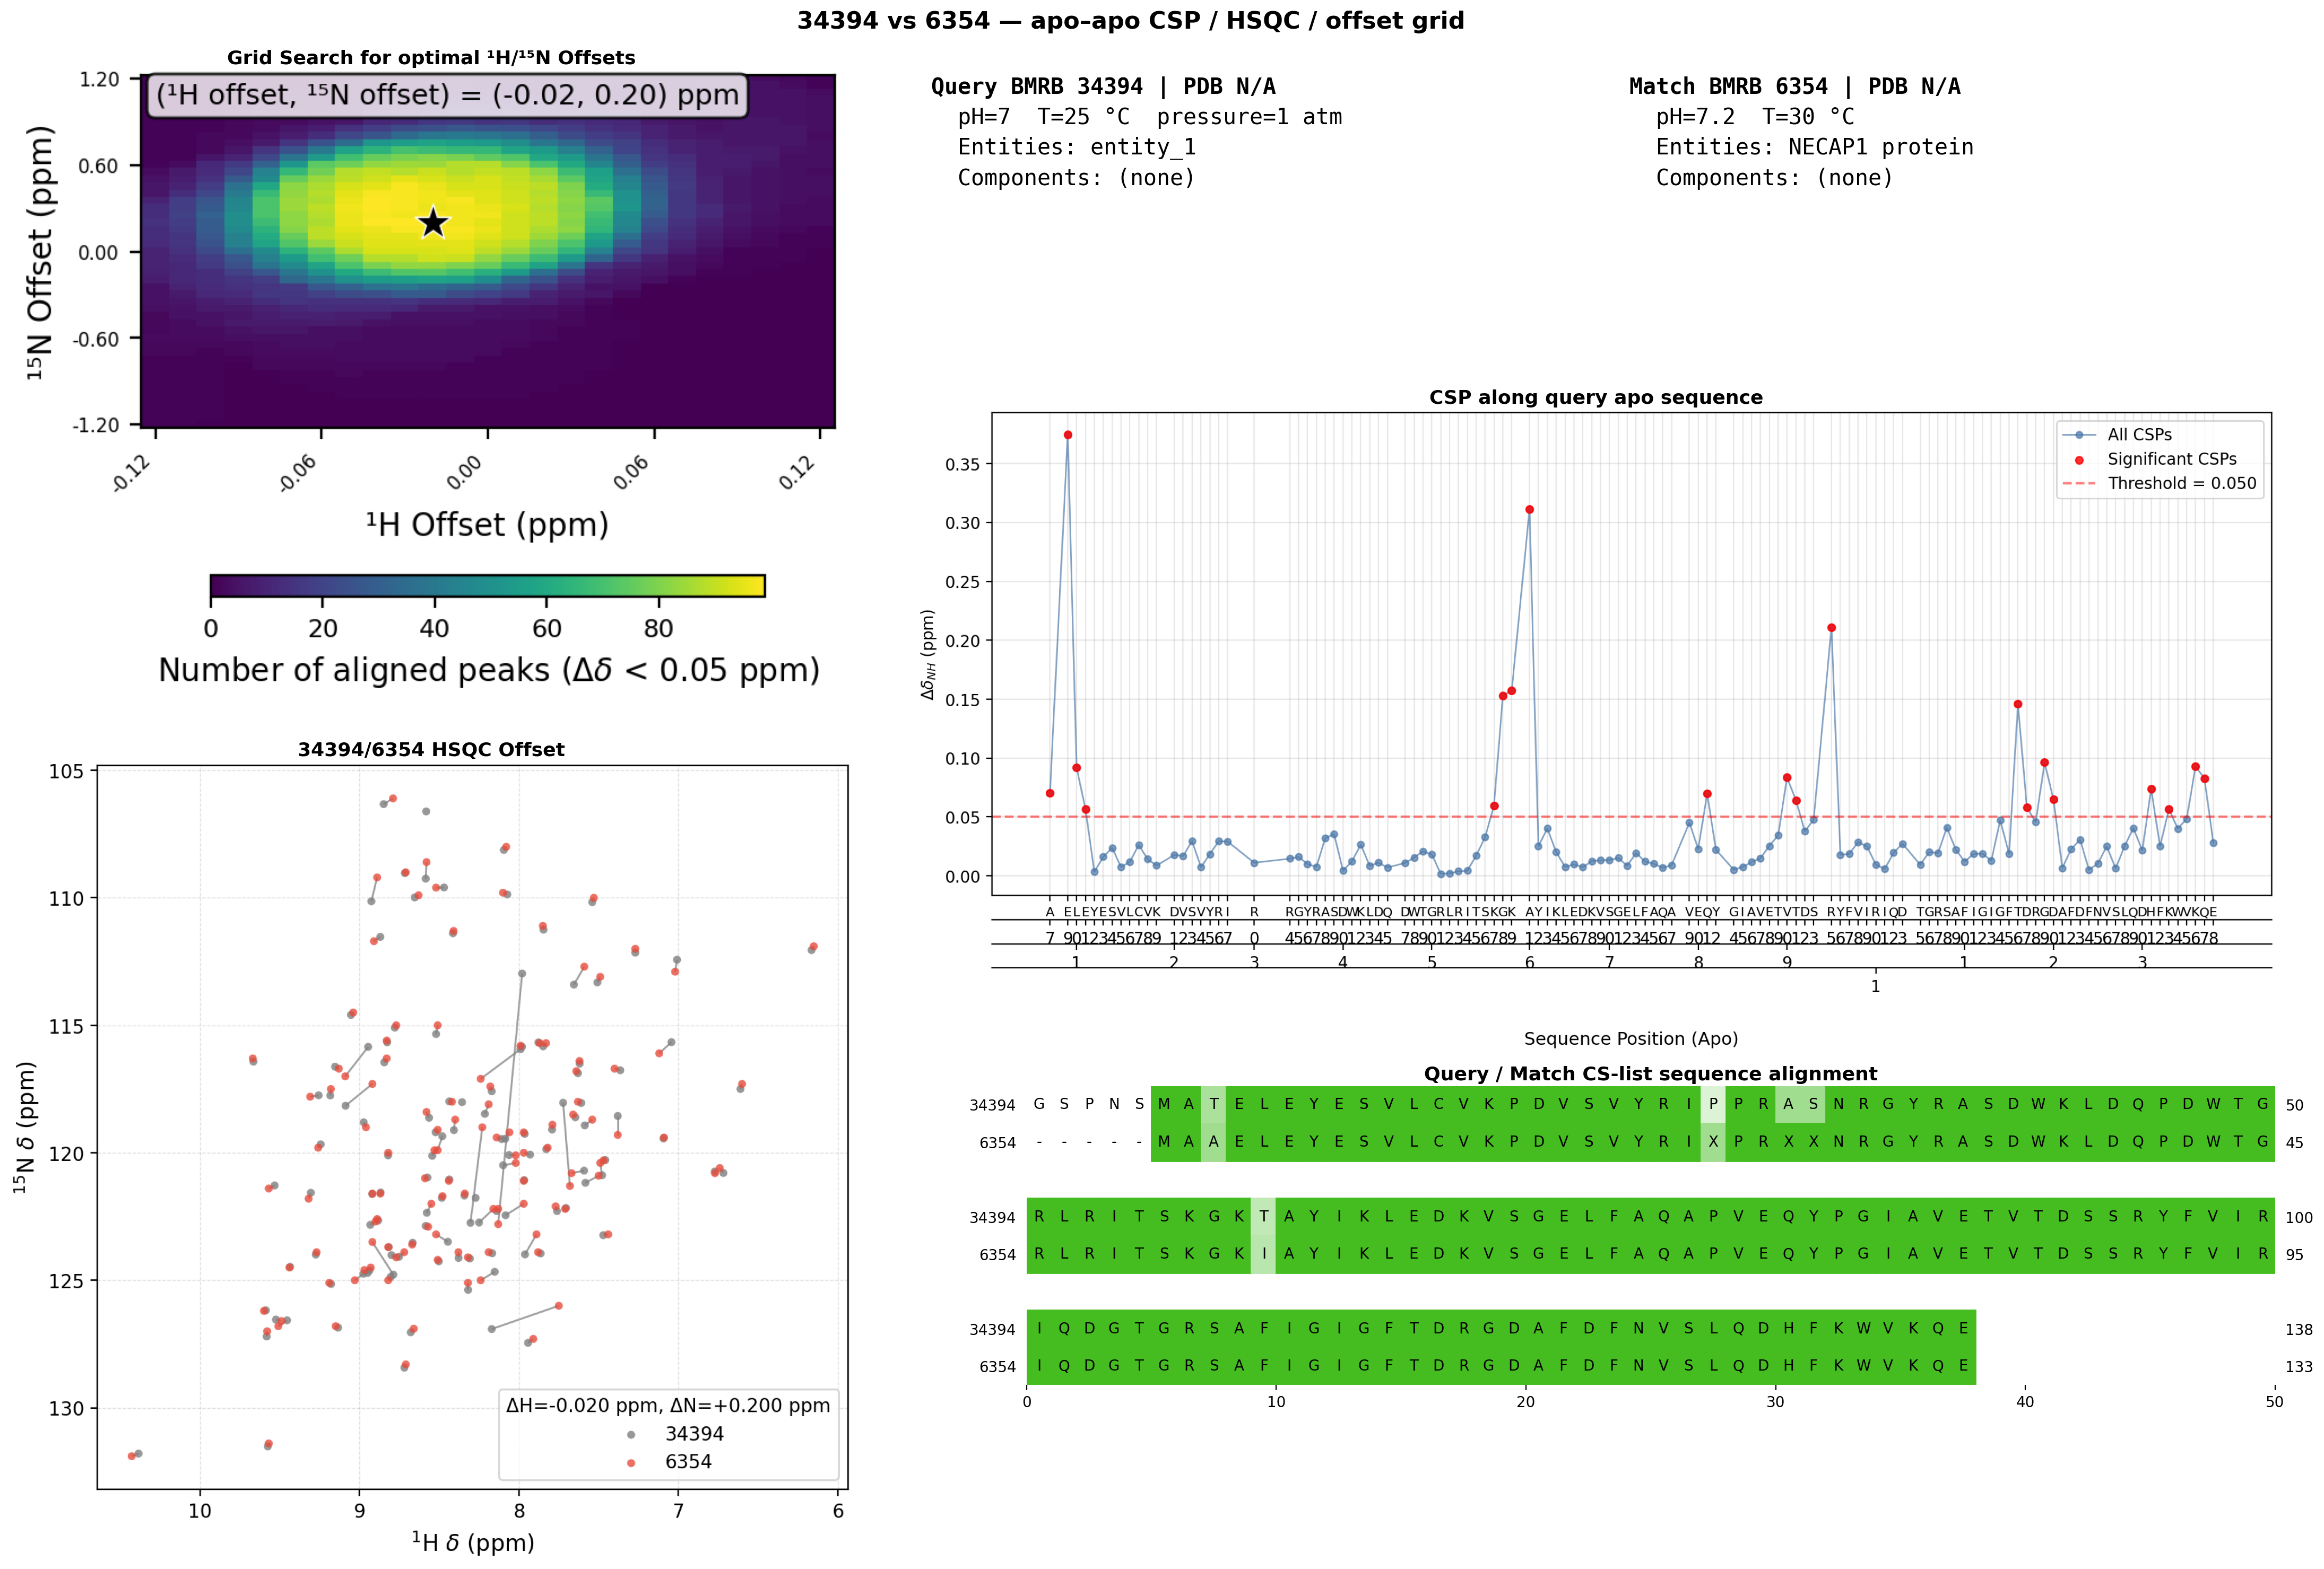
\includegraphics[width=\linewidth]{SF25D_apo_apo_34394_6354.png}
\captionsetup{labelformat=empty}
\caption{\textbf{SI Fig. S25D. Apo vs apo control study for BMRB 34394 and 6354.}
This case involves the NECAP1 PHear domain.
BMRB 34394 has a five-residue N-terminal extension (GSPNS) relative to
BMRB 6354, plus substitutions T8A and K59I and short internal insertions
(Pro28 and Ala31--Ser32) in the 34394 construct.
83.2\% of the CSPs for this control are below 0.05\,ppm.}
\end{figure}

\clearpage
\begin{figure}[H]
\centering
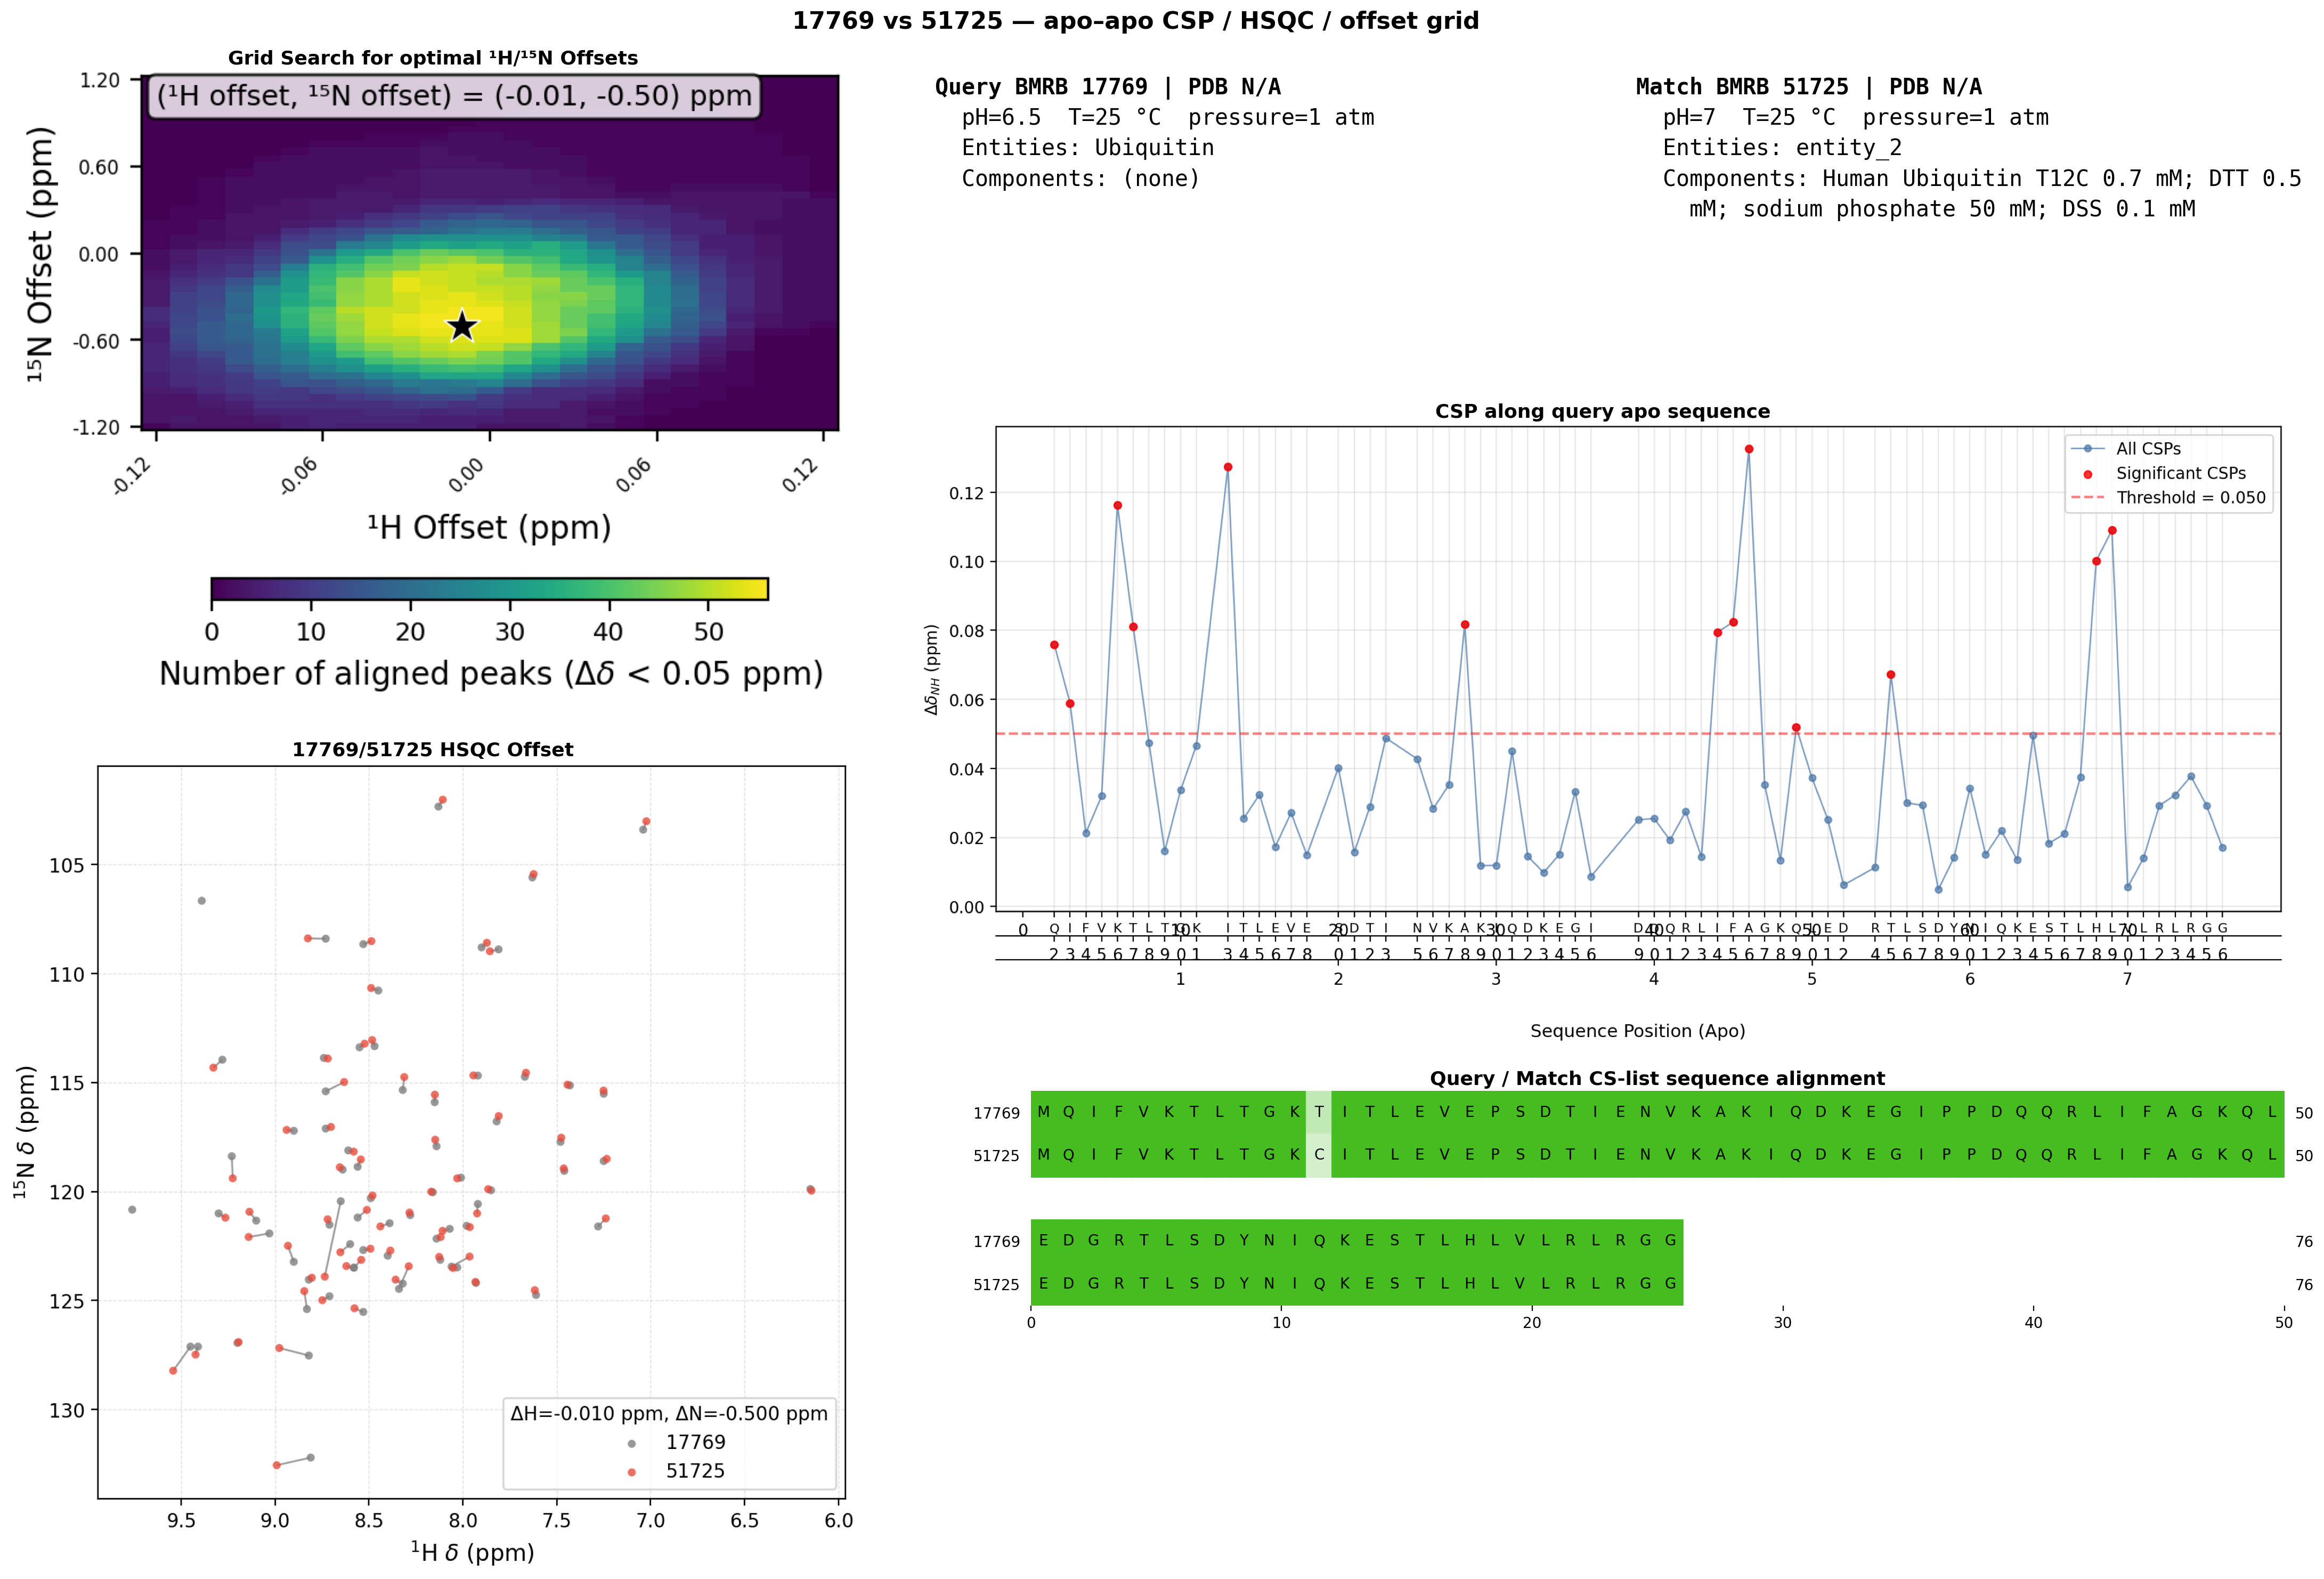
\includegraphics[width=\linewidth]{SF25E_apo_apo_17769_51725.png}
\captionsetup{labelformat=empty}
\caption{\textbf{SI Fig. S25E. Apo vs apo control study for BMRB 17769 and 51725.}
This case involves ubiquitin.
There is a sequence mismatch at position 12 (T12C; wild-type Thr in BMRB 17769,
Cys in BMRB 51725).
81.2\% of the CSPs for this control are below 0.05\,ppm.}
\end{figure}

\clearpage
\begin{figure}[H]
\centering
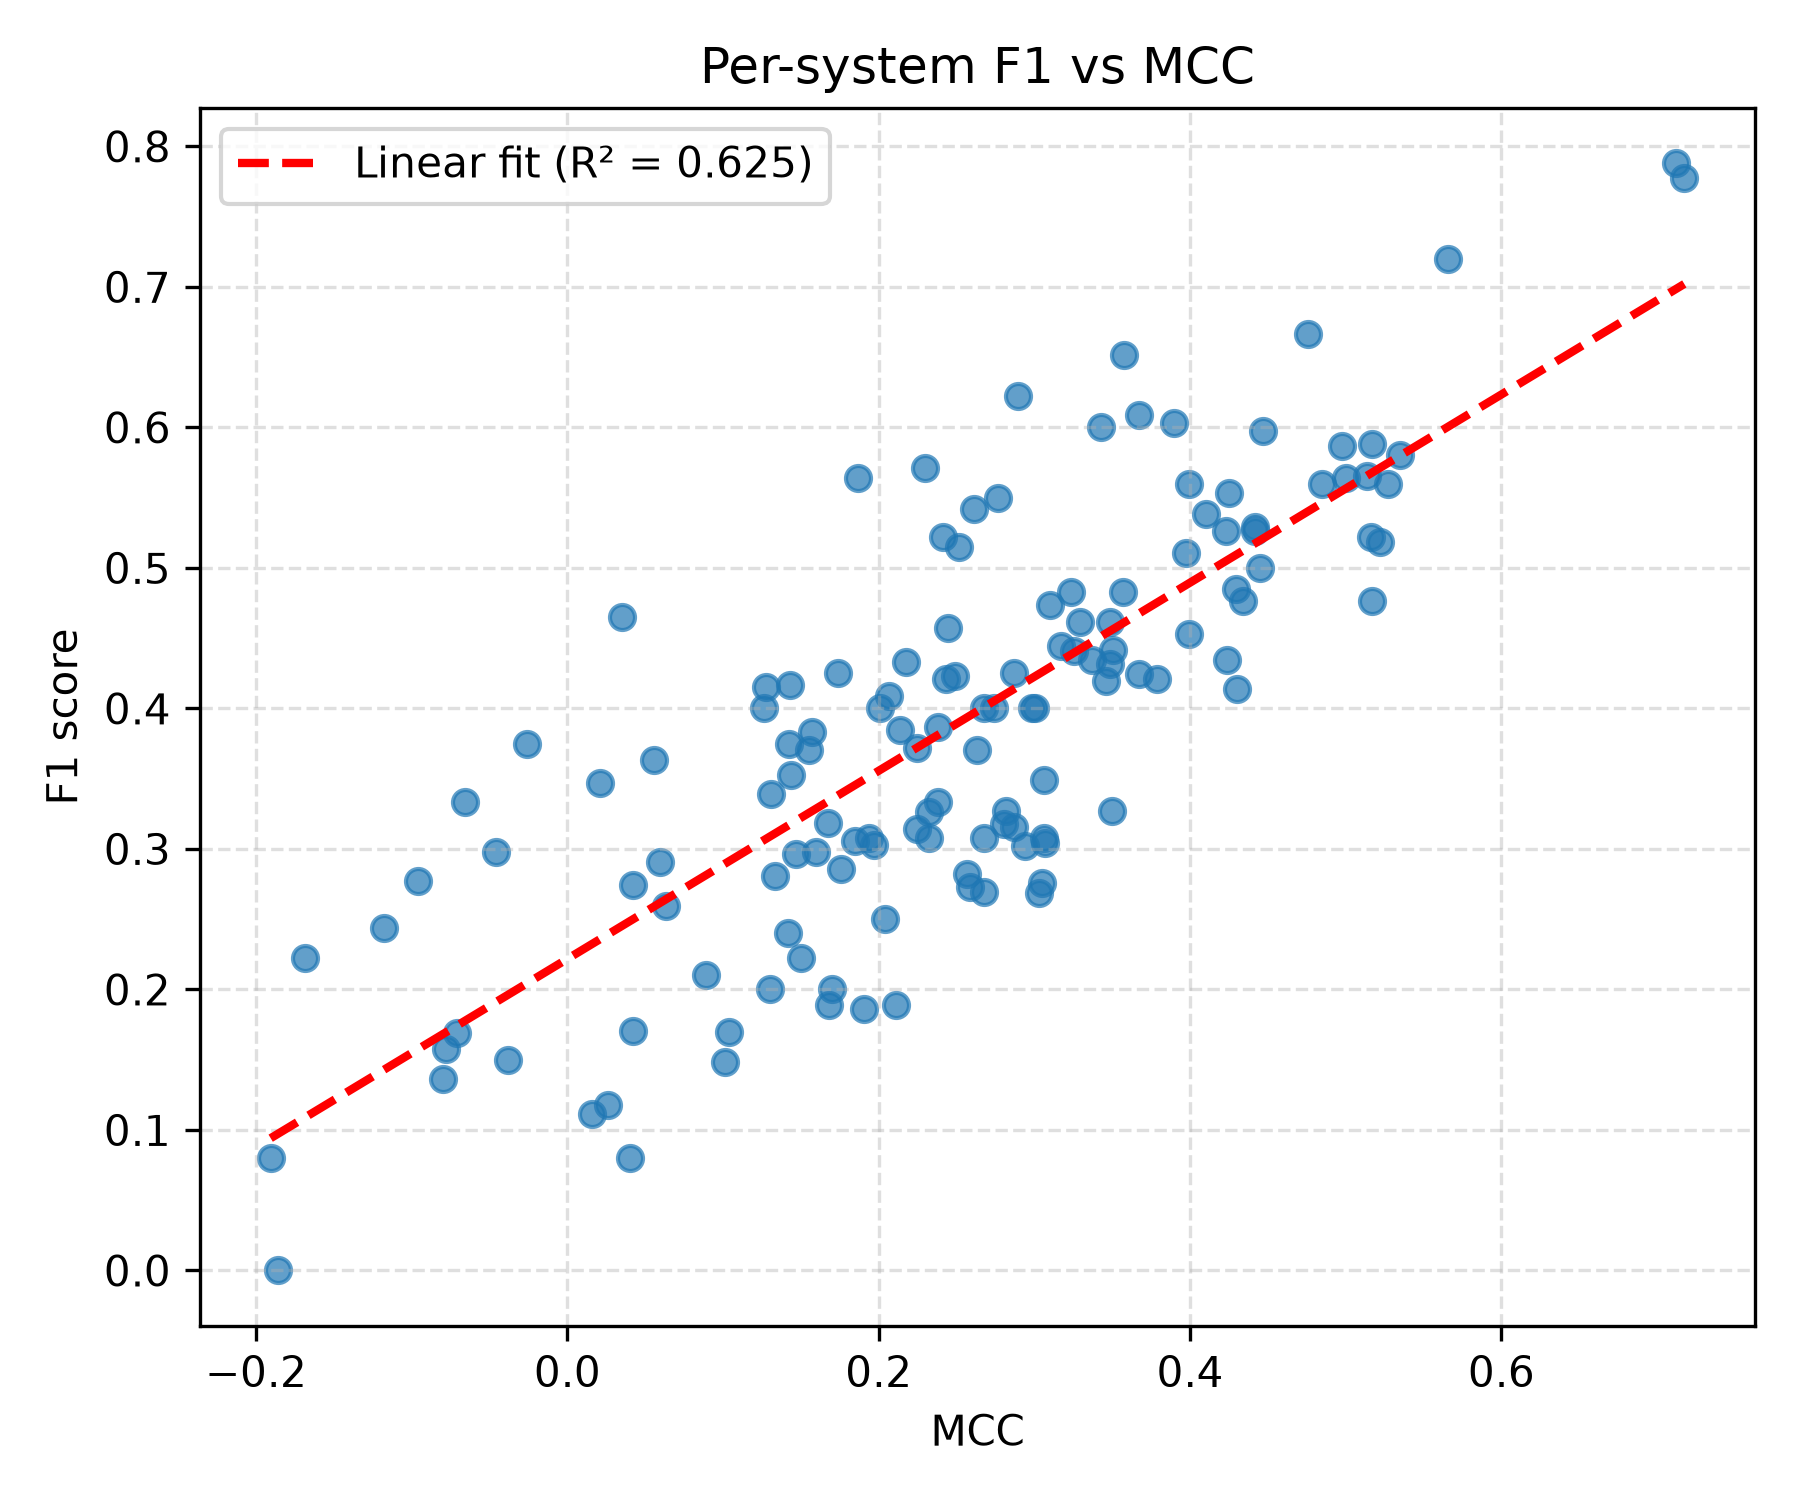
\includegraphics[width=0.9\linewidth]{SF26_f1_vs_mcc.png}
\captionsetup{labelformat=empty}
\caption{\textbf{SI Fig. S26. F1 vs MCC} across the $n=135$ buffer-similar systems
in \texttt{CSP\_UBQ\_ph0.5\_temp5C.csv} with pipeline outputs.}
\end{figure}

\clearpage
\begin{figure}[H]
\centering
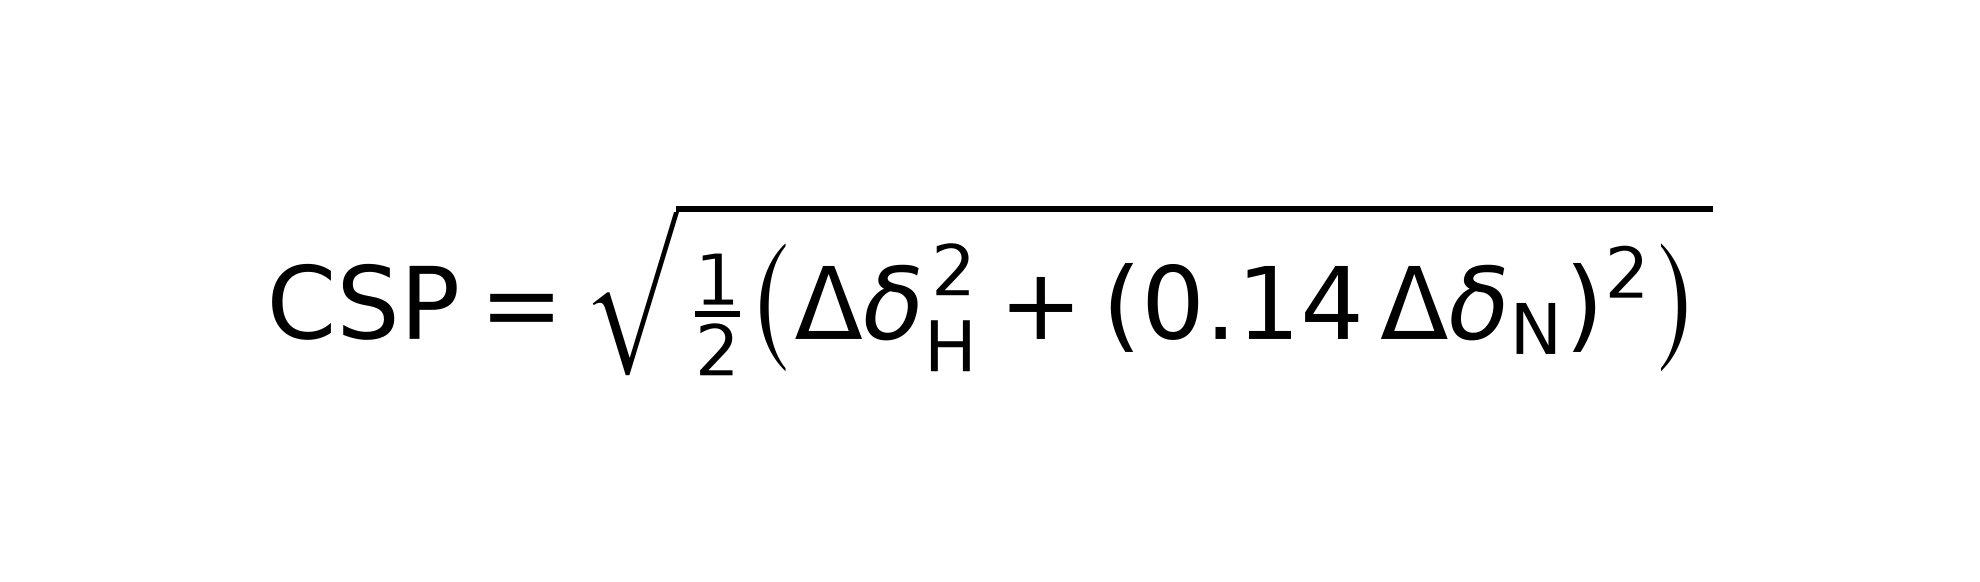
\includegraphics[width=0.7\linewidth]{SE1_nh_csp.png}
\captionsetup{labelformat=empty}
\caption{\textbf{SI Equation S1. Combined HN chemical-shift perturbation}}
\end{figure}

\begin{figure}[H]
\centering
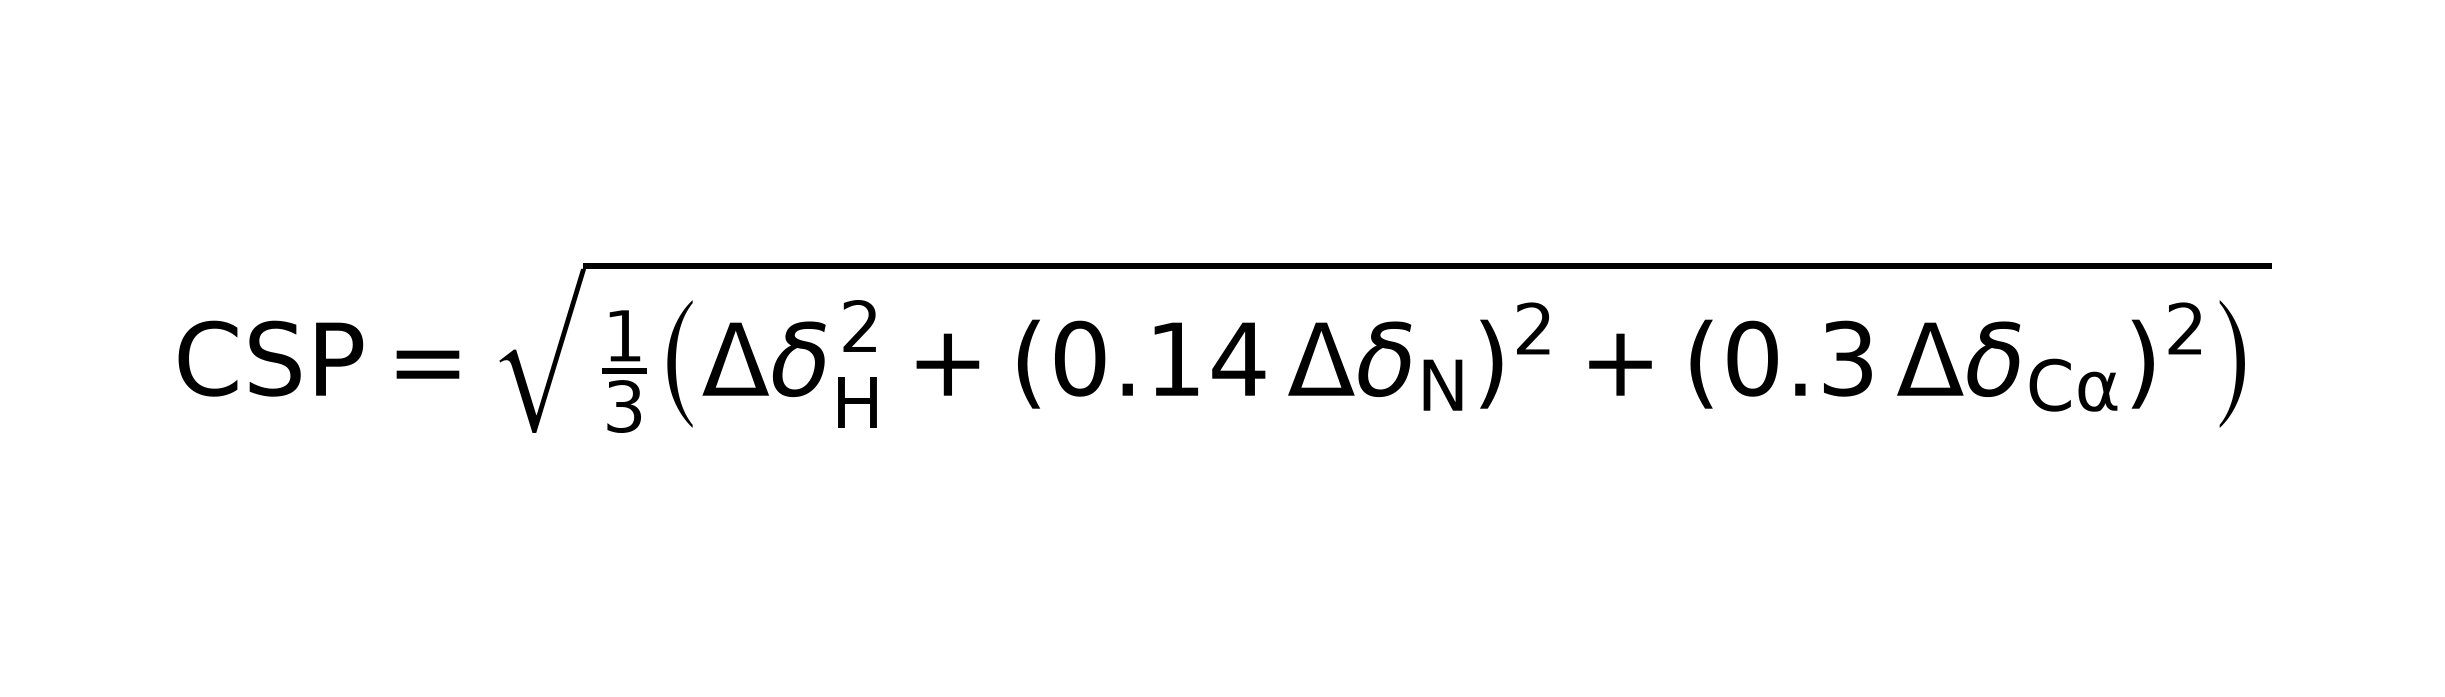
\includegraphics[width=0.7\linewidth]{SE2_nh_ca_csp.png}
\captionsetup{labelformat=empty}
\caption{\textbf{SI Equation S2. Combined HN+C$\alpha$ chemical-shift perturbation}}
\end{figure}

\begin{figure}[H]
\centering
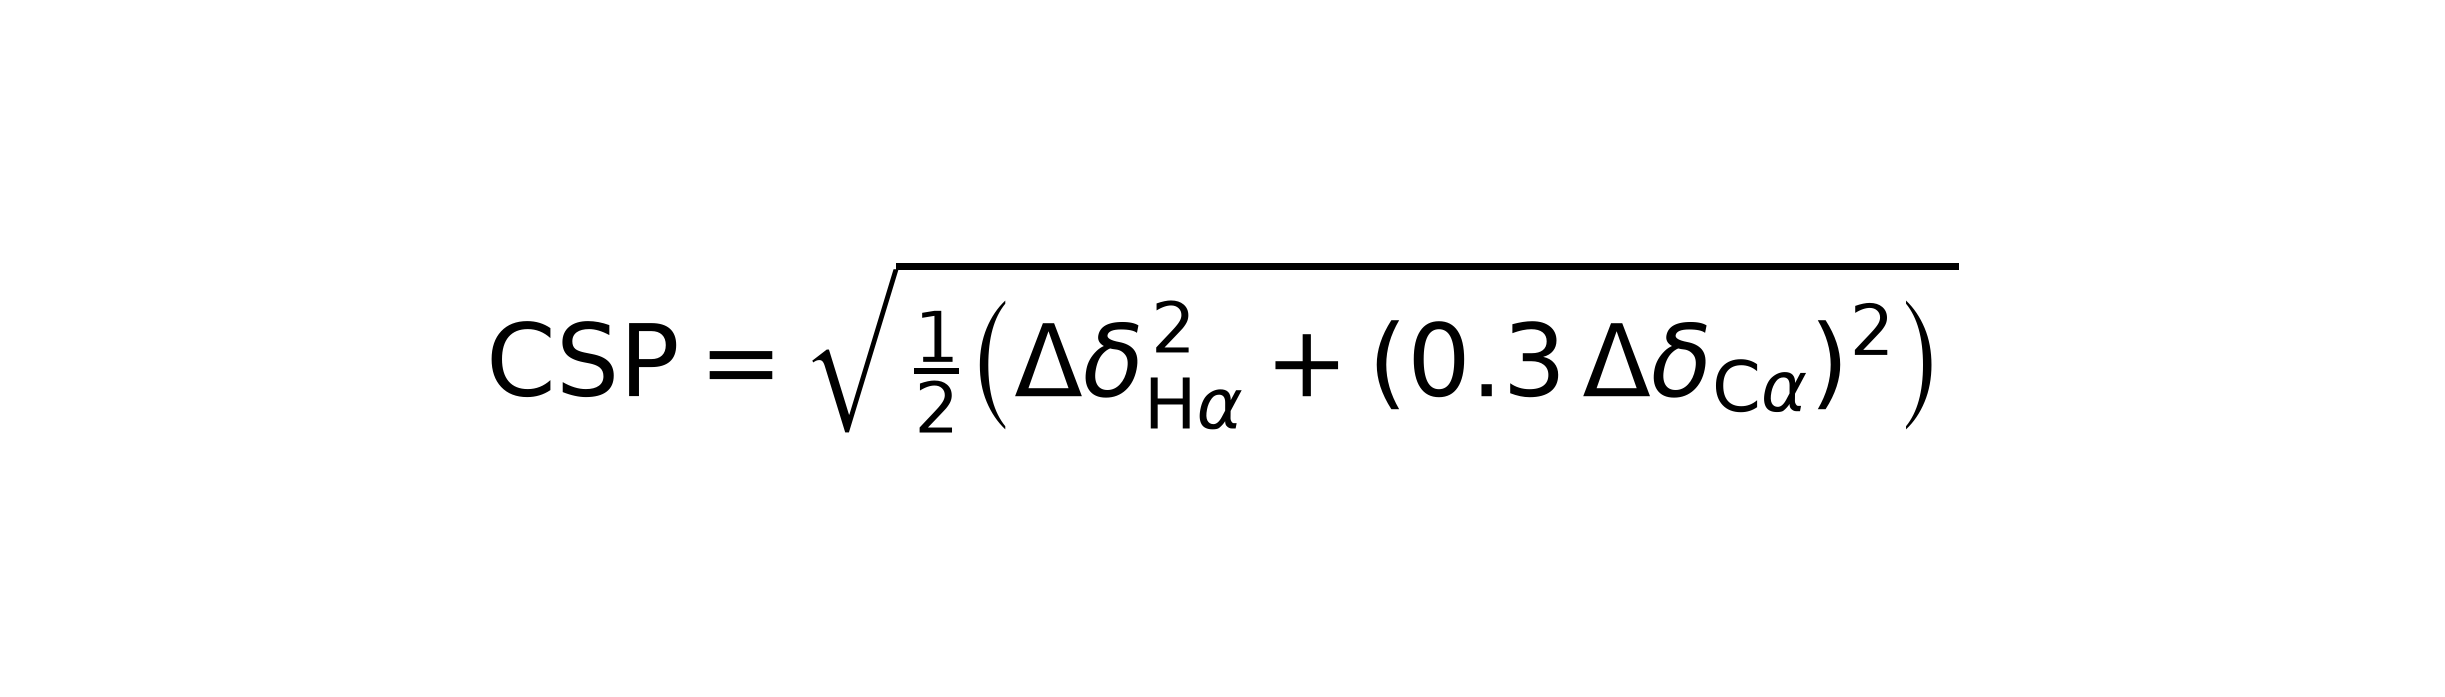
\includegraphics[width=0.7\linewidth]{SE3_ha_ca_csp.png}
\captionsetup{labelformat=empty}
\caption{\textbf{SI Equation S3. Combined H$\alpha$+C$\alpha$ chemical-shift perturbation}}
\end{figure}

\end{document}
